%%%%% Set up %%%%%

% Set document style and font size
\documentclass[12pt]{article}\usepackage[]{graphicx}\usepackage[]{color}
%% maxwidth is the original width if it is less than linewidth
%% otherwise use linewidth (to make sure the graphics do not exceed the margin)
\makeatletter
\def\maxwidth{ %
  \ifdim\Gin@nat@width>\linewidth
    \linewidth
  \else
    \Gin@nat@width
  \fi
}
\makeatother

\definecolor{fgcolor}{rgb}{0.345, 0.345, 0.345}
\newcommand{\hlnum}[1]{\textcolor[rgb]{0.686,0.059,0.569}{#1}}%
\newcommand{\hlstr}[1]{\textcolor[rgb]{0.192,0.494,0.8}{#1}}%
\newcommand{\hlcom}[1]{\textcolor[rgb]{0.678,0.584,0.686}{\textit{#1}}}%
\newcommand{\hlopt}[1]{\textcolor[rgb]{0,0,0}{#1}}%
\newcommand{\hlstd}[1]{\textcolor[rgb]{0.345,0.345,0.345}{#1}}%
\newcommand{\hlkwa}[1]{\textcolor[rgb]{0.161,0.373,0.58}{\textbf{#1}}}%
\newcommand{\hlkwb}[1]{\textcolor[rgb]{0.69,0.353,0.396}{#1}}%
\newcommand{\hlkwc}[1]{\textcolor[rgb]{0.333,0.667,0.333}{#1}}%
\newcommand{\hlkwd}[1]{\textcolor[rgb]{0.737,0.353,0.396}{\textbf{#1}}}%
\let\hlipl\hlkwb

\usepackage{framed}
\makeatletter
\newenvironment{kframe}{%
 \def\at@end@of@kframe{}%
 \ifinner\ifhmode%
  \def\at@end@of@kframe{\end{minipage}}%
  \begin{minipage}{\columnwidth}%
 \fi\fi%
 \def\FrameCommand##1{\hskip\@totalleftmargin \hskip-\fboxsep
 \colorbox{shadecolor}{##1}\hskip-\fboxsep
     % There is no \\@totalrightmargin, so:
     \hskip-\linewidth \hskip-\@totalleftmargin \hskip\columnwidth}%
 \MakeFramed {\advance\hsize-\width
   \@totalleftmargin\z@ \linewidth\hsize
   \@setminipage}}%
 {\par\unskip\endMakeFramed%
 \at@end@of@kframe}
\makeatother

\definecolor{shadecolor}{rgb}{.97, .97, .97}
\definecolor{messagecolor}{rgb}{0, 0, 0}
\definecolor{warningcolor}{rgb}{1, 0, 1}
\definecolor{errorcolor}{rgb}{1, 0, 0}
\newenvironment{knitrout}{}{} % an empty environment to be redefined in TeX

\usepackage{alltt}

% File path to resources (style file etc)
\newcommand{\locRepo}{csas-style}

% Style file for DFO Technical Reports
\usepackage{\locRepo/tech-report}

% header-includes from R markdown entry
\usepackage{float}
\usepackage{makeidx}
\makeindex

%%%%% Variables %%%%%

% New definitions: Title, year, report number, authors
% Protect lower case words (i.e., species names) in \Addlcwords{}, in "TechReport.sty"
\newcommand{\trTitle}{Marine Fish and Invertebrate Atlas: Summarizing Geographic Distribution, Population Indices and Environmental Preferences in the Scotian Shelf and Bay of Fundy (1970-2020)}
\newcommand{\trYear}{2021}
\newcommand{\trReportNum}{nnn}
% Optional
\newcommand{\trAuthFootA}{Email: \href{mailto:Daniel.Ricard@dfo-mpo.gc.ca}{\nolinkurl{Daniel.Ricard@dfo-mpo.gc.ca}} \textbar{} telephone: (506) 851-6216}
\newcommand{\trAuthsLong}{Daniel Ricard \textsuperscript{1} Jamie Emberley \textsuperscript{2} Catalina Gomez \textsuperscript{2} Catriona Regnier-McKellar \textsuperscript{2}}
\newcommand{\trAuthsBack}{Ricard, D., Emberley, J., Gomez, C. and Regnier-McKellar, C.}

% New definition: Address
\newcommand{\trAddy}{\textsuperscript{1}Science Branch\\
Gulf Region\\
Fisheries and Oceans Canada\\
Moncton, New Brunswick, E1C 5K4, Canada\\
\textsuperscript{2}Science Branch\\
Maritimes Region\\
Fisheries and Oceans Canada\\
Dartmouth, Nova Scotia, B2Y 4A2, Canada\\}

% Abstract
\newcommand{\trAbstract}{The summer groundfish research vessel survey on the Scotian Shelf and in the Bay of Fundy started in 1970 and was designed to measure the distribution and abundance of major commercial fish species. Over time, additional information on non-commercial species was collected, and allowed considerable insight into ecosystem function and structure, as documented in many primary publications whose analyses used the survey data. The same groundfish survey database has also been used to produce species status reports, atlases of species distribution and remains an essential source of information for stock assessments in the Maritimes Region of Fisheries and Oceans Canada. This report builds on previous work and former atlases by updating a comprehensive suite of indices to assess population status and environmental preferences of 104 species. For each species, trends in geographic distribution and biomass or abundance were plotted. The spatial extent of distribution was plotted over time to gauge how the area occupied has changed. The relationship between abundance or biomass and spatial extent reflected whether the species distribution expands when abundance or biomass increases. Length frequencies over time depicted any changes in mean size. The plots of condition over time revealed whether individual fish are fatter or thinner than their long term mean. Depth, temperature and salinity preferences were estimated to gauge the range of suitable environmental parameters for each species. Finally, for each stratum, the slope describing how local density varies with regional abundance was estimated.}

% Resume (i.e., French abstract)
\newcommand{\trResume}{Voici le résumé. Lorem ipsum dolor sit amet, consectetur adipisicing elit, sed do eiusmod tempor incididunt ut labore et dolore magna aliqua. Ut enim ad minim veniam, quis nostrud exercitation ullamco laboris nisi ut aliquip ex ea commodo consequat. Duis aute irure dolor in reprehenderit in voluptate velit esse cillum dolore eu fugiat nulla pariatur. Excepteur sint occaecat cupidatat non proident, sunt in culpa qui officia deserunt mollit anim id est laborum.}

\newcommand{\trISBN}{}

\DeclareGraphicsExtensions{.png,.pdf}
%%%%% Start %%%%%

% Start the document
\IfFileExists{upquote.sty}{\usepackage{upquote}}{}

% commands and environments needed by pandoc snippets
% extracted from the output of `pandoc -s`
%% Make R markdown code chunks work
\usepackage{array}
\usepackage{amssymb,amsmath}
\usepackage{color}
\usepackage{fancyvrb}

% From default template:
\newcommand{\VerbBar}{|}
\newcommand{\VERB}{\Verb[commandchars=\\\{\}]}
\DefineVerbatimEnvironment{Highlighting}{Verbatim}{commandchars=\\\{\}}
% Add ',fontsize=\small' for more characters per line
\usepackage{framed}
\definecolor{shadecolor}{RGB}{248,248,248}
\newenvironment{Shaded}{\begin{snugshade}}{\end{snugshade}}
\newcommand{\AlertTok}[1]{\textcolor[rgb]{0.94,0.16,0.16}{#1}}
\newcommand{\AnnotationTok}[1]{\textcolor[rgb]{0.56,0.35,0.01}{\textbf{\textit{#1}}}}
\newcommand{\AttributeTok}[1]{\textcolor[rgb]{0.77,0.63,0.00}{#1}}
\newcommand{\BaseNTok}[1]{\textcolor[rgb]{0.00,0.00,0.81}{#1}}
\newcommand{\BuiltInTok}[1]{#1}
\newcommand{\CharTok}[1]{\textcolor[rgb]{0.31,0.60,0.02}{#1}}
\newcommand{\CommentTok}[1]{\textcolor[rgb]{0.56,0.35,0.01}{\textit{#1}}}
\newcommand{\CommentVarTok}[1]{\textcolor[rgb]{0.56,0.35,0.01}{\textbf{\textit{#1}}}}
\newcommand{\ConstantTok}[1]{\textcolor[rgb]{0.00,0.00,0.00}{#1}}
\newcommand{\ControlFlowTok}[1]{\textcolor[rgb]{0.13,0.29,0.53}{\textbf{#1}}}
\newcommand{\DataTypeTok}[1]{\textcolor[rgb]{0.13,0.29,0.53}{#1}}
\newcommand{\DecValTok}[1]{\textcolor[rgb]{0.00,0.00,0.81}{#1}}
\newcommand{\DocumentationTok}[1]{\textcolor[rgb]{0.56,0.35,0.01}{\textbf{\textit{#1}}}}
\newcommand{\ErrorTok}[1]{\textcolor[rgb]{0.64,0.00,0.00}{\textbf{#1}}}
\newcommand{\ExtensionTok}[1]{#1}
\newcommand{\FloatTok}[1]{\textcolor[rgb]{0.00,0.00,0.81}{#1}}
\newcommand{\FunctionTok}[1]{\textcolor[rgb]{0.00,0.00,0.00}{#1}}
\newcommand{\ImportTok}[1]{#1}
\newcommand{\InformationTok}[1]{\textcolor[rgb]{0.56,0.35,0.01}{\textbf{\textit{#1}}}}
\newcommand{\KeywordTok}[1]{\textcolor[rgb]{0.13,0.29,0.53}{\textbf{#1}}}
\newcommand{\NormalTok}[1]{#1}
\newcommand{\OperatorTok}[1]{\textcolor[rgb]{0.81,0.36,0.00}{\textbf{#1}}}
\newcommand{\OtherTok}[1]{\textcolor[rgb]{0.56,0.35,0.01}{#1}}
\newcommand{\PreprocessorTok}[1]{\textcolor[rgb]{0.56,0.35,0.01}{\textit{#1}}}
\newcommand{\RegionMarkerTok}[1]{#1}
\newcommand{\SpecialCharTok}[1]{\textcolor[rgb]{0.00,0.00,0.00}{#1}}
\newcommand{\SpecialStringTok}[1]{\textcolor[rgb]{0.31,0.60,0.02}{#1}}
\newcommand{\StringTok}[1]{\textcolor[rgb]{0.31,0.60,0.02}{#1}}
\newcommand{\VariableTok}[1]{\textcolor[rgb]{0.00,0.00,0.00}{#1}}
\newcommand{\VerbatimStringTok}[1]{\textcolor[rgb]{0.31,0.60,0.02}{#1}}
\newcommand{\WarningTok}[1]{\textcolor[rgb]{0.56,0.35,0.01}{\textbf{\textit{#1}}}}
\begin{document}

%%%% Front matter %%%%%

% Add the first few pages
\frontmatter

%%%%% Drafts %%%%%

%\linenumbers  % Line numbers
%\onehalfspacing  % Extra space between lines
\renewcommand{\headrulewidth}{0.5pt}  % Header line
\renewcommand{\footrulewidth}{0.5pt}  % footer line
%\pagestyle{fancy}\fancyhead[c]{Draft: Do not cite or circulate}  % Header text

\newcommand{\lt}{\ensuremath <}
\newcommand{\gt}{\ensuremath >}

%Defines cslreferences environment
%Required by pandoc 2.8
%Copied from https://github.com/rstudio/rmarkdown/issues/1649

%%%%% Main document %%%%%
\hypertarget{sec:introduction}{%
\section{Introduction}\label{sec:introduction}}

The summer (July-August) groundfish research vessel survey on the Scotian Shelf and in the Bay of Fundy was started in 1970 by Fisheries and Oceans Canada Maritimes Region. The survey was originally designed to measure the distribution and abundance of major commercial fish species. Over time, information on non-commercial species was also collected. The groundfish survey database storing the information collected during the annual survey provides the main source of fisheries-independent information for marine species in the region. This information is routinely used to support stock assessments, to produce species status reports and has been previously used to publish atlases of species distribution.

The current document is an update of an earlier report (Ricard and Shackell \protect\hyperlink{ref-Ricard:MARatlas:2013}{2013}) that built on former atlases by updating a comprehensive suite of derived indices for 104 species to assess population status and environmental preferences. The information collected during the survey is stored in a relational database management system archived at Fisheries and Oceans Canada Maritimes Region which contains detailed information about the sampling locations and the associated catch. Tow-level survey data is also publicly available from the Ocean Biogeographic Information System (DFO \protect\hyperlink{ref-DFO:2016}{2016}) and (DFO \protect\hyperlink{ref-OpenData_MAR_RV}{2021}). The present atlas follows on the work done by Fisheries and Oceans colleagues from the northern Gulf of St.~Lawrence (Bourdages and Ouellet \protect\hyperlink{ref-Bourdages:NGatlas:2012}{2012}), southern Gulf of St.~Lawrence (Benoît et al. \protect\hyperlink{ref-Benoit:etal:2003:techreport}{2003}) and on earlier work in the Scotian Shelf (Simon and Comeau \protect\hyperlink{ref-Simon:Comeau:1994}{1994}; Horsman and Shackell \protect\hyperlink{ref-Horsman:atlas:2009}{2009}).

To facilitate updates and foster collaboration on the analyses of the survey data, the computer code necessary to extract the data, to perform the analyses presented herein, and to reproduce and update the current document is made available in a git repository (Ricard and Gomez \protect\hyperlink{ref-Ricard-Gomez-2021}{2021}).

The survey area covers three major Northwest Atlantic Fisheries Organization (NAFO) zones that divide the shelf into the colder east 4V and 4W (strata 440-466) and warmer west 4X (strata 470-495). Temporal trends are plotted by NAFO regions for several species. For each species, trends in geographic distribution and biomass or abundance are plotted. Some caution is required in interpreting the results obtained for several taxa due to low sample size as explained later in the text. The spatial extent of distribution is plotted over time to gauge how the area occupied has changed. The relationship between biomass and spatial extent reflects whether the species distribution expands when biomass increases. For each strata, the slope describing how local density varies with regional abundance was estimated (Myers and Stokes \protect\hyperlink{ref-Myers:Stokes:1989}{1989}). These slopes were then plotted against a habitat suitability index to identify important strata for each species. Then, length frequencies over time depicted any changes in mean size. The plots of condition over time revealed whether individual fish are fatter or thinner than their long term mean. Finally, depth, temperature and salinity preferences were estimated to gauge the range of environmental parameters (Perry and Smith \protect\hyperlink{ref-Perry:Smith:1994:cjfas}{1994}). A full ecological interpretation of trends is beyond the scope of this report. Other documents stemming from peer-reviewed scientific processes under the auspices of the \href{https://www.dfo-mpo.gc.ca/csas-sccs/}{Canadian Science Advisory Secretariat} (CSAS) provide further descriptions of spatio-temporal trends in different indicators and put the information collected during the summer groundfish research vessel survey in a more focused context (see for example Clark and Emberley (\protect\hyperlink{ref-ClarkEmberley2011}{2011})).

\hypertarget{methods}{%
\section{Methods}\label{methods}}

\hypertarget{survey-description}{%
\subsection{Survey Description}\label{survey-description}}

The survey is conducted annually in July-August and covers the Scotian Shelf and the Bay of Fundy (Figure~\ref{fig:map1}). It normally involves two separate two-week trips on board an offshore fisheries vessel from the Canadian Coast Guard.

A number of changes in fishing gear type and vessels used occurred since the onset of sampling activities (Clark and Emberley \protect\hyperlink{ref-ClarkEmberley2011}{2011}).


\begin{figure}[htb]

{\centering \pdftooltip{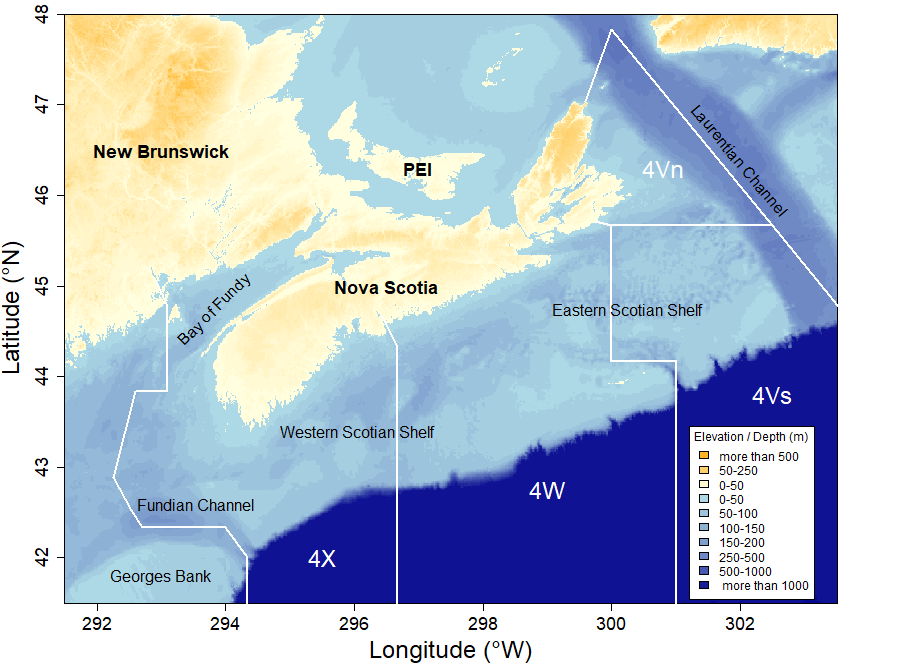
\includegraphics[width=6in]{./figures/annotated-map-NAFO}}{Figure \ref{fig:map1}} 

}

\caption{Map of the Scotian Shelf and Bay of Fundy.}\label{fig:map1}
\end{figure}
\hypertarget{sampling-design}{%
\subsection{Sampling Design}\label{sampling-design}}

The summer survey covers divisions 4V, 4W and 4X of the Northwest Atlantic Fisheries Organization (NAFO) which includes the Scotian Shelf and the Bay of Fundy. The eastern limit of the survey is the Laurentian Channel and the western limit is the Fundian Channel (Figure~\ref{fig:map1}).

The survey follows a stratified random design (Doubleday and Rivard \protect\hyperlink{ref-DoubledayRivard1981}{1981}; Lohr \protect\hyperlink{ref-Lohr1999}{1999}) (Figure~\ref{fig:map2}). The number of tows conducted in each stratum is approximately proportional to its surface area.


\begin{figure}[htb]

{\centering \pdftooltip{
\includegraphics[width=6in]{./figures/SUMMER-strata-map}}{Figure \ref{fig:map2}} 

}

\caption{Map of the Summer survey strata.}\label{fig:map2}
\end{figure}
The basic sampling unit of the survey is a 30-minute fishing tow conducted at a speed of 3.5 knots. This yields a distance towed of 1.75 nautical miles.

After each tow the catch is sorted by species and weighed. Each fish caught is then measured, and further sampling of individual fish weight, maturity status and age are performed for different length classes. When catches exceed 300 individuals, a random sub-sample is used to obtain the length and weight measurements.

The location of representative tows appears in Figure~\ref{fig:map3}.


\begin{figure}[htb]

{\centering \pdftooltip{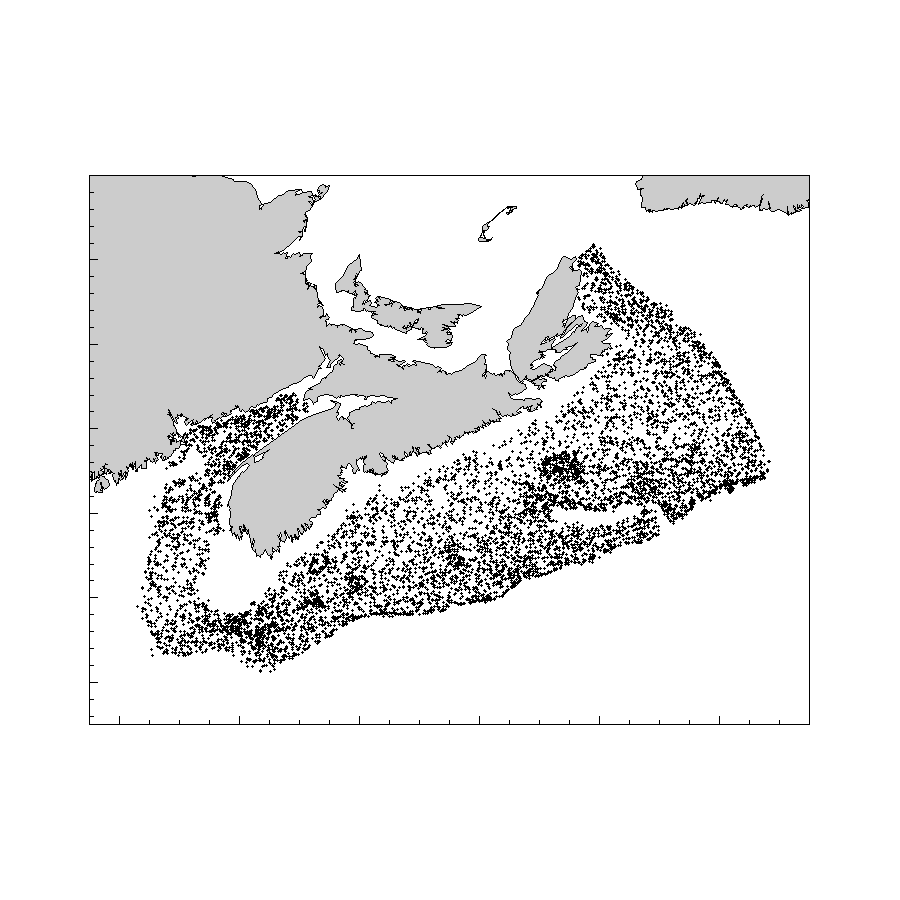
\includegraphics[width=6in]{./figures/SUMMER-tows-map}}{Figure \ref{fig:map3}} 

}

\caption{Map of the Summer survey tows.}\label{fig:map3}
\end{figure}
\hypertarget{taxo}{%
\subsection{Taxonomic Levels}\label{taxo}}

Fish species caught during the surveys are identified by trained scientific personnel and their scientific name is determined. An internal species code used in the relational database is reported for each species (Losier and Waite \protect\hyperlink{ref-LosierWaite1989}{1989}).

By its nature as a bottom trawl, the fishing gear used in the survey catches certain species better than others. To ensure that meaningful ecological information can be extracted from catch samples, we report the catch records for the subset of species that are caught reliably by the gear. To appear in this atlas, a species must have had a minimum of 10 observations over the duration of the survey activities. While both catch abundance and weight are recorded, the weight of species that appear at low abundances is often recorded as zero in the earlier parts of the survey when scales of appropriate precision were not available.

We divided the species caught into five categories based on 1) their taxonomic classification, 2) the number of recorded observations, and 3) their period of valid identification (Table~\ref{tab:taxocat}). Category ''LF'', for ''long frequent'', was assigned to species that have more than 1000 records since 1970 and have been consistently identified since the onset of the survey. Category ''LI'', for ''long intermediate'', was assigned to species that had between 1000 and 200 catch records. Rare and elusive species (those with less than 200 catch records over the duration of the survey) are also reported but to a lower level of analytical details (Category ''LR'', for ''long rare''). Category ''SF'', for ''short frequent'', was assigned to invertebrate species that were consistently sampled only since 1999 (Tremblay M. J. \protect\hyperlink{ref-Tremblayetal:2007}{2007}). And category ''SR'', for ''short rare'' for invertebrate species consistently sampled only since 1999 and with less than 200 catch records.
\begin{table}
\begin{tabular}{p{0.1\textwidth}p{0.2\textwidth}p{0.7\textwidth}}
\toprule
\bfseries{Category} & \bfseries{Name} & \bfseries{Description} \\
\midrule
L & \multicolumn{2}{l}{long - consistently identified since the onset of the survey in 1970}\\
\midrule
LF & long frequent & species that have more than 1000 catch records \\

LI & long intermediate & species that had between 1000 and 200 catch records\\

LR & long rare & species with less than 200 catch records\\
\midrule
S & \multicolumn{2}{l}{short - invertebrate species that were consistently sampled only since 1999}\\
\midrule
SF & short frequent & species with more than 200 catch records \\

SR & short rare & species with less than 200 catch records\\
\bottomrule
\end{tabular}
\caption{Taxonomic levels}
\label{tab:taxocat}
\end{table}
The list of taxa covered in this document is presented in phylogenetic order (Nelson J. S. et al. \protect\hyperlink{ref-Nelsonetal:2004}{2004}) in Table~\ref{tab:tabspecies}. To ensure concordance with authoritative taxonomic information, the AphiaID from the World Register of Marine Species is also provided in Table~\ref{tab:tabspecies} (Appeltans et al. \protect\hyperlink{ref-WoRMS}{2012}).


\begin{landscapepage}
\begingroup\fontsize{9}{11}\selectfont
\begin{longtable}[t]{ccc>{\centering\arraybackslash}p{3cm}>{\centering\arraybackslash}p{3cm}>{\centering\arraybackslash}p{3cm}>{}c>{}ccc}
\caption{\label{tab:tabspecies}List of species included in the Atlas. The species reported here are listed in phylogenetic order as per Page L. M. et al. (\protect\hyperlink{ref-page:etal:7thedition}{2013}). For each taxonomic order and class, each species is listed in the table, its taxonomic family and scientific name is provided, along with its French and English common names, the species code used in the survey database, its AphiaID and a link to the World Registry of Marine Species, its number of catch records in the survey database and its classification category as defined in section~\ref{taxo}.}\\
\toprule
 &  & Family & Scientific name & English name & French name & Species code & AphiaID & Num. records & Category\\
\midrule
\endfirsthead
\caption*{}\\
\toprule
 &  & Family & Scientific name & English name & French name & Species code & AphiaID & Num. records & Category\\
\midrule
\endhead

\endfoot
\bottomrule
\endlastfoot
\addlinespace[0.3em]
\multicolumn{10}{l}{\textbf{Myxini}}\\
\addlinespace[0.3em]
\multicolumn{10}{l}{\textit{Myxiniformes}}\\
\hspace{1em}\hspace{1em} &  & Myxinidae & \em{Myxine glutinosa} & Atlantic hagfish & Myxine du nord & \href{#sec:241}{241} & \href{http://www.marinespecies.org/aphia.php?p=taxdetails&id=101170}{101170} & 804 & LI\\
\cmidrule{1-10}\pagebreak[0]
\addlinespace[0.3em]
\multicolumn{10}{l}{\textbf{Petromyzonti}}\\
\addlinespace[0.3em]
\multicolumn{10}{l}{\textit{Petromyzontiformes}}\\
\hspace{1em}\hspace{1em} &  & Petromyzontidae & \em{Petromyzon marinus} & Sea lamprey & Lamproie marine & \href{#sec:240}{240} & \href{http://www.marinespecies.org/aphia.php?p=taxdetails&id=101174}{101174} & 16 & LR\\
\cmidrule{1-10}\pagebreak[0]
\addlinespace[0.3em]
\multicolumn{10}{l}{\textbf{Actinopterygii}}\\
\addlinespace[0.3em]
\multicolumn{10}{l}{\textit{Gadiformes}}\\
\hspace{1em}\hspace{1em} &  & Gadidae & \em{Gadus morhua} & Atlantic cod & Morue franche & \href{#sec:10}{10} & \href{http://www.marinespecies.org/aphia.php?p=taxdetails&id=126436}{126436} & 5451 & LF\\
\cmidrule{4-10}\nopagebreak
\hspace{1em}\hspace{1em} &  &  & \em{Melanogrammus aeglefinus} & Haddock & Aiglefin & \href{#sec:11}{11} & \href{http://www.marinespecies.org/aphia.php?p=taxdetails&id=126437}{126437} & 5827 & LF\\
\cmidrule{3-10}\nopagebreak
\hspace{1em}\hspace{1em} &  & Phycidae & \em{Urophycis tenuis} & White hake & Merluche blanche & \href{#sec:12}{12} & \href{http://www.marinespecies.org/aphia.php?p=taxdetails&id=126504}{126504} & 3524 & LF\\
\cmidrule{4-10}\nopagebreak
\hspace{1em}\hspace{1em} &  &  & \em{Urophycis chuss} & Red hake & Merluche écureuil & \href{#sec:13}{13} & \href{http://www.marinespecies.org/aphia.php?p=taxdetails&id=126503}{126503} & 2195 & LF\\
\cmidrule{3-10}\nopagebreak
\hspace{1em}\hspace{1em} &  & Merlucciidae & \em{Merluccius bilinearis} & Silver hake & Merlu argenté & \href{#sec:14}{14} & \href{http://www.marinespecies.org/aphia.php?p=taxdetails&id=158962}{158962} & 4936 & LF\\
\cmidrule{3-10}\nopagebreak
\hspace{1em}\hspace{1em} &  & Lotidae & \em{Brosme brosme} & Cusk & Brosme & \href{#sec:15}{15} & \href{http://www.marinespecies.org/aphia.php?p=taxdetails&id=126447}{126447} & 688 & LI\\
\cmidrule{3-10}\nopagebreak
\hspace{1em}\hspace{1em} &  & Gadidae & \em{Pollachius virens} & Pollock & Goberge & \href{#sec:16}{16} & \href{http://www.marinespecies.org/aphia.php?p=taxdetails&id=126441}{126441} & 2787 & LF\\
\cmidrule{4-10}\nopagebreak
\hspace{1em}\hspace{1em} &  &  & \em{Microgadus tomcod} & Atlantic tomcod & Poulamon atlantique & \href{#sec:17}{17} & \href{http://www.marinespecies.org/aphia.php?p=taxdetails&id=158928}{158928} & 44 & LR\\
\cmidrule{3-10}\nopagebreak
\hspace{1em}\hspace{1em} &  & Merlucciidae & \em{Merluccius albidus} & Offshore silver hake & Merlu argenté du large & \href{#sec:19}{19} & \href{http://www.marinespecies.org/aphia.php?p=taxdetails&id=158748}{158748} & 161 & LR\\
\cmidrule{2-10}\nopagebreak
\addlinespace[0.3em]
\multicolumn{10}{l}{\textit{Scorpaeniformes}}\\
\hspace{1em}\hspace{1em} &  & Sebastidae & \em{Sebastes} & Atlantic redfishes & Sébastes de l'Atlantique & \href{#sec:23}{23} & \href{http://www.marinespecies.org/aphia.php?p=taxdetails&id=126175}{126175} & 4152 & LF\\
\cmidrule{2-10}\nopagebreak
\addlinespace[0.3em]
\multicolumn{10}{l}{\textit{Pleuronectiformes}}\\
\hspace{1em}\hspace{1em} &  & Pleuronectidae & \em{Hippoglossus hippoglossus} & Atlantic halibut & Flétan de l'Atlantique & \href{#sec:30}{30} & \href{http://www.marinespecies.org/aphia.php?p=taxdetails&id=127138}{127138} & 1634 & LF\\
\cmidrule{4-10}\nopagebreak
\hspace{1em}\hspace{1em} &  &  & \em{Reinhardtius hippoglossoides} & Greenland halibut & Flétan noir & \href{#sec:31}{31} & \href{http://www.marinespecies.org/aphia.php?p=taxdetails&id=127144}{127144} & 736 & LI\\
\cmidrule{4-10}\nopagebreak
\hspace{1em}\hspace{1em} &  &  & \em{Hippoglossoides platessoides} & American plaice & Plie canadienne & \href{#sec:40}{40} & \href{http://www.marinespecies.org/aphia.php?p=taxdetails&id=127137}{127137} & 6023 & LF\\
\cmidrule{4-10}\nopagebreak
\hspace{1em}\hspace{1em} &  &  & \em{Glyptocephalus cynoglossus} & Witch flounder & Plie grise & \href{#sec:41}{41} & \href{http://www.marinespecies.org/aphia.php?p=taxdetails&id=127136}{127136} & 4301 & LF\\
\cmidrule{4-10}\nopagebreak
\hspace{1em}\hspace{1em} &  &  & \em{Limanda ferruginea} & Yellowtail flounder & Limande à queue jaune & \href{#sec:42}{42} & \href{http://www.marinespecies.org/aphia.php?p=taxdetails&id=158879}{158879} & 3233 & LF\\
\cmidrule{4-10}\nopagebreak
\hspace{1em}\hspace{1em} &  &  & \em{Pseudopleuronectes americanus} & Winter flounder & Limande-plie rouge & \href{#sec:43}{43} & \href{http://www.marinespecies.org/aphia.php?p=taxdetails&id=158885}{158885} & 1632 & LF\\
\cmidrule{3-10}\nopagebreak
\hspace{1em}\hspace{1em} &  & Paralichthyidae & \em{Citharichthys arctifrons} & Gulf Stream flounder & Plie du Gulf Stream & \href{#sec:44}{44} & \href{http://www.marinespecies.org/aphia.php?p=taxdetails&id=158791}{158791} & 382 & LI\\
\cmidrule{2-10}\nopagebreak
\addlinespace[0.3em]
\multicolumn{10}{l}{\textit{Perciformes}}\\
\hspace{1em}\hspace{1em} &  & Anarhichadidae & \em{Anarhichas lupus} & Atlantic wolffish & Loup atlantique & \href{#sec:50}{50} & \href{http://www.marinespecies.org/aphia.php?p=taxdetails&id=126758}{126758} & 1572 & LF\\
\cmidrule{4-10}\nopagebreak
\hspace{1em}\hspace{1em} &  &  & \em{Anarhichas minor} & Spotted wolffish & Loup tacheté & \href{#sec:51}{51} & \href{http://www.marinespecies.org/aphia.php?p=taxdetails&id=126759}{126759} & 20 & LR\\
\cmidrule{4-10}\nopagebreak
\hspace{1em}\hspace{1em} &  &  & \em{Anarhichas denticulatus} & Northern wolffish & Loup à tête large & \href{#sec:52}{52} & \href{http://www.marinespecies.org/aphia.php?p=taxdetails&id=126757}{126757} & 17 & LR\\
\cmidrule{2-10}\nopagebreak
\addlinespace[0.3em]
\multicolumn{10}{l}{\textit{Clupeiformes}}\\
\hspace{1em}\hspace{1em} &  & Clupeidae & \em{Clupea harengus} & Atlantic herring & Hareng de l'Atlantique & \href{#sec:60}{60} & \href{http://www.marinespecies.org/aphia.php?p=taxdetails&id=126417}{126417} & 3487 & LF\\
\cmidrule{4-10}\nopagebreak
\hspace{1em}\hspace{1em} &  &  & \em{Alosa sapidissima} & American shad & Alose savoureuse & \href{#sec:61}{61} & \href{http://www.marinespecies.org/aphia.php?p=taxdetails&id=158670}{158670} & 468 & LI\\
\cmidrule{4-10}\nopagebreak
\hspace{1em}\hspace{1em} &  &  & \em{Alosa pseudoharengus} & Alewife & Gaspareau & \href{#sec:62}{62} & \href{http://www.marinespecies.org/aphia.php?p=taxdetails&id=158669}{158669} & 977 & LI\\
\cmidrule{2-10}\nopagebreak
\addlinespace[0.3em]
\multicolumn{10}{l}{\textit{Osmeriformes}}\\
\hspace{1em}\hspace{1em} &  & Osmeridae & \em{Osmerus mordax} & Rainbow smelt & Éperlan arc-en-ciel & \href{#sec:63}{63} & \href{http://www.marinespecies.org/aphia.php?p=taxdetails&id=126737}{126737} & 59 & LR\\
\cmidrule{4-10}\nopagebreak
\hspace{1em}\hspace{1em} &  &  & \em{Mallotus villosus} & Capelin & Capelan & \href{#sec:64}{64} & \href{http://www.marinespecies.org/aphia.php?p=taxdetails&id=126735}{126735} & 540 & LI\\
\cmidrule{2-10}\nopagebreak
\addlinespace[0.3em]
\multicolumn{10}{l}{\textit{Perciformes}}\\
\hspace{1em}\hspace{1em} &  & Scombridae & \em{Scomber scombrus} & Atlantic mackerel & Maquereau commun & \href{#sec:70}{70} & \href{http://www.marinespecies.org/aphia.php?p=taxdetails&id=127023}{127023} & 696 & LI\\
\cmidrule{2-10}\nopagebreak
\addlinespace[0.3em]
\multicolumn{10}{l}{\textit{Gadiformes}}\\
\hspace{1em}\hspace{1em} &  & Phycidae & \em{Phycis chesteri} & Longfin hake & Merluche à longues nageoires & \href{#sec:112}{112} & \href{http://www.marinespecies.org/aphia.php?p=taxdetails&id=158988}{158988} & 784 & LI\\
\cmidrule{3-10}\nopagebreak
\hspace{1em}\hspace{1em} &  & Lotidae & \em{Enchelyopus cimbrius} & Fourbeard rockling & Motelle à quatre barbillons & \href{#sec:114}{114} & \href{http://www.marinespecies.org/aphia.php?p=taxdetails&id=126450}{126450} & 693 & LI\\
\cmidrule{2-10}\nopagebreak
\addlinespace[0.3em]
\multicolumn{10}{l}{\textit{Perciformes}}\\
\hspace{1em}\hspace{1em} &  & Labridae & \em{Tautogolabrus adspersus} & Cunner & Tanche-tautogue & \href{#sec:122}{122} & \href{http://www.marinespecies.org/aphia.php?p=taxdetails&id=159785}{159785} & 82 & LR\\
\cmidrule{2-10}\nopagebreak
\addlinespace[0.3em]
\multicolumn{10}{l}{\textit{Scorpaeniformes}}\\
\hspace{1em}\hspace{1em} &  & Sebastidae & \em{Helicolenus dactylopterus} & Blackbelly rosefish & Sébaste chèvre & \href{#sec:123}{123} & \href{http://www.marinespecies.org/aphia.php?p=taxdetails&id=127251}{127251} & 610 & LI\\
\cmidrule{2-10}\nopagebreak
\addlinespace[0.3em]
\multicolumn{10}{l}{\textit{Pleuronectiformes}}\\
\hspace{1em}\hspace{1em} &  & Paralichthyidae & \em{Hippoglossina oblonga} & Fourspot flounder & Cardeau à quatre ocelles & \href{#sec:142}{142} & \href{http://www.marinespecies.org/aphia.php?p=taxdetails&id=158833}{158833} & 76 & LR\\
\cmidrule{3-10}\nopagebreak
\hspace{1em}\hspace{1em} &  & Scophthalmidae & \em{Scophthalmus aquosus} & Windowpane flounder & Turbot de sable & \href{#sec:143}{143} & \href{http://www.marinespecies.org/aphia.php?p=taxdetails&id=158907}{158907} & 115 & LR\\
\cmidrule{2-10}\nopagebreak
\addlinespace[0.3em]
\multicolumn{10}{l}{\textit{Aulopiformes}}\\
\hspace{1em}\hspace{1em} &  & Chlorophthalmidae & \em{Parasudis truculenta} & Longnose greeneye & Oeil-vert à long nez & \href{#sec:149}{149} & \href{http://www.marinespecies.org/aphia.php?p=taxdetails&id=158868}{158868} & 45 & LR\\
\cmidrule{2-10}\nopagebreak
\addlinespace[0.3em]
\multicolumn{10}{l}{\textit{Myctophiformes}}\\
\hspace{1em}\hspace{1em} &  & Myctophidae & \em{Myctophidae} & Lanternfishes & Poissons-lanternes & \href{#sec:150}{150} & \href{http://www.marinespecies.org/aphia.php?p=taxdetails&id=125498}{125498} & 160 & LR\\
\cmidrule{2-10}\nopagebreak
\addlinespace[0.3em]
\multicolumn{10}{l}{\textit{Aulopiformes}}\\
\hspace{1em}\hspace{1em} &  & Chlorophthalmidae & \em{Chlorophthalmus agassizi} & Shortnose greeneye & Éperlan du large & \href{#sec:156}{156} & \href{http://www.marinespecies.org/aphia.php?p=taxdetails&id=126336}{126336} & 78 & LR\\
\cmidrule{2-10}\nopagebreak
\addlinespace[0.3em]
\multicolumn{10}{l}{\textit{Stomiiformes}}\\
\hspace{1em}\hspace{1em} &  & Sternoptychidae & \em{Maurolicus muelleri} & Silvery lightfish & Brossé améthyste & \href{#sec:158}{158} & \href{http://www.marinespecies.org/aphia.php?p=taxdetails&id=127312}{127312} & 52 & LR\\
\cmidrule{3-10}\nopagebreak
\hspace{1em}\hspace{1em} &  & Stomiidae & \em{Stomias boa} & Boa dragonfish & Dragon-boa & \href{#sec:159}{159} & \href{http://www.marinespecies.org/aphia.php?p=taxdetails&id=127374}{127374} & 20 & LR\\
\cmidrule{2-10}\nopagebreak
\addlinespace[0.3em]
\multicolumn{10}{l}{\textit{Argentiniformes}}\\
\hspace{1em}\hspace{1em} &  & Argentinidae & \em{Argentina silus} & Greater argentine & Grande argentine & \href{#sec:160}{160} & \href{http://www.marinespecies.org/aphia.php?p=taxdetails&id=126715}{126715} & 963 & LI\\
\cmidrule{2-10}\nopagebreak
\addlinespace[0.3em]
\multicolumn{10}{l}{\textit{Scorpaeniformes}}\\
\hspace{1em}\hspace{1em} &  & Cottidae & \em{Myoxocephalus octodecemspinosus} & Longhorn sculpin & Chaboisseau à dix-huit épines & \href{#sec:300}{300} & \href{http://www.marinespecies.org/aphia.php?p=taxdetails&id=159520}{159520} & 3292 & LF\\
\cmidrule{4-10}\nopagebreak
\hspace{1em}\hspace{1em} &  &  & \em{Myoxocephalus scorpius} & Shorthorn sculpin & Chaboisseau à épines courtes & \href{#sec:301}{301} & \href{http://www.marinespecies.org/aphia.php?p=taxdetails&id=127203}{127203} & 131 & LR\\
\cmidrule{4-10}\nopagebreak
\hspace{1em}\hspace{1em} &  &  & \em{Myoxocephalus aenaeus} & Grubby & Chaboisseau bronzé & \href{#sec:303}{303} & \href{http://www.marinespecies.org/aphia.php?p=taxdetails&id=159519}{159519} & 40 & LR\\
\cmidrule{4-10}\nopagebreak
\hspace{1em}\hspace{1em} &  &  & \em{Triglops murrayi} & Moustache sculpin & Faux-trigle armé & \href{#sec:304}{304} & \href{http://www.marinespecies.org/aphia.php?p=taxdetails&id=127205}{127205} & 1182 & LF\\
\cmidrule{4-10}\nopagebreak
\hspace{1em}\hspace{1em} &  &  & \em{Artediellus uncinatus} & Arctic hookear sculpin & Hameçon neigeux & \href{#sec:306}{306} & \href{http://www.marinespecies.org/aphia.php?p=taxdetails&id=127195}{127195} & 306 & LI\\
\cmidrule{3-10}\nopagebreak
\hspace{1em}\hspace{1em} &  & Psychrolutidae & \em{Cottunculus microps} & Polar sculpin & Cotte polaire & \href{#sec:307}{307} & \href{http://www.marinespecies.org/aphia.php?p=taxdetails&id=127235}{127235} & 29 & LR\\
\cmidrule{3-10}\nopagebreak
\hspace{1em}\hspace{1em} &  & Cottidae & \em{Icelus spatula} & Spatulate sculpin & Icèle spatulée & \href{#sec:314}{314} & \href{http://www.marinespecies.org/aphia.php?p=taxdetails&id=127200}{127200} & 40 & LR\\
\cmidrule{3-10}\nopagebreak
\hspace{1em}\hspace{1em} &  & Hemitripteridae & \em{Hemitripterus americanus} & Sea raven & Hémitriptère atlantique & \href{#sec:320}{320} & \href{http://www.marinespecies.org/aphia.php?p=taxdetails&id=159518}{159518} & 2126 & LF\\
\cmidrule{3-10}\nopagebreak
\hspace{1em}\hspace{1em} &  & Agonidae & \em{Aspidophoroides monopterygius} & Alligatorfish & Poisson-alligator atlantique & \href{#sec:340}{340} & \href{http://www.marinespecies.org/aphia.php?p=taxdetails&id=159459}{159459} & 1029 & LF\\
\cmidrule{4-10}\nopagebreak
\hspace{1em}\hspace{1em} &  &  & \em{Ulcina olrikii} & Arctic alligatorfish & Poisson-alligator arctique & \href{#sec:341}{341} & \href{http://www.marinespecies.org/aphia.php?p=taxdetails&id=274356}{274356} & 13 & LR\\
\cmidrule{4-10}\nopagebreak
\hspace{1em}\hspace{1em} &  &  & \em{Leptagonus decagonus} & Atlantic poacher & Agone atlantique & \href{#sec:350}{350} & \href{http://www.marinespecies.org/aphia.php?p=taxdetails&id=127191}{127191} & 266 & LI\\
\cmidrule{4-10}\nopagebreak
\hspace{1em}\hspace{1em} &  &  & \em{Agonidae} & Alligatorfishes & Poissons-alligator & \href{#sec:351}{351} & \href{http://www.marinespecies.org/aphia.php?p=taxdetails&id=125588}{125588} & 43 & LR\\
\cmidrule{2-10}\nopagebreak
\addlinespace[0.3em]
\multicolumn{10}{l}{\textit{Lophiiformes}}\\
\hspace{1em}\hspace{1em} &  & Lophiidae & \em{Lophius americanus} & Monkfish & Baudroie d'Amérique & \href{#sec:400}{400} & \href{http://www.marinespecies.org/aphia.php?p=taxdetails&id=159184}{159184} & 1970 & LF\\
\cmidrule{2-10}\nopagebreak
\addlinespace[0.3em]
\multicolumn{10}{l}{\textit{Gadiformes}}\\
\hspace{1em}\hspace{1em} &  & Macrouridae & \em{Nezumia bairdii} & Marlin-spike grenadier & Grenadier du Grand Banc & \href{#sec:410}{410} & \href{http://www.marinespecies.org/aphia.php?p=taxdetails&id=183289}{183289} & 529 & LI\\
\cmidrule{4-10}\nopagebreak
\hspace{1em}\hspace{1em} &  &  & \em{Trachyrincus murrayi} & Roughnose grenadier & Grenadier-scie & \href{#sec:412}{412} & \href{http://www.marinespecies.org/aphia.php?p=taxdetails&id=126481}{126481} & 18 & LR\\
\cmidrule{4-10}\nopagebreak
\hspace{1em}\hspace{1em} &  &  & \em{Coryphaenoides rupestris} & Roundnose grenadier & Grenadier de roche & \href{#sec:414}{414} & \href{http://www.marinespecies.org/aphia.php?p=taxdetails&id=158960}{158960} & 17 & LR\\
\cmidrule{2-10}\nopagebreak
\addlinespace[0.3em]
\multicolumn{10}{l}{\textit{Scorpaeniformes}}\\
\hspace{1em}\hspace{1em} &  & Cyclopteridae & \em{Cyclopterus lumpus} & Lumpfish & Lompe & \href{#sec:501}{501} & \href{http://www.marinespecies.org/aphia.php?p=taxdetails&id=127214}{127214} & 216 & LI\\
\cmidrule{4-10}\nopagebreak
\hspace{1em}\hspace{1em} &  &  & \em{Eumicrotremus spinosus} & Atlantic spiny lumpsucker & Petite poule de mer atlantique & \href{#sec:502}{502} & \href{http://www.marinespecies.org/aphia.php?p=taxdetails&id=127217}{127217} & 226 & LI\\
\cmidrule{3-10}\nopagebreak
\hspace{1em}\hspace{1em} &  & Liparidae & \em{Liparis atlanticus} & Atlantic seasnail & Limace atlantique & \href{#sec:503}{503} & \href{http://www.marinespecies.org/aphia.php?p=taxdetails&id=159524}{159524} & 34 & LR\\
\cmidrule{4-10}\nopagebreak
\hspace{1em}\hspace{1em} &  &  & \em{Liparis fabricii} & Gelatinous snailfish & Limace gélatineuse & \href{#sec:505}{505} & \href{http://www.marinespecies.org/aphia.php?p=taxdetails&id=127218}{127218} & 27 & LR\\
\cmidrule{4-10}\nopagebreak
\hspace{1em}\hspace{1em} &  &  & \em{Liparis gibbus} & Variegated snailfish & Limace marbée & \href{#sec:512}{512} & \href{http://www.marinespecies.org/aphia.php?p=taxdetails&id=159526}{159526} & 41 & LR\\
\cmidrule{4-10}\nopagebreak
\hspace{1em}\hspace{1em} &  &  & \em{Careproctus reinhardti} & Sea tadpole & Petite limace de mer & \href{#sec:520}{520} & \href{http://www.marinespecies.org/aphia.php?p=taxdetails&id=127212}{127212} & 18 & LR\\
\cmidrule{2-10}\nopagebreak
\addlinespace[0.3em]
\multicolumn{10}{l}{\textit{Perciformes}}\\
\hspace{1em}\hspace{1em} &  & Zoarcidae & \em{Lycenchelys verrillii} & Wolf eelpout & Lycode à tête longue & \href{#sec:603}{603} & \href{http://www.marinespecies.org/aphia.php?p=taxdetails&id=159258}{159258} & 40 & LR\\
\cmidrule{2-10}\nopagebreak
\addlinespace[0.3em]
\multicolumn{10}{l}{\textit{Anguilliformes}}\\
\hspace{1em}\hspace{1em} &  & Nemichthyidae & \em{Nemichthys scolopaceus} & Slender snipe eel & Avocette ruban & \href{#sec:604}{604} & \href{http://www.marinespecies.org/aphia.php?p=taxdetails&id=126306}{126306} & 28 & LR\\
\cmidrule{2-10}\nopagebreak
\addlinespace[0.3em]
\multicolumn{10}{l}{\textit{Perciformes}}\\
\hspace{1em}\hspace{1em} &  & Ammodytidae & \em{Ammodytes dubius} & Sand lance & Lançon & \href{#sec:610}{610} & \href{http://www.marinespecies.org/aphia.php?p=taxdetails&id=151520}{151520} & 1283 & LI\\
\cmidrule{3-10}\nopagebreak
\hspace{1em}\hspace{1em} &  & Zoarcidae & \em{Lycodes terraenovae} & Newfoundland eelpout & Lycode du Labrador & \href{#sec:619}{619} & \href{http://www.marinespecies.org/aphia.php?p=taxdetails&id=127117}{127117} & 64 & LR\\
\cmidrule{4-10}\nopagebreak
\hspace{1em}\hspace{1em} &  &  & \em{Lycodes lavalaei} & Newfoundland eelpout & Lycode du Labrador & \href{#sec:620}{620} & \href{http://www.marinespecies.org/aphia.php?p=taxdetails&id=127107}{127107} & 72 & LR\\
\cmidrule{3-10}\nopagebreak
\hspace{1em}\hspace{1em} &  & Pholidae & \em{Pholis gunnellus} & Rock gunnel & Sigouine de roche & \href{#sec:621}{621} & \href{http://www.marinespecies.org/aphia.php?p=taxdetails&id=126996}{126996} & 21 & LR\\
\cmidrule{3-10}\nopagebreak
\hspace{1em}\hspace{1em} &  & Stichaeidae & \em{Lumpenus lampretaeformis} & Snakeblenny & Lompénie-serpent & \href{#sec:622}{622} & \href{http://www.marinespecies.org/aphia.php?p=taxdetails&id=154675}{154675} & 423 & LI\\
\cmidrule{4-10}\nopagebreak
\hspace{1em}\hspace{1em} &  &  & \em{Leptoclinus maculatus} & Daubed shanny & Lompénie tachetée & \href{#sec:623}{623} & \href{http://www.marinespecies.org/aphia.php?p=taxdetails&id=127072}{127072} & 443 & LI\\
\cmidrule{4-10}\nopagebreak
\hspace{1em}\hspace{1em} &  &  & \em{Ulvaria subbifurcata} & Radiated shanny & Ulvaire deux-lignes & \href{#sec:625}{625} & \href{http://www.marinespecies.org/aphia.php?p=taxdetails&id=159821}{159821} & 145 & LR\\
\cmidrule{4-10}\nopagebreak
\hspace{1em}\hspace{1em} &  &  & \em{Eumesogrammus praecisus} & Fourline snakeblenny & Quatre-lignes atlantique & \href{#sec:626}{626} & \href{http://www.marinespecies.org/aphia.php?p=taxdetails&id=159817}{159817} & 40 & LR\\
\cmidrule{3-10}\nopagebreak
\hspace{1em}\hspace{1em} &  & Cryptacanthodidae & \em{Cryptacanthodes maculatus} & Wrymouth & Terrassier tacheté & \href{#sec:630}{630} & \href{http://www.marinespecies.org/aphia.php?p=taxdetails&id=159675}{159675} & 120 & LR\\
\cmidrule{3-10}\nopagebreak
\hspace{1em}\hspace{1em} &  & Callionymidae & \em{Foetorepus agassizii} & Spotfin dragonet & Dragonnet tacheté & \href{#sec:637}{637} & \href{http://www.marinespecies.org/aphia.php?p=taxdetails&id=276339}{276339} & 20 & LR\\
\cmidrule{3-10}\nopagebreak
\hspace{1em}\hspace{1em} &  & Zoarcidae & \em{Zoarces americanus} & Ocean pout & Loquette d'Amérique & \href{#sec:640}{640} & \href{http://www.marinespecies.org/aphia.php?p=taxdetails&id=159267}{159267} & 1478 & LF\\
\cmidrule{4-10}\nopagebreak
\hspace{1em}\hspace{1em} &  &  & \em{Lycodes reticulatus} & Arctic eelpout & Lycode arctique & \href{#sec:641}{641} & \href{http://www.marinespecies.org/aphia.php?p=taxdetails&id=127112}{127112} & 70 & LR\\
\cmidrule{4-10}\nopagebreak
\hspace{1em}\hspace{1em} &  &  & \em{Melanostigma atlanticum} & Atlantic soft pout & Molasse atlantique & \href{#sec:646}{646} & \href{http://www.marinespecies.org/aphia.php?p=taxdetails&id=127120}{127120} & 43 & LR\\
\cmidrule{4-10}\nopagebreak
\hspace{1em}\hspace{1em} &  &  & \em{Lycodes vahlii} & Vahl's eelpout & Lycode à carreaux & \href{#sec:647}{647} & \href{http://www.marinespecies.org/aphia.php?p=taxdetails&id=127118}{127118} & 565 & LI\\
\cmidrule{3-10}\nopagebreak
\hspace{1em}\hspace{1em} &  & Stromateidae & \em{Peprilus triacanthus} & Atlantic butterfish & Stromaté fossette & \href{#sec:701}{701} & \href{http://www.marinespecies.org/aphia.php?p=taxdetails&id=159828}{159828} & 487 & LI\\
\cmidrule{2-10}\nopagebreak
\addlinespace[0.3em]
\multicolumn{10}{l}{\textit{Zeiformes}}\\
\hspace{1em}\hspace{1em} &  & Zeidae & \em{Zenopsis conchifer} & Silvery John dory & Saint Pierre argenté & \href{#sec:704}{704} & \href{http://www.marinespecies.org/aphia.php?p=taxdetails&id=127426}{127426} & 39 & LR\\
\cmidrule{2-10}\nopagebreak
\addlinespace[0.3em]
\multicolumn{10}{l}{\textit{Aulopiformes}}\\
\hspace{1em}\hspace{1em} &  & Paralepididae & \em{Arctozenus risso} & White barracudina & Lussion blanc & \href{#sec:712}{712} & \href{http://www.marinespecies.org/aphia.php?p=taxdetails&id=126352}{126352} & 196 & LR\\
\cmidrule{2-10}\nopagebreak
\addlinespace[0.3em]
\multicolumn{10}{l}{\textit{Beloniformes}}\\
\hspace{1em}\hspace{1em} &  & Scomberesocidae & \em{Scomberesox saurus} & Atlantic saury & Balaou atlantique & \href{#sec:720}{720} & \href{http://www.marinespecies.org/aphia.php?p=taxdetails&id=126392}{126392} & 37 & LR\\
\cmidrule{2-10}\nopagebreak
\addlinespace[0.3em]
\multicolumn{10}{l}{\textit{Stomiiformes}}\\
\hspace{1em}\hspace{1em} &  & Sternoptychidae & \em{Sternoptychidae} & Hatchetfishes & Haches d'argent & \href{#sec:741}{741} & \href{http://www.marinespecies.org/aphia.php?p=taxdetails&id=125603}{125603} & 21 & LR\\
\cmidrule{2-10}\nopagebreak
\addlinespace[0.3em]
\multicolumn{10}{l}{\textit{Lophiiformes}}\\
\hspace{1em}\hspace{1em} &  & Ogcocephalidae & \em{Dibranchus atlanticus} & Atlantic batfish & Malthe atlantique & \href{#sec:742}{742} & \href{http://www.marinespecies.org/aphia.php?p=taxdetails&id=126558}{126558} & 18 & LR\\
\cmidrule{2-10}\nopagebreak
\addlinespace[0.3em]
\multicolumn{10}{l}{\textit{Pleuronectiformes}}\\
\hspace{1em}\hspace{1em} &  & Cynoglossidae & \em{Symphurus diomedeanus} & Spottedfin tonguefish & Langue fil noir & \href{#sec:816}{816} & \href{http://www.marinespecies.org/aphia.php?p=taxdetails&id=159358}{159358} & 24 & LR\\
\cmidrule{2-10}\nopagebreak
\addlinespace[0.3em]
\multicolumn{10}{l}{\textit{Scorpaeniformes}}\\
\hspace{1em}\hspace{1em} &  & Cottidae & \em{Artediellus atlanticus} & Atlantic hookear sculpin & Hameçon atlantique & \href{#sec:880}{880} & \href{http://www.marinespecies.org/aphia.php?p=taxdetails&id=127193}{127193} & 258 & LI\\
\cmidrule{1-10}\pagebreak[0]
\addlinespace[0.3em]
\multicolumn{10}{l}{\textbf{Elasmobranchii}}\\
\addlinespace[0.3em]
\multicolumn{10}{l}{\textit{Rajiformes}}\\
\hspace{1em}\hspace{1em} &  & Rajidae & \em{Dipturus laevis} & Barndoor skate & Grande raie & \href{#sec:200}{200} & \href{http://www.marinespecies.org/aphia.php?p=taxdetails&id=158548}{158548} & 246 & LI\\
\cmidrule{4-10}\nopagebreak
\hspace{1em}\hspace{1em} &  &  & \em{Amblyraja radiata} & Thorny skate & Raie épineuse & \href{#sec:201}{201} & \href{http://www.marinespecies.org/aphia.php?p=taxdetails&id=105865}{105865} & 3937 & LF\\
\cmidrule{4-10}\nopagebreak
\hspace{1em}\hspace{1em} &  &  & \em{Malacoraja senta} & Smooth skate & Raie lisse & \href{#sec:202}{202} & \href{http://www.marinespecies.org/aphia.php?p=taxdetails&id=158554}{158554} & 1773 & LF\\
\cmidrule{4-10}\nopagebreak
\hspace{1em}\hspace{1em} &  &  & \em{Leucoraja erinacea} & Little skate & Raie hérisson & \href{#sec:203}{203} & \href{http://www.marinespecies.org/aphia.php?p=taxdetails&id=158551}{158551} & 712 & LI\\
\cmidrule{4-10}\nopagebreak
\hspace{1em}\hspace{1em} &  &  & \em{Leucoraja ocellata} & Winter skate & Raie tachetée & \href{#sec:204}{204} & \href{http://www.marinespecies.org/aphia.php?p=taxdetails&id=158553}{158553} & 1180 & LF\\
\cmidrule{2-10}\nopagebreak
\addlinespace[0.3em]
\multicolumn{10}{l}{\textit{Squaliformes}}\\
\hspace{1em}\hspace{1em} &  & Squalidae & \em{Squalus acanthias} & Picked dogfish & Aiguillat commun & \href{#sec:220}{220} & \href{http://www.marinespecies.org/aphia.php?p=taxdetails&id=105923}{105923} & 1985 & LF\\
\cmidrule{3-10}\nopagebreak
\hspace{1em}\hspace{1em} &  & Etmopteridae & \em{Centroscyllium fabricii} & Black dogfish & Aiguillat noir & \href{#sec:221}{221} & \href{http://www.marinespecies.org/aphia.php?p=taxdetails&id=105906}{105906} & 31 & LR\\
\cmidrule{1-10}\pagebreak[0]
\addlinespace[0.3em]
\multicolumn{10}{l}{\textbf{Cephalopoda}}\\
\addlinespace[0.3em]
\multicolumn{10}{l}{\textit{Oegopsida}}\\
\hspace{1em}\hspace{1em} &  & Ommastrephidae & \em{Illex illecebrosus} & Northern shortfin squid & Encornet rouge nordique & \href{#sec:4511}{4511} & \href{http://www.marinespecies.org/aphia.php?p=taxdetails&id=153087}{153087} & 4836 & LF\\
\cmidrule{2-10}\nopagebreak
\addlinespace[0.3em]
\multicolumn{10}{l}{\textit{Myopsida}}\\
\hspace{1em}\hspace{1em} &  & Loliginidae & \em{Doryteuthis pealeii} & Longfin inshore squid & Calmar totam & \href{#sec:4512}{4512} & \href{http://www.marinespecies.org/aphia.php?p=taxdetails&id=574541}{574541} & 96 & LR\\
\cmidrule{1-10}\pagebreak[0]
\addlinespace[0.3em]
\multicolumn{10}{l}{\textbf{Malacostraca}}\\
\addlinespace[0.3em]
\multicolumn{10}{l}{\textit{Decapoda}}\\
\hspace{1em}\hspace{1em} &  & Pandalidae & \em{Pandalus borealis} & Northern prawn & Crevette nordique & \href{#sec:2211}{2211} & \href{http://www.marinespecies.org/aphia.php?p=taxdetails&id=107649}{107649} & 718 & SF\\
\cmidrule{3-10}\nopagebreak
\hspace{1em}\hspace{1em} &  & Cancridae & \em{Cancer borealis} & Jonah crab & Tourteau jona & \href{#sec:2511}{2511} & \href{http://www.marinespecies.org/aphia.php?p=taxdetails&id=158056}{158056} & 1387 & SF\\
\cmidrule{4-10}\nopagebreak
\hspace{1em}\hspace{1em} &  &  & \em{Cancer irroratus} & Atlantic rock crab & Tourteau poïnclos & \href{#sec:2513}{2513} & \href{http://www.marinespecies.org/aphia.php?p=taxdetails&id=158057}{158057} & 788 & SF\\
\cmidrule{3-10}\nopagebreak
\hspace{1em}\hspace{1em} &  & Oregoniidae & \em{Hyas coarctatus} & Arctic lyre crab & Crabe Hyas coarctatus & \href{#sec:2521}{2521} & \href{http://www.marinespecies.org/aphia.php?p=taxdetails&id=107323}{107323} & 711 & SF\\
\cmidrule{3-10}\nopagebreak
\hspace{1em}\hspace{1em} &  & Lithodidae & \em{Lithodes maja} & Atlantic king crab & Crabe épineux du nord & \href{#sec:2523}{2523} & \href{http://www.marinespecies.org/aphia.php?p=taxdetails&id=107205}{107205} & 531 & SF\\
\cmidrule{3-10}\nopagebreak
\hspace{1em}\hspace{1em} &  & Oregoniidae & \em{Chionoecetes opilio} & Queen crab & Crabe des neiges & \href{#sec:2526}{2526} & \href{http://www.marinespecies.org/aphia.php?p=taxdetails&id=107315}{107315} & 1546 & SF\\
\cmidrule{4-10}\nopagebreak
\hspace{1em}\hspace{1em} &  &  & \em{Hyas araneus} & Great spider crab & Crabe lyre araignée & \href{#sec:2527}{2527} & \href{http://www.marinespecies.org/aphia.php?p=taxdetails&id=107322}{107322} & 625 & SF\\
\cmidrule{3-10}\nopagebreak
\hspace{1em}\hspace{1em} &  & Geryonidae & \em{Chaceon quinquedens} & Red deepsea crab & Crabe rouge & \href{#sec:2532}{2532} & \href{http://www.marinespecies.org/aphia.php?p=taxdetails&id=158407}{158407} & 33 & SR\\
\cmidrule{3-10}\nopagebreak
\hspace{1em}\hspace{1em} &  & Nephropidae & \em{Homarus americanus} & American lobster & Homard américain & \href{#sec:2550}{2550} & \href{http://www.marinespecies.org/aphia.php?p=taxdetails&id=156134}{156134} & 1623 & SF\\*
\end{longtable}
\endgroup{}
\end{landscapepage}
\hypertarget{analyses}{%
\subsection{Analyses}\label{analyses}}

The Oracle relational database where all data are stored was accessible from the Bedford Institute of Oceanography in Dartmouth, Nova Scotia. Structured Query Language (SQL) is used to extract the data from the production server and to create the data products used in all subsequent analyses. Catch records classified as ''valid'' (i.e.~a representative tow without damage to the net) are used in the current analyses. To make the available samples comparable, catch number and weight for each species was standardized for the distance towed.

All data processing and analyses were conducted using the R software (R Core Team \protect\hyperlink{ref-R:2020}{2020}) using packages gstat (Pebesma \protect\hyperlink{ref-R:package:gstat}{2004}), PBSmapping (Schnute et al. \protect\hyperlink{ref-R:package:PBSmapping}{2019}), RODBC (Ripley and Lapsley \protect\hyperlink{ref-R:package:RODBC}{2019}), spatstat (Baddeley \protect\hyperlink{ref-R:package:spatstat}{2015}), maptools (Bivand and Lewin-Koh \protect\hyperlink{ref-R:package:maptools}{2020}), rgeos (Bivand and Rundel \protect\hyperlink{ref-R:package:rgeos}{2020}), classInt(Bivand \protect\hyperlink{ref-R:package:classInt}{2020}), RColorBrewer(Neuwirth \protect\hyperlink{ref-R:package:RColorBrewer}{2014}), MASS (Ripley et al. \protect\hyperlink{ref-R:package:MASS}{2020}), worms (Holstein \protect\hyperlink{ref-R:package:worms}{2018}), and tidyverse (Wickham \protect\hyperlink{ref-R:Tidyverse}{2019}). The present document is rendered as a Technical Report using the csasdown R package developed and maintained by Fisheries and Oceans Canada scientists (Anderson et al. \protect\hyperlink{ref-R:csasdown}{In press}).

\hypertarget{geographic-distribution-of-catches}{%
\subsubsection{Geographic distribution of catches}\label{geographic-distribution-of-catches}}

Spatial interpolation of catch biomass (kg/tow) or abundance (number/tow) was done using a weighting inversely proportional to the distance, using function ''idw'' of the spatstat R package (Baddeley \protect\hyperlink{ref-R:package:spatstat}{2015}).

\hypertarget{abundance-and-biomass-indices}{%
\subsubsection{Abundance and biomass indices}\label{abundance-and-biomass-indices}}

For each species, stratified random estimates of catch abundance and biomass (Smith \protect\hyperlink{ref-Smith:1996}{1996}) were computed for each year. Yearly estimates of the standard error were also computed.

\hypertarget{distribution-indices}{%
\subsubsection{Distribution indices}\label{distribution-indices}}

For each Category L, I and S fish species, the minimum area required to account for 75\% and 95\% of the total biomass or abundance were computed (D75\% and D95\%). These measures of distributions were computed for each year by using the Lorenz curve of mean stratum-level catch estimates and the area of occupied strata (Swain and Sinclair \protect\hyperlink{ref-Swain:Sinclair:1994:cjfas}{1994}; Swain and Morin \protect\hyperlink{ref-Swain:Morin:1996:cjfas}{1996}).

\hypertarget{length-frequencies}{%
\subsubsection{Length frequencies}\label{length-frequencies}}

The length frequency distribution of catch is tabulated for each seven-year period (1970-2009), and last ten-year period (2010-2020).

\hypertarget{length-weight-relationship-and-condition-factor}{%
\subsubsection{Length-weight relationship and condition factor}\label{length-weight-relationship-and-condition-factor}}

The relationship between the weight and the length of fish was estimated using the following non-linear isometric relationship:
\begin{eqnarray*}\label{eqLengthWeight}
W = \alpha L ^\beta  
\\
\end{eqnarray*}
where W is the total weight (g), L is the length (cm), and, \(\alpha\) and \(\beta\) are the parameters to be estimated.

Average fish condition (C) was computed as:
\begin{eqnarray*}\label{eqCondition}
C = \frac{W}{\alpha L ^\beta}  
\\
\end{eqnarray*}
\hypertarget{depth-temperature-and-salinity-distribution-of-catches}{%
\subsubsection{Depth, temperature and salinity distribution of catches}\label{depth-temperature-and-salinity-distribution-of-catches}}

For each category L species, We followed the methods developed by (Perry and Smith \protect\hyperlink{ref-Perry:Smith:1994:cjfas}{1994}) and generated cumulative frequency distributions of depth, temperature and salinity of survey catches.

\hypertarget{density-dependent-habitat-selection}{%
\subsubsection{Density-dependent habitat selection}\label{density-dependent-habitat-selection}}

We followed the methods of (Myers and Stokes \protect\hyperlink{ref-Myers:Stokes:1989}{1989}) to evaluate how fish abundance in each stratum varied with overall temporal fluctuations of population abundance.

For each category L species, we fitted a model of the relationship between stratum-level density and overall abundance (the yearly stratified random estimate of abundance, defined above). To properly use the observations of zero catch while accounting for the logarithmic distribution of catch abundance, we implemented the model as a generalised linear using a log link and a Poisson error distribution:
\begin{eqnarray*}\label{eqHabitat Selection}
Y_{h,i} = \alpha_{h} Y_{i}^{\beta_h}
\\
\end{eqnarray*}
where, \(y_{h,i}\) is the average abundance of stratum \(h\) in year \(i\), and \(\alpha_{h,i}\) and \(\beta_{h,i}\) are the fitted parameters. The estimated parameter \(\beta_{h,i}\) is referred to as the ``slope parameter'' and indicates whether stratum-level density is positively (\(\beta_{h,i} <= 0\)), negatively (\(\beta_{h,i} >= 0\)) or negligibly (\(\beta_{h,i} \approx 0\)) related to population abundance.

To estimate the suitability of each stratum, the median abundance observed during the years that are in the top 25\% of yearly estimates is used. We combine the slope parameter estimates from the above model with the median abundance to identify strata that have consistently high abundance and whose local density is weakly related to fluctuation in population abundance (\(\beta_{h,i} \approx 0\)). Preferred strata are identified for each category L species.

\hypertarget{results}{%
\section{Results}\label{results}}

The plots generated for each species are presented in the Appendix.

\hypertarget{description-of-figures}{%
\subsection{Description of Figures}\label{description-of-figures}}

\hypertarget{type-a}{%
\subsubsection{Type A}\label{type-a}}

For Category L and S species:

Spatial distribution of catch-per unit of effort, (CPUE, kilograms per tow) in July-August for the Bay of Fundy and Scotian Shelf in five-year periods. Spatial interpolation between tows was done using Inverse Distance Weight (IDW). The probability of occurrence (proportion of tows with catch records for a given species) was also reported for each five-year period.

For Category LR and SR:

Location of tows with catch over the period 1970-2012 (Type LR) or the period 1999-2012 (Type SR). Location of tows with catch over the period 1970-2012 (Type LR) or the period 1999-2012 (Type SR).

\hypertarget{type-b}{%
\subsubsection{Type B}\label{type-b}}

For Category L, S and I species:

Stratified random estimate of CPUE (left panel), distribution indices (D75\% and D95\%, the minimum area containing 75\% and 95\% of biomass, middle panel), and distribution vs.~weight per tow (right panel). The stratified random mean is plotted as a solid line with the 95\% confidence region indicated by the solid grey line. The overall mean is plotted as a grey horizontal line and the overall mean plus or minus 50\% of the standard deviation appear as horizontal dashed lines. In all three panels, the early years appear in blue and the last years appear in red. The predictions from a loess estimator are overlaid on the distribution indices (middle panel). The Pearson correlation coefficient between D75\% and biomass, and its statistical significance, are also reported in the right panel.

\hypertarget{type-c.}{%
\subsubsection{Type C.}\label{type-c.}}

Length frequency distribution for NAFO divisions 4X and 4VW. A smoothed length frequency distribution is shown for each 7-year periods covered by the surveys.

\hypertarget{type-d.}{%
\subsubsection{Type D.}\label{type-d.}}

Average fish condition for all fish lengths (black dots and black line), large fish (thick gray line), and small fish (thin gray line). Fish condition is presented for NAFO divisions 4VW (right panel) and 4X (left panel).

\hypertarget{type-e.}{%
\subsubsection{Type E.}\label{type-e.}}

Cumulative frequency distributions of depth, temperature and salinity at all sampled locations (thick solid line) and at fishing locations with catch records (thin dashed line). The depth, temperature and salinity associated with 5\%, 25\%, 50\%, 75\% and 95\% of the cumulative catch is shown in tabular fashion on the bottom right panel.

\hypertarget{type-f.}{%
\subsubsection{Type F.}\label{type-f.}}

Slopes estimates from the density-dependent habitat selection model (y axis) plotted versus the median abundance during the top 25\% of years. The red box indicates strata of particular importance for a species by identifying slopes that are within a standard error from zero and that are within the top 25\% of median abundance. Each stratum is identified on the plot by the last two digits of its number.

\hypertarget{summary-of-successful-tows-by-year-and-stratum}{%
\subsection{Summary of successful tows by year and stratum}\label{summary-of-successful-tows-by-year-and-stratum}}

There is something weird going on here, there are 2 tows with NAs for stratum, (HAM1980042 set 62 and HAM1982072 set 13).
\begin{landscapepage}
<!-- Number of tows by stratum-year -->
\begingroup\fontsize{6}{8}\selectfont
\begin{longtable}[t]{crrrrrrrrrrrrrrrcrrrrrrrr}
\caption{\label{tab:tabtowstratumyear1}Number of representative tows conducted in each stratum during the period 1970 to 1991.}\\
\toprule
\textbf{Stratum} & \textbf{NAFO Div.} & \textbf{Area (km2)} & \textbf{1970} & \textbf{1971} & \textbf{1972} & \textbf{1973} & \textbf{1974} & \textbf{1975} & \textbf{1976} & \textbf{1977} & \textbf{1978} & \textbf{1979} & \textbf{1980} & \textbf{1981} & \textbf{1982} & \textbf{1983} & \textbf{1984} & \textbf{1985} & \textbf{1986} & \textbf{1987} & \textbf{1988} & \textbf{1989} & \textbf{1990} & \textbf{1991}\\
\midrule
\endfirsthead
\caption[]{\textit{Continued from previous page ...}}\\
\toprule
\textbf{Stratum} & \textbf{NAFO Div.} & \textbf{Area (km2)} & \textbf{1970} & \textbf{1971} & \textbf{1972} & \textbf{1973} & \textbf{1974} & \textbf{1975} & \textbf{1976} & \textbf{1977} & \textbf{1978} & \textbf{1979} & \textbf{1980} & \textbf{1981} & \textbf{1982} & \textbf{1983} & \textbf{1984} & \textbf{1985} & \textbf{1986} & \textbf{1987} & \textbf{1988} & \textbf{1989} & \textbf{1990} & \textbf{1991}\\
\midrule
\endhead
\midrule
\multicolumn{25}{r@{}}{\textit{Continued on Next Page ...}}\
\endfoot
\bottomrule
\endlastfoot
440 & 4VN & 3173.016 & 4 & 2 & 2 & 3 & 3 & 3 & 3 & 3 & 3 & 3 & 3 & 3 & 3 & 3 & 3 & 4 & 5 & 5 & 6 & 4 & 4 & 4\\
441 & 4VN & 3434.000 & 4 & 2 & 2 & 3 & 3 & 3 & 1 & 3 & 3 & 3 & 3 & 3 & 3 & 3 & 3 & 5 & 5 & 4 & 4 & 4 & 6 & 5\\
442 & 4VN & 4934.658 & 3 & 2 & 2 & 2 & 3 & 3 & 2 & 3 & 3 & 3 & 3 & 3 & 3 & 3 & 3 & 3 & 5 & 6 & 7 & 5 & 5 & 5\\
443 & 4VSW & 4526.012 & 4 & 2 & 4 & 4 & 8 & 3 & 1 & 2 & 4 & 4 & 4 & 3 & 5 & 4 & 4 & 4 & 6 & 6 & 5 & 2 & 4 & 2\\
444 & 4VSW & 13478.450 & 3 & 2 & 5 & 4 & 6 & 4 & 6 & 7 & 4 & 4 & 4 & 5 & 5 & 6 & 4 & 4 & 6 & 6 & 3 & 6 & 7 & 8\\
445 & 4VSW & 3512.982 & 5 & 2 & 5 & 4 & 5 & 5 & 1 & 3 & 4 & 4 & 4 & 5 & 5 & 3 & 4 & 5 & 6 & 4 & 4 & 4 & 4 & 4\\
446 & 4VSW & 1686.094 & 2 & 2 & 3 & 3 & 3 & 3 & 3 & 3 & 3 & 3 & 3 & 3 & 3 & 3 & 3 & 4 & 3 & 3 & 3 & 3 & 3 & 3\\
447 & 4VSW & 5549.344 & 4 & 2 & 6 & 5 & 7 & 4 & 4 & 3 & 4 & 4 & 5 & 4 & 4 & 4 & 4 & 4 & 5 & 7 & 6 & 6 & 8 & 7\\
448 & 4VSW & 4975.866 & 5 & 2 & 5 & 4 & 5 & 4 & 4 & 4 & 4 & 4 & 4 & 6 & 4 & 4 & 4 & 4 & 5 & 5 & 5 & 5 & 9 & 6\\
449 & 4VSW & 494.496 & 2 & 2 & 2 & 2 & 3 & 2 & 2 & 2 & 1 & 2 & 2 & 2 & 1 & 2 & 2 & 2 & 2 & 2 & 2 & 2 & 2 & 2\\
450 & 4VSW & 1315.222 & 2 & 2 & 3 & 2 & 3 & 3 & 3 & 3 & 3 & 3 & 3 & 3 & 3 & 3 & 3 & 3 & 3 & 3 & 3 & 3 & 3 & 3\\
451 & 4VSW & 504.798 & 1 & 2 & 2 & 2 & 2 & 2 & 2 & 2 & 2 & 3 & 2 & 2 & 3 & 2 & 2 & 2 & 2 & 2 & 2 & 2 & 2 & 2\\
452 & 4VSW & 1184.730 & 2 & 2 & 2 & 2 & 2 & 2 & 2 & 2 & 2 & 2 & 2 & 4 & 2 & 2 & 2 & 2 & 2 & 3 & 2 & 2 & 3 & 2\\
453 & 4VSW & 889.406 & 2 & 2 & 3 & 3 & 3 & 3 & 3 & 3 & 3 & 3 & 3 & 3 & 3 & 3 & 3 & 3 & 3 & 2 & 2 & 2 & 3 & 2\\
454 & 4VSW & 1713.566 & 3 & 2 & 3 & 3 & 3 & 3 & 3 & 3 & 3 & 3 & 3 & 2 & 3 & 3 & 3 & 3 & 3 & 2 & 2 & 2 & 3 & 2\\
455 & 4VSW & 7286.948 & 7 & 6 & 7 & 6 & 7 & 6 & 6 & 7 & 7 & 7 & 7 & 7 & 7 & 7 & 7 & 7 & 8 & 8 & 7 & 7 & 12 & 10\\
456 & 4VSW & 3279.470 & 5 & 4 & 6 & 5 & 5 & 6 & 4 & 6 & 6 & 6 & 6 & 7 & 6 & 6 & 6 & 6 & 6 & 7 & 6 & 6 & 10 & 7\\
457 & 4VSW & 2784.974 & 2 & 2 & 2 & 2 & 3 & 2 & 2 & 2 & 2 & 2 & 2 & 3 & 2 & 2 & 2 & 2 & 2 & 4 & 2 & 2 & 4 & 2\\
458 & 4VSW & 2259.572 & 3 & 3 & 3 & 3 & 3 & 3 & 3 & 3 & 3 & 3 & 3 & 3 & 3 & 3 & 3 & 3 & 5 & 5 & 3 & 3 & 9 & 8\\
459 & 4VSW & 10810.232 & 3 & 2 & 4 & 4 & 4 & 4 & 4 & 4 & 4 & 4 & 4 & 4 & 3 & 4 & 4 & 6 & 6 & 5 & 6 & 5 & 5 & 5\\
460 & 4VSW & 4615.296 & 2 & 2 & 2 & 2 & 1 & 2 & 2 & 2 & 2 & 2 & 2 & 2 & 2 & 2 & 2 & 2 & 4 & 3 & 3 & 3 & 3 & 3\\
461 & 4VSW & 3962.836 & 3 & 2 & 2 & 2 & 2 & 2 & 2 & 2 & 2 & 2 & 2 & 2 & 2 & 2 & 2 & 2 & 3 & 3 & 2 & 2 & 1 & 2\\
462 & 4VSW & 7266.344 & 3 & 3 & 4 & 3 & 4 & 4 & 4 & 4 & 4 & 4 & 6 & 4 & 4 & 4 & 4 & 4 & 6 & 5 & 4 & 4 & 5 & 5\\
463 & 4VSW & 1037.068 & 2 & 2 & 2 & 2 & 2 & 2 & 2 & 2 & 2 & 2 & 2 & 2 & 3 & 2 & 2 & 2 & 2 & 2 & 2 & 2 & 3 & 2\\
464 & 4VSW & 4453.898 & 4 & 3 & 5 & 3 & 3 & 6 & 5 & 5 & 5 & 5 & 5 & 5 & 4 & 5 & 5 & 5 & 7 & 6 & 5 & 5 & 9 & 7\\
465 & 4VSW & 8183.222 & 6 & 5 & 5 & 4 & 5 & 4 & 5 & 5 & 5 & 5 & 5 & 7 & 6 & 5 & 5 & 5 & 5 & 8 & 8 & 8 & 12 & 9\\
466 & 4VSW & 776.084 & 2 & 2 & 3 & 2 & 3 & 3 & 3 & 3 & 3 & 3 & 3 & 2 & 3 & 3 & 3 & 3 & 3 & 2 & 2 & 2 & 3 & 2\\
470 & 4X & 3159.280 & 1 & 2 & 2 & 2 & 3 & 2 & 2 & 2 & 2 & 2 & 2 & 2 & 2 & 2 & 2 & 2 & 2 & 3 & 3 & 3 & 2 & 2\\
471 & 4X & 3447.736 & 2 & 2 & 2 & 2 & 2 & 2 & 2 & 2 & 2 & 2 & 2 & 2 & 2 & 2 & 2 & 2 & 2 & 2 & 2 & 2 & 2 & 2\\
472 & 4X & 4289.066 & 2 & 2 & 2 & 2 & 2 & 2 & 2 & 2 & 2 & 3 & 2 & 2 & 2 & 2 & 2 & 2 & 2 & 4 & 4 & 4 & 6 & 4\\
473 & 4X & 910.010 & 2 & 2 & 2 & 2 & 2 & 2 & 2 & 2 & 2 & 2 & 2 & 2 & 2 & 2 & 2 & 2 & 2 & 2 & 2 & 2 & 3 & 2\\
474 & 4X & 552.874 & 2 & 2 & 2 & 2 & 2 & 2 & 2 & 2 & 2 & 2 & 2 & 2 & 2 & 2 & 0 & 2 & 2 & 2 & 2 & 2 & 2 & 2\\
475 & 4X & 535.704 & 2 & 2 & 2 & 2 & 2 & 2 & 2 & 2 & 2 & 2 & 2 & 2 & 2 & 2 & 2 & 2 & 2 & 2 & 2 & 2 & 2 & 2\\
476 & 4X & 5075.452 & 2 & 2 & 2 & 2 & 2 & 3 & 2 & 2 & 2 & 1 & 2 & 2 & 2 & 2 & 2 & 2 & 2 & 4 & 4 & 4 & 4 & 4\\
477 & 4X & 4230.688 & 2 & 2 & 2 & 2 & 2 & 2 & 2 & 2 & 2 & 3 & 2 & 2 & 2 & 2 & 2 & 2 & 2 & 5 & 4 & 4 & 5 & 5\\
478 & 4X & 800.122 & 2 & 2 & 3 & 2 & 3 & 3 & 3 & 3 & 2 & 3 & 3 & 3 & 3 & 3 & 3 & 3 & 3 & 2 & 2 & 2 & 2 & 2\\
480 & 4X & 2249.270 & 4 & 4 & 4 & 3 & 3 & 3 & 4 & 4 & 3 & 4 & 3 & 3 & 4 & 4 & 4 & 4 & 4 & 4 & 4 & 4 & 8 & 8\\
481 & 4X & 6438.750 & 5 & 3 & 4 & 4 & 4 & 3 & 4 & 4 & 5 & 4 & 3 & 4 & 4 & 4 & 4 & 4 & 4 & 6 & 7 & 6 & 8 & 9\\
482 & 4X & 3578.228 & 2 & 1 & 2 & 2 & 2 & 2 & 3 & 2 & 2 & 3 & 2 & 2 & 2 & 2 & 2 & 2 & 2 & 3 & 3 & 3 & 3 & 3\\
483 & 4X & 1826.888 & 2 & 2 & 2 & 2 & 2 & 2 & 1 & 2 & 2 & 2 & 2 & 2 & 2 & 2 & 2 & 2 & 2 & 2 & 2 & 2 & 2 & 2\\
484 & 4X & 7774.576 & 2 & 2 & 3 & 3 & 3 & 3 & 3 & 3 & 2 & 3 & 3 & 3 & 4 & 3 & 3 & 3 & 3 & 4 & 4 & 4 & 3 & 3\\
485 & 4X & 5432.588 & 2 & 2 & 2 & 3 & 3 & 3 & 3 & 3 & 3 & 3 & 2 & 3 & 4 & 3 & 3 & 3 & 3 & 6 & 7 & 6 & 2 & 3\\
490 & 4X & 2063.834 & 2 & 2 & 2 & 2 & 2 & 3 & 3 & 3 & 3 & 2 & 3 & 3 & 3 & 3 & 3 & 3 & 3 & 4 & 4 & 4 & 4 & 4\\
491 & 4X & 2359.158 & 2 & 2 & 3 & 3 & 3 & 3 & 3 & 3 & 3 & 3 & 3 & 3 & 3 & 3 & 3 & 3 & 3 & 4 & 4 & 4 & 3 & 3\\
492 & 4X & 3729.324 & 3 & 2 & 4 & 3 & 3 & 3 & 3 & 3 & 3 & 3 & 3 & 3 & 3 & 3 & 3 & 3 & 3 & 4 & 4 & 4 & 3 & 3\\
493 & 4X & 1830.322 & 1 & 2 & 3 & 3 & 3 & 3 & 3 & 3 & 3 & 3 & 3 & 2 & 3 & 3 & 3 & 3 & 3 & 3 & 3 & 3 & 3 & 3\\
494 & 4X & 1431.978 & 2 & 2 & 2 & 2 & 2 & 2 & 2 & 2 & 2 & 2 & 2 & 2 & 2 & 2 & 2 & 2 & 2 & 2 & 2 & 2 & 2 & 2\\
495 & 4X & 2005.456 & 2 & 2 & 2 & 2 & 2 & 2 & 2 & 2 & 1 & 2 & 2 & 2 & 2 & 2 & 2 & 2 & 2 & 2 & 2 & 2 & 2 & 2\\
 &  & 171809.888 & 134 & 110 & 146 & 134 & 153 & 143 & 135 & 144 & 141 & 147 & 145 & 150 & 150 & 146 & 143 & 152 & 171 & 188 & 177 & 170 & 213 & 189\\*
\end{longtable}
\endgroup{}

\begingroup\fontsize{6}{8}\selectfont
\begin{longtable}[t]{crrrrrrrrrrrrrrrcrrrrrrrr}
\caption{\label{tab:tabtowstratumyear1}Number of representative tows conducted in each stratum during the period 1992 to 2013.}\\
\toprule
\textbf{Stratum} & \textbf{NAFO Div.} & \textbf{Area (km2)} & \textbf{1992} & \textbf{1993} & \textbf{1994} & \textbf{1995} & \textbf{1996} & \textbf{1997} & \textbf{1998} & \textbf{1999} & \textbf{2000} & \textbf{2001} & \textbf{2002} & \textbf{2003} & \textbf{2004} & \textbf{2005} & \textbf{2006} & \textbf{2007} & \textbf{2008} & \textbf{2009} & \textbf{2010} & \textbf{2011} & \textbf{2012} & \textbf{2013}\\
\midrule
\endfirsthead
\caption[]{\textit{Continued from previous page ...}}\\
\toprule
\textbf{Stratum} & \textbf{NAFO Div.} & \textbf{Area (km2)} & \textbf{1992} & \textbf{1993} & \textbf{1994} & \textbf{1995} & \textbf{1996} & \textbf{1997} & \textbf{1998} & \textbf{1999} & \textbf{2000} & \textbf{2001} & \textbf{2002} & \textbf{2003} & \textbf{2004} & \textbf{2005} & \textbf{2006} & \textbf{2007} & \textbf{2008} & \textbf{2009} & \textbf{2010} & \textbf{2011} & \textbf{2012} & \textbf{2013}\\
\midrule
\endhead
\midrule
\multicolumn{25}{r@{}}{\textit{Continued on Next Page ...}}\
\endfoot
\bottomrule
\endlastfoot
440 & 4VN & 3173.016 & 4 & 3 & 4 & 4 & 4 & 4 & 4 & 4 & 6 & 4 & 4 & 4 & 4 & 4 & 4 & 4 & 3 & 4 & 4 & 5 & 4 & 4\\
441 & 4VN & 3434.000 & 5 & 5 & 5 & 5 & 5 & 5 & 5 & 6 & 7 & 6 & 6 & 7 & 6 & 7 & 6 & 6 & 5 & 6 & 6 & 7 & 6 & 6\\
442 & 4VN & 4934.658 & 6 & 5 & 6 & 6 & 6 & 6 & 6 & 7 & 6 & 6 & 5 & 6 & 6 & 7 & 5 & 5 & 5 & 6 & 5 & 6 & 6 & 6\\
443 & 4VSW & 4526.012 & 4 & 3 & 3 & 4 & 4 & 5 & 5 & 4 & 5 & 4 & 5 & 5 & 5 & 4 & 4 & 4 & 5 & 4 & 4 & 6 & 5 & 5\\
444 & 4VSW & 13478.450 & 8 & 9 & 6 & 8 & 8 & 7 & 8 & 8 & 9 & 10 & 9 & 9 & 9 & 8 & 10 & 8 & 6 & 9 & 11 & 13 & 9 & 8\\
445 & 4VSW & 3512.982 & 4 & 5 & 7 & 4 & 4 & 4 & 3 & 3 & 6 & 5 & 5 & 5 & 5 & 6 & 5 & 4 & 3 & 6 & 4 & 7 & 2 & 4\\
446 & 4VSW & 1686.094 & 3 & 2 & 3 & 3 & 3 & 3 & 3 & 3 & 3 & 3 & 3 & 3 & 3 & 3 & 3 & 3 & 2 & 3 & 3 & 4 & 3 & 3\\
447 & 4VSW & 5549.344 & 7 & 7 & 7 & 7 & 6 & 7 & 7 & 6 & 7 & 7 & 7 & 7 & 7 & 7 & 6 & 6 & 4 & 6 & 6 & 8 & 6 & 7\\
448 & 4VSW & 4975.866 & 6 & 7 & 7 & 7 & 6 & 7 & 6 & 7 & 8 & 8 & 8 & 8 & 7 & 8 & 8 & 6 & 5 & 7 & 7 & 10 & 8 & 8\\
449 & 4VSW & 494.496 & 2 & 2 & 2 & 2 & 2 & 1 & 2 & 2 & 2 & 2 & 2 & 2 & 2 & 2 & 2 & 2 & 2 & 2 & 2 & 4 & 2 & 2\\
450 & 4VSW & 1315.222 & 3 & 3 & 3 & 3 & 3 & 3 & 2 & 3 & 3 & 3 & 3 & 3 & 3 & 3 & 3 & 3 & 3 & 3 & 3 & 3 & 3 & 3\\
451 & 4VSW & 504.798 & 2 & 2 & 2 & 2 & 4 & 2 & 2 & 2 & 2 & 2 & 2 & 2 & 2 & 2 & 2 & 3 & 2 & 2 & 2 & 2 & 2 & 2\\
452 & 4VSW & 1184.730 & 2 & 2 & 2 & 2 & 2 & 2 & 2 & 2 & 3 & 2 & 2 & 2 & 2 & 2 & 2 & 2 & 2 & 2 & 2 & 2 & 2 & 2\\
453 & 4VSW & 889.406 & 2 & 2 & 2 & 2 & 2 & 2 & 2 & 2 & 2 & 2 & 2 & 2 & 2 & 2 & 2 & 3 & 1 & 2 & 2 & 1 & 3 & 2\\
454 & 4VSW & 1713.566 & 2 & 2 & 2 & 2 & 3 & 2 & 2 & 2 & 2 & 2 & 2 & 2 & 2 & 3 & 2 & 2 & 2 & 2 & 2 & 4 & 2 & 2\\
455 & 4VSW & 7286.948 & 10 & 9 & 10 & 10 & 10 & 13 & 8 & 11 & 11 & 11 & 11 & 11 & 8 & 12 & 11 & 7 & 5 & 8 & 10 & 10 & 10 & 11\\
456 & 4VSW & 3279.470 & 7 & 8 & 8 & 8 & 8 & 8 & 6 & 8 & 10 & 8 & 8 & 8 & 8 & 8 & 8 & 6 & 2 & 7 & 7 & 9 & 8 & 8\\
457 & 4VSW & 2784.974 & 2 & 2 & 2 & 2 & 2 & 2 & 2 & 1 & 4 & 2 & 2 & 2 & 2 & 2 & 2 & 2 & 2 & 2 & 2 & 4 & 2 & 2\\
458 & 4VSW & 2259.572 & 8 & 8 & 8 & 8 & 7 & 8 & 5 & 6 & 10 & 8 & 7 & 8 & 8 & 10 & 8 & 5 & 2 & 7 & 6 & 9 & 8 & 6\\
459 & 4VSW & 10810.232 & 6 & 4 & 6 & 6 & 4 & 5 & 6 & 6 & 8 & 6 & 6 & 6 & 6 & 6 & 6 & 5 & 3 & 6 & 6 & 7 & 6 & 6\\
460 & 4VSW & 4615.296 & 3 & 3 & 3 & 3 & 3 & 3 & 3 & 3 & 3 & 3 & 4 & 3 & 3 & 4 & 3 & 2 & 3 & 3 & 3 & 4 & 4 & 3\\
461 & 4VSW & 3962.836 & 2 & 2 & 2 & 2 & 2 & 2 & 2 & 2 & 2 & 2 & 2 & 2 & 2 & 4 & 2 & 2 & 2 & 2 & 2 & 3 & 3 & 2\\
462 & 4VSW & 7266.344 & 4 & 4 & 4 & 4 & 4 & 4 & 4 & 4 & 4 & 4 & 4 & 4 & 4 & 5 & 4 & 3 & 4 & 4 & 4 & 6 & 4 & 4\\
463 & 4VSW & 1037.068 & 2 & 2 & 2 & 2 & 2 & 2 & 2 & 2 & 2 & 2 & 3 & 2 & 2 & 4 & 2 & 2 & 2 & 2 & 2 & 3 & 2 & 2\\
464 & 4VSW & 4453.898 & 7 & 7 & 7 & 7 & 7 & 4 & 7 & 7 & 7 & 7 & 7 & 7 & 5 & 8 & 7 & 6 & 4 & 5 & 6 & 7 & 7 & 7\\
465 & 4VSW & 8183.222 & 10 & 10 & 10 & 10 & 10 & 10 & 9 & 10 & 10 & 10 & 10 & 10 & 10 & 10 & 10 & 7 & 8 & 7 & 8 & 10 & 10 & 10\\
466 & 4VSW & 776.084 & 2 & 2 & 2 & 3 & 2 & 2 & 3 & 2 & 2 & 2 & 2 & 2 & 2 & 2 & 2 & 1 & 3 & 2 & 2 & 2 & 2 & 2\\
470 & 4X & 3159.280 & 2 & 2 & 2 & 2 & 2 & 2 & 2 & 2 & 2 & 2 & 2 & 2 & 2 & 2 & 2 & 2 & 2 & 2 & 2 & 2 & 3 & 2\\
471 & 4X & 3447.736 & 2 & 2 & 2 & 2 & 1 & 2 & 2 & 2 & 2 & 2 & 2 & 2 & 2 & 2 & 2 & 2 & 2 & 2 & 2 & 2 & 3 & 2\\
472 & 4X & 4289.066 & 4 & 4 & 4 & 4 & 3 & 4 & 4 & 4 & 4 & 4 & 4 & 4 & 4 & 4 & 4 & 3 & 4 & 3 & 4 & 6 & 4 & 4\\
473 & 4X & 910.010 & 2 & 2 & 2 & 2 & 2 & 2 & 2 & 2 & 2 & 2 & 3 & 2 & 2 & 2 & 2 & 2 & 2 & 2 & 2 & 2 & 2 & 2\\
474 & 4X & 552.874 & 2 & 2 & 2 & 2 & 2 & 2 & 2 & 2 & 2 & 2 & 2 & 2 & 2 & 2 & 2 & 2 & 2 & 2 & 2 & 2 & 2 & 2\\
475 & 4X & 535.704 & 2 & 2 & 2 & 2 & 2 & 2 & 2 & 2 & 2 & 2 & 3 & 2 & 2 & 2 & 2 & 2 & 2 & 2 & 2 & 2 & 2 & 2\\
476 & 4X & 5075.452 & 4 & 4 & 4 & 4 & 4 & 4 & 4 & 4 & 4 & 4 & 5 & 4 & 4 & 4 & 4 & 4 & 4 & 4 & 4 & 4 & 4 & 4\\
477 & 4X & 4230.688 & 5 & 5 & 5 & 5 & 5 & 5 & 5 & 5 & 5 & 5 & 5 & 5 & 5 & 8 & 5 & 5 & 5 & 5 & 5 & 4 & 5 & 5\\
478 & 4X & 800.122 & 2 & 2 & 2 & 3 & 3 & 2 & 2 & 2 & 2 & 2 & 2 & 2 & 2 & 3 & 2 & 2 & 2 & 2 & 2 & 2 & 2 & 2\\
480 & 4X & 2249.270 & 8 & 8 & 8 & 8 & 8 & 8 & 8 & 8 & 7 & 8 & 8 & 8 & 7 & 9 & 8 & 6 & 8 & 8 & 8 & 7 & 8 & 8\\
481 & 4X & 6438.750 & 9 & 9 & 9 & 7 & 9 & 9 & 9 & 9 & 8 & 9 & 8 & 9 & 6 & 12 & 9 & 7 & 8 & 8 & 8 & 10 & 9 & 9\\
482 & 4X & 3578.228 & 3 & 3 & 3 & 3 & 3 & 3 & 3 & 3 & 3 & 3 & 3 & 3 & 2 & 4 & 3 & 3 & 3 & 3 & 3 & 4 & 3 & 3\\
483 & 4X & 1826.888 & 2 & 2 & 2 & 2 & 2 & 2 & 2 & 2 & 2 & 2 & 2 & 2 & 2 & 2 & 2 & 2 & 2 & 2 & 2 & 3 & 2 & 2\\
484 & 4X & 7774.576 & 3 & 3 & 3 & 3 & 3 & 3 & 3 & 3 & 3 & 3 & 4 & 3 & 3 & 4 & 4 & 3 & 3 & 4 & 3 & 5 & 5 & 5\\
485 & 4X & 5432.588 & 3 & 3 & 3 & 3 & 3 & 3 & 3 & 3 & 4 & 3 & 5 & 5 & 3 & 2 & 5 & 4 & 5 & 5 & 5 & 6 & 5 & 5\\
490 & 4X & 2063.834 & 4 & 4 & 4 & 5 & 4 & 4 & 4 & 3 & 4 & 4 & 4 & 6 & 4 & 3 & 3 & 3 & 4 & 3 & 3 & 4 & 2 & 4\\
491 & 4X & 2359.158 & 3 & 3 & 3 & 3 & 3 & 3 & 3 & 3 & 3 & 3 & 3 & 5 & 3 & 3 & 4 & 3 & 4 & 4 & 4 & 4 & 4 & 4\\
492 & 4X & 3729.324 & 3 & 3 & 3 & 2 & 3 & 3 & 3 & 3 & 3 & 3 & 3 & 5 & 2 & 3 & 4 & 4 & 4 & 4 & 4 & 6 & 4 & 4\\
493 & 4X & 1830.322 & 3 & 3 & 3 & 3 & 2 & 3 & 3 & 2 & 3 & 3 & 4 & 5 & 2 & 4 & 4 & 3 & 3 & 4 & 3 & 4 & 4 & 4\\
494 & 4X & 1431.978 & 2 & 2 & 2 & 2 & 2 & 2 & 2 & 2 & 2 & 2 & 3 & 4 & 2 & 2 & 4 & 3 & 3 & 4 & 4 & 4 & 4 & 4\\
495 & 4X & 2005.456 & 2 & 2 & 2 & 2 & 2 & 2 & 2 & 2 & 2 & 2 & 2 & 4 & 2 & 2 & 5 & 3 & 3 & 4 & 3 & 4 & 4 & 4\\
 &  & 171809.888 & 193 & 190 & 195 & 195 & 191 & 193 & 186 & 191 & 213 & 201 & 208 & 216 & 188 & 222 & 209 & 177 & 165 & 196 & 196 & 243 & 210 & 208\\*
\end{longtable}
\endgroup{}

\begingroup\fontsize{6}{8}\selectfont
\begin{longtable}[t]{crrrrrrrrrr}
\caption{\label{tab:tabtowstratumyear1}Number of representative tows conducted in each stratum during the period 2014 to 2020 and for the whole 1970 to 2020 period.}\\
\toprule
\textbf{Stratum} & \textbf{NAFO Div.} & \textbf{Area (km2)} & \textbf{2014} & \textbf{2015} & \textbf{2016} & \textbf{2017} & \textbf{2018} & \textbf{2019} & \textbf{2020} & \textbf{Total}\\
\midrule
\endfirsthead
\caption[]{\textit{Continued from previous page ...}}\\
\toprule
\textbf{Stratum} & \textbf{NAFO Div.} & \textbf{Area (km2)} & \textbf{2014} & \textbf{2015} & \textbf{2016} & \textbf{2017} & \textbf{2018} & \textbf{2019} & \textbf{2020} & \textbf{Total}\\
\midrule
\endhead
\midrule
\multicolumn{11}{r@{}}{\textit{Continued on Next Page ...}}\
\endfoot
\bottomrule
\endlastfoot
440 & 4VN & 3173.016 & 4 & 4 & 4 & 4 & 0 & 5 & 4 & 190\\
441 & 4VN & 3434.000 & 6 & 6 & 6 & 6 & 0 & 7 & 4 & 238\\
442 & 4VN & 4934.658 & 6 & 6 & 6 & 6 & 0 & 6 & 5 & 240\\
443 & 4VSW & 4526.012 & 3 & 7 & 4 & 5 & 0 & 9 & 4 & 214\\
444 & 4VSW & 13478.450 & 9 & 9 & 11 & 10 & 0 & 6 & 8 & 352\\
445 & 4VSW & 3512.982 & 3 & 4 & 4 & 4 & 0 & 6 & 3 & 215\\
446 & 4VSW & 1686.094 & 3 & 2 & 3 & 2 & 0 & 3 & 2 & 145\\
447 & 4VSW & 5549.344 & 7 & 7 & 7 & 7 & 0 & 6 & 5 & 291\\
448 & 4VSW & 4975.866 & 8 & 7 & 6 & 6 & 0 & 7 & 4 & 299\\
449 & 4VSW & 494.496 & 2 & 2 & 2 & 2 & 0 & 2 & 2 & 100\\
450 & 4VSW & 1315.222 & 3 & 3 & 3 & 2 & 0 & 3 & 2 & 144\\
451 & 4VSW & 504.798 & 2 & 2 & 2 & 2 & 0 & 2 & 2 & 104\\
452 & 4VSW & 1184.730 & 1 & 4 & 3 & 3 & 0 & 3 & 3 & 110\\
453 & 4VSW & 889.406 & 3 & 2 & 2 & 1 & 0 & 2 & 2 & 116\\
454 & 4VSW & 1713.566 & 2 & 2 & 2 & 2 & 0 & 3 & 2 & 121\\
455 & 4VSW & 7286.948 & 11 & 9 & 9 & 8 & 0 & 9 & 6 & 429\\
456 & 4VSW & 3279.470 & 6 & 5 & 6 & 6 & 0 & 6 & 4 & 331\\
457 & 4VSW & 2784.974 & 2 & 3 & 3 & 3 & 0 & 3 & 2 & 113\\
458 & 4VSW & 2259.572 & 4 & 5 & 5 & 5 & 0 & 6 & 3 & 269\\
459 & 4VSW & 10810.232 & 6 & 7 & 7 & 6 & 0 & 9 & 7 & 262\\
460 & 4VSW & 4615.296 & 3 & 5 & 5 & 5 & 3 & 6 & 5 & 151\\
461 & 4VSW & 3962.836 & 2 & 3 & 3 & 3 & 2 & 3 & 3 & 113\\
462 & 4VSW & 7266.344 & 5 & 5 & 5 & 5 & 0 & 5 & 5 & 212\\
463 & 4VSW & 1037.068 & 2 & 3 & 2 & 2 & 0 & 2 & 2 & 107\\
464 & 4VSW & 4453.898 & 7 & 6 & 6 & 4 & 0 & 6 & 4 & 288\\
465 & 4VSW & 8183.222 & 10 & 10 & 9 & 7 & 3 & 10 & 7 & 397\\
466 & 4VSW & 776.084 & 2 & 2 & 2 & 3 & 0 & 3 & 2 & 118\\
470 & 4X & 3159.280 & 2 & 3 & 3 & 3 & 4 & 3 & 2 & 112\\
471 & 4X & 3447.736 & 2 & 3 & 3 & 3 & 4 & 4 & 3 & 110\\
472 & 4X & 4289.066 & 4 & 4 & 4 & 4 & 4 & 4 & 4 & 172\\
473 & 4X & 910.010 & 2 & 2 & 2 & 2 & 2 & 2 & 2 & 104\\
474 & 4X & 552.874 & 2 & 2 & 2 & 2 & 2 & 2 & 2 & 100\\
475 & 4X & 535.704 & 2 & 2 & 2 & 2 & 2 & 2 & 2 & 103\\
476 & 4X & 5075.452 & 4 & 5 & 5 & 5 & 5 & 5 & 5 & 177\\
477 & 4X & 4230.688 & 6 & 5 & 5 & 4 & 4 & 6 & 4 & 204\\
478 & 4X & 800.122 & 2 & 2 & 2 & 3 & 2 & 2 & 2 & 119\\
480 & 4X & 2249.270 & 6 & 7 & 7 & 7 & 5 & 7 & 5 & 306\\
481 & 4X & 6438.750 & 9 & 8 & 10 & 9 & 6 & 9 & 6 & 350\\
482 & 4X & 3578.228 & 3 & 3 & 4 & 4 & 3 & 4 & 3 & 141\\
483 & 4X & 1826.888 & 2 & 2 & 3 & 3 & 2 & 3 & 2 & 105\\
484 & 4X & 7774.576 & 4 & 6 & 5 & 7 & 7 & 7 & 7 & 186\\
485 & 4X & 5432.588 & 5 & 6 & 6 & 6 & 4 & 6 & 5 & 196\\
490 & 4X & 2063.834 & 3 & 4 & 4 & 4 & 3 & 4 & 3 & 173\\
491 & 4X & 2359.158 & 4 & 4 & 4 & 4 & 3 & 4 & 3 & 168\\
492 & 4X & 3729.324 & 4 & 3 & 4 & 4 & 3 & 4 & 4 & 171\\
493 & 4X & 1830.322 & 3 & 3 & 4 & 6 & 3 & 3 & 3 & 159\\
494 & 4X & 1431.978 & 3 & 4 & 4 & 3 & 2 & 4 & 3 & 128\\
495 & 4X & 2005.456 & 2 & 4 & 4 & 4 & 3 & 4 & 3 & 127\\
 &  & 171809.888 & 196 & 212 & 214 & 208 & 81 & 227 & 175 & 9080\\*
\end{longtable}
\endgroup{}
\end{landscapepage}
A total of 9080 representative tows were conducted for the period spanning from 1970 to 2020.

\hypertarget{discussion}{%
\section{Discussion}\label{discussion}}

This report builds on previous work and former atlases by updating a comprehensive suite of indices to give a snapshot of population status and environmental preferences of 104 fish and invertebrate species. The current document is not meant to replace stock assessments, species-specific analyses of abundance, biomass and distribution, or any targeted attempts to integrate information about species or group of species from the wide and disparate sources of data about marine organisms in the area covered by the DFO Maritimes summer trawl survey. It is rather meant to provide a reproducible set of tools to extract and visualize the information collected in the summer groundfish research vessel survey. It is hoped that this document can provide a stepping stone to conduct other ecological analyses using the trawl survey data and increase reproducibility and transparency of ecological information collected annually.

\hypertarget{diversity-of-approaches-used-for-mapping-fish-and-invertebrates-in-the-scotian-shelf-bioregion}{%
\subsection{Diversity of approaches used for mapping fish and invertebrates in the Scotian Shelf bioregion}\label{diversity-of-approaches-used-for-mapping-fish-and-invertebrates-in-the-scotian-shelf-bioregion}}

Different methods have been applied in the Northwest Atlantic, and specifically on the Scotian Shelf bioregion, to map fish and invertebrate species distribution. The present report, for example, builds upon the atlas of important habitat developed to map the persistence of relatively high biomass for key fish species using the summer groundfish research vessel survey (Horsman and Shackell \protect\hyperlink{ref-Horsman:atlas:2009}{2009}). Important habitat was obtained by interpolating observed weight per each species using the IDW, and calculating areas with relatively persistent high biomass for periods representing different fishery management eras. To compliment information from this atlas, including additional representations of biomass and diversity, a similar IDW interpolation mapping procedure was followed by Smith et al. (\protect\hyperlink{ref-Smith2015}{2015}), Ward-Paige and Bundy (\protect\hyperlink{ref-WardPaige2016}{2015}), and Bundy et al. (\protect\hyperlink{ref-Bundyetal2017}{2017}). The summer groundfish research vessel survey is typically conducted during the month of July. However, from the fall of 1978 through to the spring of 1985, DFO also conducted spring and fall surveys using the same sampling design. This unique seasonal data was used to map the seasonal spatial distribution of key demersal and other fish species using IDW interpolation on the Scotian Shelf from the spring, summer and fall between 1978 and 1985 (Smith et al. \protect\hyperlink{ref-Smith2015}{2015}). Following recommendations provided by Kenchington and Kenchington (\protect\hyperlink{ref-Kenchingtons2013}{2017}), the spatial distribution of three indicators of biodiversity for fish and invertebrates were mapped using IDW interpolation to identify areas with persistently high values across fishery management eras, and compared with areas of persistently high abundance for selected species (Ward-Paige and Bundy \protect\hyperlink{ref-WardPaige2016}{2015}). This analysis revealed a lack of consistent relationships between areas of persist high diversity and persistent high biomass, suggesting that both can be used as independent and important spatial indicators of the system (Ward-Paige and Bundy \protect\hyperlink{ref-WardPaige2016}{2015}). Groupings of fishes and invertebrates based on size, habitat and feeding guild, were also mapped using IDW interpolations to identify hotspots of functional group diversity (Bundy et al. \protect\hyperlink{ref-Bundyetal2017}{2017}). This analysis revealed a spatially and temporally variable distribution of functional diversity across the Scotian Shelf with notable areas of high and low diversity (Bundy et al. \protect\hyperlink{ref-Bundyetal2017}{2017}). Top quintiles of each functional group using the IDW approach were used as representative layers for fish and invertebrates in the MPA Network design in the Scotian Shelf Bioregion (Serdynska et al.~In press). IDW interpolation methods have also been used to map the distribution of individual species such as sea cucumbers (\emph{Cucumaria frondosa}) in the Scotian Shelf bioregion (Shackell et al. \protect\hyperlink{ref-Shackell2013}{2013}), and sea scallop (\emph{Placopecten magellanicus}) in Georges and Browns Bank (Hubley et al. \protect\hyperlink{ref-Hubley2013}{2013}).

Species Distribution Modelling (SDM), instead of IDW, can also be used to evaluate spatio-temporal dynamics by predicting and understanding past, present and future distribution of species using environmental predictors (Robinson et al. \protect\hyperlink{ref-Robinson:2017}{2017}). A variety of modelling approaches are being implemented in Maritimes Region to map and predict fish and invertebrate species distribution by incorporating environmental predictors to account for seasonal and temporal variability. For example, a stock assessment of snow crab (\emph{Chionoecetes opilio}) on the Scotian Shelf used data from the snow crab survey from 2005 to 2018 to map spatial data products for this stock, including annual predicted interpolations of potential habitat using Generalized Additive Models (GAM) and several environmental covariates including depth, curvature, slope, species composition, and annual temperature (Zisserson et al. \protect\hyperlink{ref-Zisserson2019}{2019}). Sea scallop predicted habitat using Maximum Entropy (MaxEnt) models were computed in the German Bank using data compiled via benthic habitat mapping and seafloor geotechnical surveys in 2006, 2009, and 2010 (Brown et al. \protect\hyperlink{ref-Brown:2012}{2012}). Predictions in the Scotian Shelf bioregion and the Northeast United States using datasets from DFO and the National Oceanic and Atmospheric Administration from 1993 to 2012 also predicted sea scallop habitat at a wider scale based on three scenarios of seasonal temperature and salinity climatologies (NOAA) (Lowen et al. \protect\hyperlink{ref-Lowen:2019}{2019}). Offshore American lobster stock assessments (\emph{Homarus americanus}) used data from the RV, DFO Georges Bank, and National Marine Fisheries Service (NMFS) Northeast Fisheries Science Center (NEFSC) bottom trawl surveys (1970 to 2015) to predict species distribution using boosted regression trees and several environmental predictors (bathymetry, slope, curvature, and annual temperature interpolations) (Cook et al. \protect\hyperlink{ref-Cook:2017}{2017}). Information on the potential for recovery of cusk (\emph{Brosme brosme}) used data from the bottom longline Halibut industry survey and Cusk absences in the Summer groundfish research vessel survey from 1998-2013 to predict suitable habitat using GAM, MaxEnt, and random forest models and several physical environmental variables (e.g.~complexity, benthic current stress and complexity, temperature, salinity, primary production, chlorophyll, suspended matter) (Harris et al. \protect\hyperlink{ref-Harris:2018}{2018}). Atlantic halibut (\emph{Hippoglossus hippoglossus}) assessments using Summer groundfish research vessel survey and NOAA survey data from 2001 to 2013 predicted juvenile habitat using MaxEnt model and environmental predictors (bathymetry, slope, bottom temperature) (French et al. \protect\hyperlink{ref-French:2018}{2018}). Persistent areas of high Atlantic halibut juvenile abundance were predicted using data from 27 bottom trawl surveys combined (NMFS and DFO) from 1978 to 2013 and applying Bayesian hierarchical spatiotemporal models with two environmental predictors (depth and temperature) (Boudreau et al. \protect\hyperlink{ref-Boudreau:2017}{2017}).

These examples of mapping efforts in Maritimes Region showcase the diversity of approaches relevant to a variety of important research questions and management applications. Approaches, methods, datasets, and environmental predictors are selected based on individual project research questions, and considerations for each species, communities or stock. This allows research groups to maintain innovation and keep up with emerging methods and technologies to improve assessments, predictions, and ultimately, science advice. The diversity of approaches also leads to complexity when looking across studies as each data compilation and predictive method carries its own independent assumptions and can lead to different spatial outputs.

\hypertarget{interpreting-spatial-results-for-marine-spatial-planning-purposes}{%
\subsection{Interpreting spatial results for marine spatial planning purposes}\label{interpreting-spatial-results-for-marine-spatial-planning-purposes}}

Fisheries and Oceans Canada is leading a marine spatial planning process that brings together relevant authorities and stakeholders to better coordinate how we use and manage marine spaces to achieve ecological, economic and social objectives. Operationalizing marine spatial planning includes a series of steps, including the process of analyzing existing conditions by collecting and mapping information about ecological, environmental and oceanographic conditions (Ehler and Douvere \protect\hyperlink{ref-Ehler:2009}{2009}; Agardy et al. \protect\hyperlink{ref-Agardy:2011}{2011}). Mapping the distribution of species is critical for the implementation of spatial management and as a first step in marine spatial planning processes. Species distribution have supported the identification of important sites for a given species or areas of high richness and diversity, which in turn can be used to inform siting decisions of new activities such as Marine Protected Areas (MPA), aquaculture sites or wind turbines. In the Scotian Shelf bioregion, mapping species distributions has been used to highlight areas of high biological diversity to support the identification of Ecologically or Biologically Significant Areas {[}Ricard and Shackell (\protect\hyperlink{ref-Ricard:MARatlas:2013}{2013}); Ward-Paige and Bundy (\protect\hyperlink{ref-WardPaige2016}{2015})), to distinguish important and persistent habitat of significant species and functional groups to support MPA and conservation planning (Horsman and Shackell \protect\hyperlink{ref-Horsman:atlas:2009}{2009}; Smith et al. \protect\hyperlink{ref-Smith2015}{2015}; Ward-Paige and Bundy \protect\hyperlink{ref-WardPaige2016}{2015}; Bundy et al. \protect\hyperlink{ref-Bundyetal2017}{2017}), to identify important habitat for Species at Risk (Harris et al. \protect\hyperlink{ref-Harris:2018}{2018}) and to highlight reserves for data-poor invertebrate fisheries (Shackell et al. \protect\hyperlink{ref-Shackell2013}{2013}). Mapping species distribution has also been used to illustrate multi-decadal scale projections of changes in species distribution in the context of climate change and adaption (Stanley et al. \protect\hyperlink{ref-Stanley:2018}{2018}; W. et al. \protect\hyperlink{ref-Greenan:2019}{2019}).

In support of the marine spatial planning process, a public web-based atlas with relevant geospatial information is being developed to support decision-making. This Atlantic Canada-wide compilation of data and information will be a web-based, public platform with interactive maps of ocean ecosystems, human uses and management areas. This atlas cannot host the vast diversity of products and mapping approaches available in Maritimes Region. Consequently, we recommend that data products presented in this report should not be used for the atlas until an evaluation of the spatial information available and used in the past, is conducted.

This diverse portfolio of approaches and applications is not unique to the Maritimes Region. A recent review of global distribution modelling efforts recommended the adoption of a consistent framework that integrates multi-model approaches and a clear expression of errors and uncertainties (Robinson et al. \protect\hyperlink{ref-Robinson:2017}{2017}). In this context, Pacific Region has developed two initiatives to enable consistency and frequent publication, reproducibility, and transparency. One initiative developed a fully automated reproducible report to give a synthesis of data availability, population trends, fishing trends, growth and maturity patterns for 113 groundfish species in British Columbia to support stock assessment (Anderson et al. \protect\hyperlink{ref-Anderson:2019}{2019}). The second initiative developed a SDM framework that was applied to twelve species on Canada's Pacific coast as part of the Regional Response Plan (Nephin et al. \protect\hyperlink{ref-Nephin:2019}{2019}). The Maritimes and Gulf region, through this and past reports, are also using similar reproducible approaches to facilitate annual updates and transparency (Ricard and Shackell \protect\hyperlink{ref-Ricard:MARatlas:2013}{2013}; Ricard and Gomez \protect\hyperlink{ref-Ricard-Gomez-2021}{2021}).

Recognizing the diversity of approaches for mapping fish and invertebrates in the Scotian Shelf bioregion, we recommend the development of a regional community of practice to compare and evaluate approaches for mapping, interpolating and/or modelling fish and invertebrates so future publications and advice related to spatial outputs can lead to more comparable work and consistent science advice to support processes such as marine spatial planning. At the international level, guidelines and standards related to appropriate variables and methods for mapping and modeling species and communities of deep-sea habitats were proposed to encourage the production of publications that will lead to more comparable work (Kenchington et al. \protect\hyperlink{ref-Kenchington2019}{2019}). Similar general guidance for group practice approach mapping would be a worthwhile product in Maritimes Region. Until then, we proposed the use of the Open Data record (DFO \protect\hyperlink{ref-OpenData_MAR_RV}{2021}) for the version 1.0 of the public web-based atlas.

\hypertarget{acknowledgements}{%
\section{Acknowledgements}\label{acknowledgements}}

We thank all the dedicated personnel involved in running trawl surveys in the Maritimes Region. We thank the numerous colleagues in Maritimes Region that have shared information and advice in support of this report.

\clearpage

\hypertarget{references}{%
\section{References}\label{references}}

\noindent \vspace{-2em} \setlength{\parindent}{-0.2in} \setlength{\leftskip}{0.2in} \setlength{\parskip}{8pt}

\hypertarget{refs}{}
\leavevmode\hypertarget{ref-Agardy:2011}{}%
Agardy, T., Notarbartolo di Sciara, G., and Christie, P. 2011. \href{https://www.sciencedirect.com/science/article/pii/S0308597X10001740}{Addressing the shortcomings of marine protected areas through large scale marine spatial planning}. Marine Policy 35(2): 226--232.

\leavevmode\hypertarget{ref-R:csasdown}{}%
Anderson, S.C., Grandin, C., Edwards, A.M., Grinnell, M.H., Ricard, D., and Haigh, R. (In press). Csasdown: Reproducible CSAS Reports with Bookdown.

\leavevmode\hypertarget{ref-Anderson:2019}{}%
Anderson, S.C., Keppel, E.A., and Edwards, A.M. 2019. \href{https://www.dfo-mpo.gc.ca/csas-sccs/Publications/ResDocs-DocRech/2019/2019_041-eng.html}{A reproducible data synopsis for over 100 species of British Columbia groundfish}. DFO Can. Sci. Advis. Sec. Res. Doc. 2019/041. vii + 321 p.

\leavevmode\hypertarget{ref-WoRMS}{}%
Appeltans, W., Bouchet, P., Boxshall, G.A., De Broyer, C., Voogd, N.J. de, Gordon, D.P., Hoeksema, B.W., Horton, T., Kennedy, M., J., M., Poore, G.C.B., Read, G., Stöhr, S., Walter, T.C., and Costello, M.J. (\emph{Editors}). 2012. World register of marine species. Accessed at \url{http://www.marinespecies.org} on 2020-12-1.

\leavevmode\hypertarget{ref-R:package:spatstat}{}%
Baddeley, R., A. 2015. Spatial point patterns: Methodology and applications with R. Chapman; Hall/CRC Press, London \url{http://www.crcpress.com/Spatial-Point-Patterns-Methodology-and-Applications-with-R/Baddeley-Rubak-Turner/9781482210200/}.

\leavevmode\hypertarget{ref-Benoit:etal:2003:techreport}{}%
Benoît, H.P., Abgrall, M.-J., and Swain, D.P. 2003. \href{http://publications.gc.ca/site/eng/428386/publication.html}{An assessment of the general status of marine and diadromous fish species in the southern Gulf of St. Lawrence based on annual bottom trawl surveys (1971-2002)}. Can. Tech. Rep. Fish. Aquat. Sci. 2472: iv + 183 p.

\leavevmode\hypertarget{ref-R:package:classInt}{}%
Bivand, R. 2020. ClassInt: Choose univariate class intervals. R package version 0.4-3 \url{https://CRAN.R-project.org/package=classInt}.

\leavevmode\hypertarget{ref-R:package:maptools}{}%
Bivand, R., and Lewin-Koh, N. 2020. Maptools: Tools for handling spatial objects. R package version 1.0-2 \url{https://CRAN.R-project.org/package=maptools}.

\leavevmode\hypertarget{ref-R:package:rgeos}{}%
Bivand, R., and Rundel, C. 2020. Rgeos: Interface to geometry engine - open source ('geos'). R package version 0.5-5 \url{http://CRAN.R-project.org/package=rgeos}.

\leavevmode\hypertarget{ref-Boudreau:2017}{}%
Boudreau, S., Shackell, N., Carson, S., and Heyer C. E. 2017. \href{https://www.sciencedirect.com/science/article/pii/S138511011200055X\#s0025}{Connectivity, persistence, and loss of high abundance areas of a recovering marine fish population in the Northwest Atlantic Ocean}. Ecol. Evol. 7: 9739--9749.

\leavevmode\hypertarget{ref-Bourdages:NGatlas:2012}{}%
Bourdages, H., and Ouellet, J.-F. 2012. \href{http://publications.gc.ca/site/eng/425663/publication.html}{Geographic distribution and abundance indices of marine fish in the northern Gulf of St. Lawrence (1990-2009)}. Can. Tech. Rep. Fish. Aquat. Sci. 2963: vi + 171 p.

\leavevmode\hypertarget{ref-Brown:2012}{}%
Brown, C., Sameoto, J., and Smith, S. 2012. \href{https://www.sciencedirect.com/science/article/pii/S138511011200055X\#s0025}{Multiple methods, maps, and management applications: Purpose made seafloor maps in support of ocean management}. Journal of Sea research 72: 113.

\leavevmode\hypertarget{ref-Bundyetal2017}{}%
Bundy, A., Will, E., Serdynska, A., Cook, A., and Ward-Paige, C.A. 2017. \href{http://publications.gc.ca/collections/collection_2017/mpo-dfo/Fs97-6-3186-eng.pdf}{Defining and mapping functional groups for fishes and invertebrates in the Scotian Shelf bioregion}. Can. Tech. Rep. Fish. Aquat. Sci. 3186: iv + 49 p.

\leavevmode\hypertarget{ref-ClarkEmberley2011}{}%
Clark, D.W., and Emberley, J. 2011. Update of the 2010 summer scotian shelf and bay of fundy research vessel survey. Can. Tech. Rep. Fish. Aquat. Sci.: 1238: ix + 98 p.

\leavevmode\hypertarget{ref-Cook:2017}{}%
Cook, A.M., Cassista Da-Ros, M., and Denton, C. 2017. \href{https://waves-vagues.dfo-mpo.gc.ca/Library/40644881.pdf}{Framework assessment of the offshore American Lobster in Lobster Fishing Area (LFA) 41.} ICES Journal of Marine Science 2017/065 viii + 186 p.

\leavevmode\hypertarget{ref-DFO:2016}{}%
DFO. 2016. DFO maritimes research vessel trawl surveys invertebrate observations. Version 7 in obis canada digital collections. Bedford Institute of Oceanography, Dartmouth, NS, Canada, Published by OBIS, Digital 2016.

\leavevmode\hypertarget{ref-OpenData_MAR_RV}{}%
DFO. 2021. Maritimes research vessel surveys {[}dataset{]}. Retrieved from https://open.canada.ca/data/en/dataset/8ddcaeea-b806-4958-a79f-ba9ab645f53b.

\leavevmode\hypertarget{ref-DoubledayRivard1981}{}%
Doubleday, W.G., and Rivard, D. 1981. Bottom trawl surveys. Can. Spec. Publ. Fish. Aquat. Sci: 58: 237 pp.

\leavevmode\hypertarget{ref-Ehler:2009}{}%
Ehler, C., and Douvere, F. 2009. Marine spatial planning: A step-by-step approach.

\leavevmode\hypertarget{ref-French:2018}{}%
French, K., Shackell, N., and Heyer, N. den. 2018.\href{https://www.st.nmfs.noaa.gov/spo/FishBull/1162/french.pdf}{ Information on the potential for recovery of cusk in canadian waters.} Fish. Bull. 116: 107--121.

\leavevmode\hypertarget{ref-Harris:2018}{}%
Harris, L.E., Greenlaw, M., McCurdy, D., and MacDonald, D. 2018.\href{http://publications.gc.ca/collections/collection_2018/mpo-dfo/fs70-5/Fs70-5-2018-002-eng.pdf}{ Information on the potential for recovery of cusk in canadian waters.} DFO Can. Sci. Advis. Sec.Res. Doc. 2018/002. vi + 62 p.

\leavevmode\hypertarget{ref-R:package:worms}{}%
Holstein, J. 2018. Worms: Retriving aphia information from world register of marine species. R package version 0.2.2 \url{https://CRAN.R-project.org/package=worms}.

\leavevmode\hypertarget{ref-Horsman:atlas:2009}{}%
Horsman, T.L., and Shackell, N.L. 2009. \href{http://publications.gc.ca/site/eng/353896/publication.html}{Atlas of important habitat for key fish species of the Scotian Shelf, Canada}. Can. Tech. Rep. Fish. Aquat. Sci. 2835: viii + 82 p.

\leavevmode\hypertarget{ref-Hubley2013}{}%
Hubley, P., Reeves, A., Smith, S., and Nasmith, L. and. 2013. \href{https://waves-vagues.dfo-mpo.gc.ca/Library/360651.pdf}{Atlas of important habitat for key fish species of the Scotian Shelf, Canada}. DFO Can. Sci. Advis. Sec. Res. Doc 2013/079: vi + 58p.

\leavevmode\hypertarget{ref-Kenchington2019}{}%
Kenchington, E., Callery, O., Davidson, F., Grehan, A., Morato, T., Appiott, J., Davis, A., Dunstan, P., Du Preez, C., Finney, J., González-Irusta, J.M., Howell, K., Knudby, A., Lacharité, M., Lee, J., Murillo, F.J., Beazley, L., Roberts, J.M., Roberts, M., Rooper, C., Rowden, A., Rubidge, E., Stanley, R., Stirling, D., Tanaka, K.R., Vanhatalo, J., Weigel, B., Woolley, S., and Yesson, C. 2019. \href{https://waves-vagues.dfo-mpo.gc.ca/Library/40766299.pdf}{Use of species distribution modeling in the deep sea}. Can. Tech. Rep. Fish. Aquat. Sci. 3296: ix + 76 p.

\leavevmode\hypertarget{ref-Kenchingtons2013}{}%
Kenchington, T.J., and Kenchington, E.L.R. 2017. \href{https://www.researchgate.net/profile/Ellen-Kenchington/publication/258296829_Biodiversity_Metrics_for_Use_in_the_Ecosystem_Approach_to_Oceans_Management/links/0c960527bcf2ebf4b8000000/Biodiversity-Metrics-for-Use-in-the-Ecosystem-Approach-to-Oceans-Management.pdf}{Biodiversity metrics for use in the ecosystem approach to oceans management}. Can. Tech. Rep. Fish. Aquat. Sci. 3186: iv + 49 p.

\leavevmode\hypertarget{ref-Lohr1999}{}%
Lohr, S. 1999. Sampling: Design and analysis. Pacific Grove, CA: Brooks/Cole Publishing Company.

\leavevmode\hypertarget{ref-LosierWaite1989}{}%
Losier, R.J., and Waite, L.E. 1989. Systematic listing of scientific and/or common names of inverterbrates and marine plants and their respective codes used by marine fish division, Fisheries and Oceans, Scotia-Fundy Region. Canadian Data Report of Fisheries and Aquatic Sciences (721).

\leavevmode\hypertarget{ref-Lowen:2019}{}%
Lowen, B., Hart, D., Stanley, R., Lehnert, S., Bradbury, I., and C., D. 2019. \href{https://academic.oup.com/icesjms/article/76/6/1762/5430871}{Assessing effects of genetic, environmental, and biotic gradients in species distribution modelling}. ICES Journal of Marine Science 76(6): 1762--1775.

\leavevmode\hypertarget{ref-Myers:Stokes:1989}{}%
Myers, R.A., and Stokes, K. 1989. Density-dependent habitat utilization of groundfish and the improvement of research surveys. (D:15). International Council for the Exploration of the Sea Council Meeting.

\leavevmode\hypertarget{ref-Nelsonetal:2004}{}%
Nelson J. S., Crossman E. J., Espinosa-Perez H., Findley L. T., Gilbert C. R., Lea R. N., and D., W.J. 2004. Common and scientific names of fishes from the united states canada and mexico. Number 29 in Special Publication. American Fisheries Society, Bethesda, Maryland, sixth edition.

\leavevmode\hypertarget{ref-Nephin:2019}{}%
Nephin, J., Gregr, E.J., St. Germain, C., Fields, C., and Finney, J.L. and. 2019. \href{http://publications.gc.ca/collections/collection_2020/mpo-dfo/fs70-5/Fs70-5-2020-004-eng.pdf}{Development of a Species Distribution Modelling framework and its application to twelve species on Canada's Pacific coast}. DFO Can. Sci. Advis. Sec. Res. Doc. 2020/004. xii + 107 p.

\leavevmode\hypertarget{ref-R:package:RColorBrewer}{}%
Neuwirth, E. 2014. RColorBrewer:ColorBrewer palettes. R package version 1.1-2 \url{https://CRAN.R-project.org/package=RColorBrewer}.

\leavevmode\hypertarget{ref-page:etal:7thedition}{}%
Page L. M., Espinosa-Pérez H., Findley L. T., Gilbert C. R., Lea R. N., Mandrak N. E., and M.R.L., and S., N.J. 2013. Common and scientific names of fishes from the United States, Canada, and Mexico. American Fisheries Society.

\leavevmode\hypertarget{ref-R:package:gstat}{}%
Pebesma, E. 2004. Multivariable geostatistics in S: The gstat package. \emph{In} Computers and Geosciences.

\leavevmode\hypertarget{ref-Perry:Smith:1994:cjfas}{}%
Perry, R.I., and Smith, S.J. 1994. Identifying habitat associations of marine fishes using survey data: An application to the northwest atlantic. Canadian Journal of Fisheries and Aquatic Sciences (51(3)): 589--602.

\leavevmode\hypertarget{ref-R:2020}{}%
R Core Team. 2020. R: A language and environment for statistical computing. R Foundation for Statistical Computing, Vienna, Austria.

\leavevmode\hypertarget{ref-Ricard-Gomez-2021}{}%
Ricard, D., and Gomez, C. 2021. Maritimes-summer-atlas. \url{https://github.com/dfo-gulf-science/Maritimes-SUMMER-Atlas}; GitHub.

\leavevmode\hypertarget{ref-Ricard:MARatlas:2013}{}%
Ricard, D., and Shackell, N.L. 2013. \href{http://publications.gc.ca/site/eng/9.589947/publication.html}{Population status (abundance/biomass, geographic extent, body size and condition), important habitat, depth, temperature and salinity of marine fish and invertebrates on the Scotian Shelf and Bay of Fundy (1970-2012)}. Can. Tech. Rep. Fish. Aquat. Sci. 3012: viii + 180 p.

\leavevmode\hypertarget{ref-R:package:RODBC}{}%
Ripley, B., and Lapsley, M. 2019. RODBC: ODBC database access. R package version 1.3-16 \url{http://CRAN.R-project.org/package=RODBC}.

\leavevmode\hypertarget{ref-R:package:MASS}{}%
Ripley, B., Venables, B., Bates, D., Hornik, K., Gebhardt, A., and Firth, D. 2020. Modern applied statistics with s. R package version 7.3-53 \url{https://cran.r-project.org/web/packages/MASS/index.html}.

\leavevmode\hypertarget{ref-Robinson:2017}{}%
Robinson, N.M., Nelson, W.A., Costello, M.J., Sutherland, J.E., and Lundquist, C.J. 2017. Systematic review of marine-based species distribution models (SDMs) with recommendations for best practice. Front. Mar. Sci (4): 421.

\leavevmode\hypertarget{ref-R:package:PBSmapping}{}%
Schnute, J.T., Boers, N., and Haigh, R. 2019. PBSmapping: Mapping fisheries data and spatial analysis tools. R package version 2.72.1 \url{https://cran.r-project.org/web/packages/PBSmapping/index.html}.

\leavevmode\hypertarget{ref-Shackell2013}{}%
Shackell, N., Brickman, D., and Frank, K. 2013. \href{https://onlinelibrary.wiley.com/doi/full/10.1002/aqc.2369}{Reserve site selection for data-poor invertebrate fisheries using patch scale and dispersal dynamics: A case study of sea cucumber}. Aquatic Conserv: Mar. Freshw. Ecosyst. 23: 723--731.

\leavevmode\hypertarget{ref-Simon:Comeau:1994}{}%
Simon, J.E., and Comeau, P.A. 1994. \href{http://publications.gc.ca/site/eng/46517/publication.html}{Summer distribution and abundance trends of species caught on the Scotian Shelf from 1970-92, by the research vessel groundfish survey}. Can. Tech. Rep. Fish. Aquat. Sci. 1953.

\leavevmode\hypertarget{ref-Smith2015}{}%
Smith, C.D., Serdynska, A.R., King, M.C., and Shackell, N.L. 2015. \href{https://waves-vagues.dfo-mpo.gc.ca/Library/358735.pdf}{Spring, summer and fall distribution of common demersal fishes on the scotian shelf between 1978 and 1985}. Can. Tech. Rep. Fish. Aquat. Sci. 3068: vi + 38 p.

\leavevmode\hypertarget{ref-Smith:1996}{}%
Smith, S.J. 1996. Assessment of groundfish stocks based on bottom trawl survey results. NAFO Scientific Council Studies 28: 25--53.

\leavevmode\hypertarget{ref-Stanley:2018}{}%
Stanley, R.E., DiBacco, C., Lowen, B., Beiko, R., Jeffery, N., Wyngaarden, M., Bentzen, P., Brickman, D., Benestan, L., Bernatchez, L., Johnson, C., Snelgrove, P., Wang, Z., and Wringe, I., B. Bradbury. 2018. A climate-associated multispecies cryptic cline in the northwest Atlantic. Science Advances 4(3): 1--7.

\leavevmode\hypertarget{ref-Swain:Morin:1996:cjfas}{}%
Swain, D.P., and Morin, R. 1996. Relationships between geographic distribution and abundance of American plaice (\emph{Hippoglossoides platessoides}) in the southern Gulf of St. Lawrence. Canadian Journal of Fisheries and Aquatic Sciences 53(1): 106--119.

\leavevmode\hypertarget{ref-Swain:Sinclair:1994:cjfas}{}%
Swain, D.P., and Sinclair, A.F. 1994. Fish distribution and catchability: What is the appropriate measure of distribution? Canadian Journal of Fisheries and Aquatic Sciences 51(5): 1046--1054.

\leavevmode\hypertarget{ref-Tremblayetal:2007}{}%
Tremblay M. J., B.R., Black G. A. P. 2007. The distribution of common decapod crustaceans and other invertebrates recorded in annual ecosystem surveys of the scotian shelf 1999-2006, by the research vessel groundfish survey. Can. Tech. Rep. Fish. Aquat. Sci. 74.

\leavevmode\hypertarget{ref-Greenan:2019}{}%
W., G.B.J., Shackell, N.L., Ferguson, K., P., G., Cogswell, A., Brickman, D., Wang, Z., Cook, A., Brennan, C.E., and Saba, V.S. 2019. Climate change vulnerability of American lobster fishing communities in Atlantic Canada. Frontiers in Marine Science 6: 579.

\leavevmode\hypertarget{ref-WardPaige2016}{}%
Ward-Paige, C.A., and Bundy, A. 2015. \href{https://waves-vagues.dfo-mpo.gc.ca/Library/363944.pdf}{Mapping biodiversity on the Scotian Shelf and in the Bay of fundy}. Can. Tech. Rep. Fish. Aquat. Sci. 3068: vi + 38 p.

\leavevmode\hypertarget{ref-R:Tidyverse}{}%
Wickham, H. 2019. Tidyverse: Easily install and load the 'tidyverse'. R package version 1.3.0 \url{https://cran.r-project.org/web/packages/tidyverse/index.html}.

\leavevmode\hypertarget{ref-Zisserson2019}{}%
Zisserson, B.M., Cameron, B.J., Glass, A.C., and Choi, J.S. 2019. \href{http://publications.gc.ca/collections/collection_2020/mpo-dfo/fs70-5/Fs70-5-2018-051-eng.pdf}{ Assessment of scotian shelf snow crab in 2017}. DFO Can. Sci. Advis. Sec. Res. Doc. 2018/051. ix + 147 p.

\pagebreak

\hypertarget{appendix}{%
\section{Appendix}\label{appendix}}

\pagebreak 

\renewcommand\thefigure{\thesubsection\Alph{figure}}

\setcounter{figure}{0}

\hypertarget{sec:10}{%
\subsection{Atlantic cod (Morue franche) - species code 10 (category LF)}\label{sec:10}}

\index{Morue franche} \index{Atlantic cod} \index{Gadus morhua}

\index{Gadidae!Gadus morhua}

Scientific name: \href{http://www.marinespecies.org/aphia.php?p=taxdetails\&id=126436}{Gadus morhua} \newline
\begin{minipage}{1.0\textwidth}
 \begin{tabular}{c}
\includegraphics[width=6.75in]{../Figures-Actual/RV-4VWX-10-IDWbiomass.pdf} \\ 
\end{tabular} 
\captionof{figure}{Inverse distance weighted distribution of catch biomass (kg/tow) for Atlantic cod.}
\end{minipage}
\newline

\vspace{1cm}
\begin{minipage}{1.0\textwidth}
 \begin{tabular}{ccc}
\includegraphics[width=2.0in]{../Figures-Actual/RV-4VWX-10-stratifiedB.pdf} & 
\includegraphics[width=2.0in]{../Figures-Actual/RV-4VWX-10-distribution-indices-usingB.pdf} & 
\includegraphics[width=2.0in]{../Figures-Actual/RV-4VWX-10-BvsD75corr.pdf} \\ 
\end{tabular} 
\captionof{figure}{Stratified random estimates of biomass (kg/tow), D75 and D95 and the correlation between D75 and biomass of Atlantic cod.}
\end{minipage}
\clearpage
\begin{minipage}{1.0\textwidth}
 \begin{tabular}{c}
\includegraphics[width=6.5in]{../Figures-Actual/RV-4VWX-10-lengthfreqNAFO.pdf} \\ 
\end{tabular} 
\captionof{figure}{Length frequency distribution in NAFO units 4X and 4VW for Atlantic cod.}
\end{minipage}
\newline

\vspace{1cm}
\begin{minipage}{1.0\textwidth}
 \begin{tabular}{c}
\includegraphics[width=6in]{../Figures-Actual/RV-4VWX-10-conditionNAFO.pdf} \\ 
\end{tabular} 
\captionof{figure}{Average fish condition in NAFO units 4X and 4VW for Atlantic cod.}
\end{minipage}
\clearpage
\begin{minipage}{1.0\textwidth}
 \begin{tabular}[t]{m{3in}m{3in}}
\includegraphics[width=3in]{../Figures-Actual/RV-4VWX-10-depthpref.pdf} & 
\includegraphics[width=3in]{../Figures-Actual/RV-4VWX-10-bottomtemppref.pdf} \\ 
\includegraphics[width=3in]{../Figures-Actual/RV-4VWX-10-salinitypref.pdf} & 
\input{../Figures-data/SS10_alldist.tex} \\ 
\end{tabular} 
\captionof{figure}{Catch distribution by depth, temperature and salinity of Atlantic cod.}
\end{minipage}
\newline

\vspace{1cm}
\begin{minipage}{1.0\textwidth}
 \begin{tabular}{c}
\includegraphics[width=6.5in]{../Figures-Actual/RV-4VWX-10-DDHS.pdf} \\ 
\end{tabular} 
\captionof{figure}{DDHS slopes versus median stratum abundance. The last two digits of each stratum number is shown in the figure for Atlantic cod.}
\end{minipage}
\clearpage

\renewcommand\thefigure{\thesubsection\Alph{figure}}

\setcounter{figure}{0}

\hypertarget{sec:11}{%
\subsection{Haddock (Aiglefin) - species code 11 (category LF)}\label{sec:11}}

\index{Aiglefin} \index{Haddock} \index{Melanogrammus aeglefinus}

\index{Gadidae!Melanogrammus aeglefinus}

Scientific name: \href{http://www.marinespecies.org/aphia.php?p=taxdetails\&id=126437}{Melanogrammus aeglefinus} \newline
\begin{minipage}{1.0\textwidth}
 \begin{tabular}{c}
\includegraphics[width=6.75in]{../Figures-Actual/RV-4VWX-11-IDWbiomass.pdf} \\ 
\end{tabular} 
\captionof{figure}{Inverse distance weighted distribution of catch biomass (kg/tow) for Haddock.}
\end{minipage}
\newline

\vspace{1cm}
\begin{minipage}{1.0\textwidth}
 \begin{tabular}{ccc}
\includegraphics[width=2.0in]{../Figures-Actual/RV-4VWX-11-stratifiedB.pdf} & 
\includegraphics[width=2.0in]{../Figures-Actual/RV-4VWX-11-distribution-indices-usingB.pdf} & 
\includegraphics[width=2.0in]{../Figures-Actual/RV-4VWX-11-BvsD75corr.pdf} \\ 
\end{tabular} 
\captionof{figure}{Stratified random estimates of biomass (kg/tow), D75 and D95 and the correlation between D75 and biomass of Haddock.}
\end{minipage}
\clearpage
\begin{minipage}{1.0\textwidth}
 \begin{tabular}{c}
\includegraphics[width=6.5in]{../Figures-Actual/RV-4VWX-11-lengthfreqNAFO.pdf} \\ 
\end{tabular} 
\captionof{figure}{Length frequency distribution in NAFO units 4X and 4VW for Haddock.}
\end{minipage}
\newline

\vspace{1cm}
\begin{minipage}{1.0\textwidth}
 \begin{tabular}{c}
\includegraphics[width=6in]{../Figures-Actual/RV-4VWX-11-conditionNAFO.pdf} \\ 
\end{tabular} 
\captionof{figure}{Average fish condition in NAFO units 4X and 4VW for Haddock.}
\end{minipage}
\clearpage
\begin{minipage}{1.0\textwidth}
 \begin{tabular}[t]{m{3in}m{3in}}
\includegraphics[width=3in]{../Figures-Actual/RV-4VWX-11-depthpref.pdf} & 
\includegraphics[width=3in]{../Figures-Actual/RV-4VWX-11-bottomtemppref.pdf} \\ 
\includegraphics[width=3in]{../Figures-Actual/RV-4VWX-11-salinitypref.pdf} & 
\input{../Figures-data/SS11_alldist.tex} \\ 
\end{tabular} 
\captionof{figure}{Catch distribution by depth, temperature and salinity of Haddock.}
\end{minipage}
\newline

\vspace{1cm}
\begin{minipage}{1.0\textwidth}
 \begin{tabular}{c}
\includegraphics[width=6.5in]{../Figures-Actual/RV-4VWX-11-DDHS.pdf} \\ 
\end{tabular} 
\captionof{figure}{DDHS slopes versus median stratum abundance. The last two digits of each stratum number is shown in the figure for Haddock.}
\end{minipage}
\clearpage

\renewcommand\thefigure{\thesubsection\Alph{figure}}

\setcounter{figure}{0}

\hypertarget{sec:12}{%
\subsection{White hake (Merluche blanche) - species code 12 (category LF)}\label{sec:12}}

\index{Merluche blanche} \index{White hake} \index{Urophycis tenuis}

\index{Phycidae!Urophycis tenuis}

Scientific name: \href{http://www.marinespecies.org/aphia.php?p=taxdetails\&id=126504}{Urophycis tenuis} \newline
\begin{minipage}{1.0\textwidth}
 \begin{tabular}{c}
\includegraphics[width=6.75in]{../Figures-Actual/RV-4VWX-12-IDWbiomass.pdf} \\ 
\end{tabular} 
\captionof{figure}{Inverse distance weighted distribution of catch biomass (kg/tow) for White hake.}
\end{minipage}
\newline

\vspace{1cm}
\begin{minipage}{1.0\textwidth}
 \begin{tabular}{ccc}
\includegraphics[width=2.0in]{../Figures-Actual/RV-4VWX-12-stratifiedB.pdf} & 
\includegraphics[width=2.0in]{../Figures-Actual/RV-4VWX-12-distribution-indices-usingB.pdf} & 
\includegraphics[width=2.0in]{../Figures-Actual/RV-4VWX-12-BvsD75corr.pdf} \\ 
\end{tabular} 
\captionof{figure}{Stratified random estimates of biomass (kg/tow), D75 and D95 and the correlation between D75 and biomass of White hake.}
\end{minipage}
\clearpage
\begin{minipage}{1.0\textwidth}
 \begin{tabular}{c}
\includegraphics[width=6.5in]{../Figures-Actual/RV-4VWX-12-lengthfreqNAFO.pdf} \\ 
\end{tabular} 
\captionof{figure}{Length frequency distribution in NAFO units 4X and 4VW for White hake.}
\end{minipage}
\newline

\vspace{1cm}
\begin{minipage}{1.0\textwidth}
 \begin{tabular}{c}
\includegraphics[width=6in]{../Figures-Actual/RV-4VWX-12-conditionNAFO.pdf} \\ 
\end{tabular} 
\captionof{figure}{Average fish condition in NAFO units 4X and 4VW for White hake.}
\end{minipage}
\clearpage
\begin{minipage}{1.0\textwidth}
 \begin{tabular}[t]{m{3in}m{3in}}
\includegraphics[width=3in]{../Figures-Actual/RV-4VWX-12-depthpref.pdf} & 
\includegraphics[width=3in]{../Figures-Actual/RV-4VWX-12-bottomtemppref.pdf} \\ 
\includegraphics[width=3in]{../Figures-Actual/RV-4VWX-12-salinitypref.pdf} & 
\input{../Figures-data/SS12_alldist.tex} \\ 
\end{tabular} 
\captionof{figure}{Catch distribution by depth, temperature and salinity of White hake.}
\end{minipage}
\newline

\vspace{1cm}
\begin{minipage}{1.0\textwidth}
 \begin{tabular}{c}
\includegraphics[width=6.5in]{../Figures-Actual/RV-4VWX-12-DDHS.pdf} \\ 
\end{tabular} 
\captionof{figure}{DDHS slopes versus median stratum abundance. The last two digits of each stratum number is shown in the figure for White hake.}
\end{minipage}
\clearpage

\renewcommand\thefigure{\thesubsection\Alph{figure}}

\setcounter{figure}{0}

\hypertarget{sec:13}{%
\subsection{Red hake (Merluche écureuil) - species code 13 (category LF)}\label{sec:13}}

\index{Merluche écureuil} \index{Red hake} \index{Urophycis chuss}

\index{Phycidae!Urophycis chuss}

Scientific name: \href{http://www.marinespecies.org/aphia.php?p=taxdetails\&id=126503}{Urophycis chuss} \newline
\begin{minipage}{1.0\textwidth}
 \begin{tabular}{c}
\includegraphics[width=6.75in]{../Figures-Actual/RV-4VWX-13-IDWbiomass.pdf} \\ 
\end{tabular} 
\captionof{figure}{Inverse distance weighted distribution of catch biomass (kg/tow) for Red hake.}
\end{minipage}
\newline

\vspace{1cm}
\begin{minipage}{1.0\textwidth}
 \begin{tabular}{ccc}
\includegraphics[width=2.0in]{../Figures-Actual/RV-4VWX-13-stratifiedB.pdf} & 
\includegraphics[width=2.0in]{../Figures-Actual/RV-4VWX-13-distribution-indices-usingB.pdf} & 
\includegraphics[width=2.0in]{../Figures-Actual/RV-4VWX-13-BvsD75corr.pdf} \\ 
\end{tabular} 
\captionof{figure}{Stratified random estimates of biomass (kg/tow), D75 and D95 and the correlation between D75 and biomass of Red hake.}
\end{minipage}
\clearpage
\begin{minipage}{1.0\textwidth}
 \begin{tabular}{c}
\includegraphics[width=6.5in]{../Figures-Actual/RV-4VWX-13-lengthfreqNAFO.pdf} \\ 
\end{tabular} 
\captionof{figure}{Length frequency distribution in NAFO units 4X and 4VW for Red hake.}
\end{minipage}
\newline

\vspace{1cm}
\begin{minipage}{1.0\textwidth}
 \begin{tabular}{c}
\includegraphics[width=6in]{../Figures-Actual/RV-4VWX-13-conditionNAFO.pdf} \\ 
\end{tabular} 
\captionof{figure}{Average fish condition in NAFO units 4X and 4VW for Red hake.}
\end{minipage}
\clearpage
\begin{minipage}{1.0\textwidth}
 \begin{tabular}[t]{m{3in}m{3in}}
\includegraphics[width=3in]{../Figures-Actual/RV-4VWX-13-depthpref.pdf} & 
\includegraphics[width=3in]{../Figures-Actual/RV-4VWX-13-bottomtemppref.pdf} \\ 
\includegraphics[width=3in]{../Figures-Actual/RV-4VWX-13-salinitypref.pdf} & 
\input{../Figures-data/SS13_alldist.tex} \\ 
\end{tabular} 
\captionof{figure}{Catch distribution by depth, temperature and salinity of Red hake.}
\end{minipage}
\newline

\vspace{1cm}
\begin{minipage}{1.0\textwidth}
 \begin{tabular}{c}
\includegraphics[width=6.5in]{../Figures-Actual/RV-4VWX-13-DDHS.pdf} \\ 
\end{tabular} 
\captionof{figure}{DDHS slopes versus median stratum abundance. The last two digits of each stratum number is shown in the figure for Red hake.}
\end{minipage}
\clearpage

\renewcommand\thefigure{\thesubsection\Alph{figure}}

\setcounter{figure}{0}

\hypertarget{sec:14}{%
\subsection{Silver hake (Merlu argenté) - species code 14 (category LF)}\label{sec:14}}

\index{Merlu argenté} \index{Silver hake} \index{Merluccius bilinearis}

\index{Merlucciidae!Merluccius bilinearis}

Scientific name: \href{http://www.marinespecies.org/aphia.php?p=taxdetails\&id=158962}{Merluccius bilinearis} \newline
\begin{minipage}{1.0\textwidth}
 \begin{tabular}{c}
\includegraphics[width=6.75in]{../Figures-Actual/RV-4VWX-14-IDWbiomass.pdf} \\ 
\end{tabular} 
\captionof{figure}{Inverse distance weighted distribution of catch biomass (kg/tow) for Silver hake.}
\end{minipage}
\newline

\vspace{1cm}
\begin{minipage}{1.0\textwidth}
 \begin{tabular}{ccc}
\includegraphics[width=2.0in]{../Figures-Actual/RV-4VWX-14-stratifiedB.pdf} & 
\includegraphics[width=2.0in]{../Figures-Actual/RV-4VWX-14-distribution-indices-usingB.pdf} & 
\includegraphics[width=2.0in]{../Figures-Actual/RV-4VWX-14-BvsD75corr.pdf} \\ 
\end{tabular} 
\captionof{figure}{Stratified random estimates of biomass (kg/tow), D75 and D95 and the correlation between D75 and biomass of Silver hake.}
\end{minipage}
\clearpage
\begin{minipage}{1.0\textwidth}
 \begin{tabular}{c}
\includegraphics[width=6.5in]{../Figures-Actual/RV-4VWX-14-lengthfreqNAFO.pdf} \\ 
\end{tabular} 
\captionof{figure}{Length frequency distribution in NAFO units 4X and 4VW for Silver hake.}
\end{minipage}
\newline

\vspace{1cm}
\begin{minipage}{1.0\textwidth}
 \begin{tabular}{c}
\includegraphics[width=6in]{../Figures-Actual/RV-4VWX-14-conditionNAFO.pdf} \\ 
\end{tabular} 
\captionof{figure}{Average fish condition in NAFO units 4X and 4VW for Silver hake.}
\end{minipage}
\clearpage
\begin{minipage}{1.0\textwidth}
 \begin{tabular}[t]{m{3in}m{3in}}
\includegraphics[width=3in]{../Figures-Actual/RV-4VWX-14-depthpref.pdf} & 
\includegraphics[width=3in]{../Figures-Actual/RV-4VWX-14-bottomtemppref.pdf} \\ 
\includegraphics[width=3in]{../Figures-Actual/RV-4VWX-14-salinitypref.pdf} & 
\input{../Figures-data/SS14_alldist.tex} \\ 
\end{tabular} 
\captionof{figure}{Catch distribution by depth, temperature and salinity of Silver hake.}
\end{minipage}
\newline

\vspace{1cm}
\begin{minipage}{1.0\textwidth}
 \begin{tabular}{c}
\includegraphics[width=6.5in]{../Figures-Actual/RV-4VWX-14-DDHS.pdf} \\ 
\end{tabular} 
\captionof{figure}{DDHS slopes versus median stratum abundance. The last two digits of each stratum number is shown in the figure for Silver hake.}
\end{minipage}
\clearpage

\renewcommand\thefigure{\thesubsection\Alph{figure}}

\setcounter{figure}{0}

\hypertarget{sec:16}{%
\subsection{Pollock (Goberge) - species code 16 (category LF)}\label{sec:16}}

\index{Goberge} \index{Pollock} \index{Pollachius virens}

\index{Gadidae!Pollachius virens}

Scientific name: \href{http://www.marinespecies.org/aphia.php?p=taxdetails\&id=126441}{Pollachius virens} \newline
\begin{minipage}{1.0\textwidth}
 \begin{tabular}{c}
\includegraphics[width=6.75in]{../Figures-Actual/RV-4VWX-16-IDWbiomass.pdf} \\ 
\end{tabular} 
\captionof{figure}{Inverse distance weighted distribution of catch biomass (kg/tow) for Pollock.}
\end{minipage}
\newline

\vspace{1cm}
\begin{minipage}{1.0\textwidth}
 \begin{tabular}{ccc}
\includegraphics[width=2.0in]{../Figures-Actual/RV-4VWX-16-stratifiedB.pdf} & 
\includegraphics[width=2.0in]{../Figures-Actual/RV-4VWX-16-distribution-indices-usingB.pdf} & 
\includegraphics[width=2.0in]{../Figures-Actual/RV-4VWX-16-BvsD75corr.pdf} \\ 
\end{tabular} 
\captionof{figure}{Stratified random estimates of biomass (kg/tow), D75 and D95 and the correlation between D75 and biomass of Pollock.}
\end{minipage}
\clearpage
\begin{minipage}{1.0\textwidth}
 \begin{tabular}{c}
\includegraphics[width=6.5in]{../Figures-Actual/RV-4VWX-16-lengthfreqNAFO.pdf} \\ 
\end{tabular} 
\captionof{figure}{Length frequency distribution in NAFO units 4X and 4VW for Pollock.}
\end{minipage}
\newline

\vspace{1cm}
\begin{minipage}{1.0\textwidth}
 \begin{tabular}{c}
\includegraphics[width=6in]{../Figures-Actual/RV-4VWX-16-conditionNAFO.pdf} \\ 
\end{tabular} 
\captionof{figure}{Average fish condition in NAFO units 4X and 4VW for Pollock.}
\end{minipage}
\clearpage
\begin{minipage}{1.0\textwidth}
 \begin{tabular}[t]{m{3in}m{3in}}
\includegraphics[width=3in]{../Figures-Actual/RV-4VWX-16-depthpref.pdf} & 
\includegraphics[width=3in]{../Figures-Actual/RV-4VWX-16-bottomtemppref.pdf} \\ 
\includegraphics[width=3in]{../Figures-Actual/RV-4VWX-16-salinitypref.pdf} & 
\input{../Figures-data/SS16_alldist.tex} \\ 
\end{tabular} 
\captionof{figure}{Catch distribution by depth, temperature and salinity of Pollock.}
\end{minipage}
\newline

\vspace{1cm}
\begin{minipage}{1.0\textwidth}
 \begin{tabular}{c}
\includegraphics[width=6.5in]{../Figures-Actual/RV-4VWX-16-DDHS.pdf} \\ 
\end{tabular} 
\captionof{figure}{DDHS slopes versus median stratum abundance. The last two digits of each stratum number is shown in the figure for Pollock.}
\end{minipage}
\clearpage

\renewcommand\thefigure{\thesubsection\Alph{figure}}

\setcounter{figure}{0}

\hypertarget{sec:23}{%
\subsection{Atlantic redfishes (Sébastes de l'Atlantique) - species code 23 (category LF)}\label{sec:23}}

\index{Sébastes de l'Atlantique} \index{Atlantic redfishes} \index{Sebastes}

\index{Sebastidae!Sebastes}

Scientific name: \href{http://www.marinespecies.org/aphia.php?p=taxdetails\&id=126175}{Sebastes} \newline
\begin{minipage}{1.0\textwidth}
 \begin{tabular}{c}
\includegraphics[width=6.75in]{../Figures-Actual/RV-4VWX-23-IDWbiomass.pdf} \\ 
\end{tabular} 
\captionof{figure}{Inverse distance weighted distribution of catch biomass (kg/tow) for Atlantic redfishes.}
\end{minipage}
\newline

\vspace{1cm}
\begin{minipage}{1.0\textwidth}
 \begin{tabular}{ccc}
\includegraphics[width=2.0in]{../Figures-Actual/RV-4VWX-23-stratifiedB.pdf} & 
\includegraphics[width=2.0in]{../Figures-Actual/RV-4VWX-23-distribution-indices-usingB.pdf} & 
\includegraphics[width=2.0in]{../Figures-Actual/RV-4VWX-23-BvsD75corr.pdf} \\ 
\end{tabular} 
\captionof{figure}{Stratified random estimates of biomass (kg/tow), D75 and D95 and the correlation between D75 and biomass of Atlantic redfishes.}
\end{minipage}
\clearpage
\begin{minipage}{1.0\textwidth}
 \begin{tabular}{c}
\includegraphics[width=6.5in]{../Figures-Actual/RV-4VWX-23-lengthfreqNAFO.pdf} \\ 
\end{tabular} 
\captionof{figure}{Length frequency distribution in NAFO units 4X and 4VW for Atlantic redfishes.}
\end{minipage}
\newline

\vspace{1cm}
\begin{minipage}{1.0\textwidth}
 \begin{tabular}{c}
\includegraphics[width=6in]{../Figures-Actual/RV-4VWX-23-conditionNAFO.pdf} \\ 
\end{tabular} 
\captionof{figure}{Average fish condition in NAFO units 4X and 4VW for Atlantic redfishes.}
\end{minipage}
\clearpage
\begin{minipage}{1.0\textwidth}
 \begin{tabular}[t]{m{3in}m{3in}}
\includegraphics[width=3in]{../Figures-Actual/RV-4VWX-23-depthpref.pdf} & 
\includegraphics[width=3in]{../Figures-Actual/RV-4VWX-23-bottomtemppref.pdf} \\ 
\includegraphics[width=3in]{../Figures-Actual/RV-4VWX-23-salinitypref.pdf} & 
\input{../Figures-data/SS23_alldist.tex} \\ 
\end{tabular} 
\captionof{figure}{Catch distribution by depth, temperature and salinity of Atlantic redfishes.}
\end{minipage}
\newline

\vspace{1cm}
\begin{minipage}{1.0\textwidth}
 \begin{tabular}{c}
\includegraphics[width=6.5in]{../Figures-Actual/RV-4VWX-23-DDHS.pdf} \\ 
\end{tabular} 
\captionof{figure}{DDHS slopes versus median stratum abundance. The last two digits of each stratum number is shown in the figure for Atlantic redfishes.}
\end{minipage}
\clearpage

\renewcommand\thefigure{\thesubsection\Alph{figure}}

\setcounter{figure}{0}

\hypertarget{sec:30}{%
\subsection{Atlantic halibut (Flétan de l'Atlantique) - species code 30 (category LF)}\label{sec:30}}

\index{Flétan de l'Atlantique} \index{Atlantic halibut} \index{Hippoglossus hippoglossus}

\index{Pleuronectidae!Hippoglossus hippoglossus}

Scientific name: \href{http://www.marinespecies.org/aphia.php?p=taxdetails\&id=127138}{Hippoglossus hippoglossus} \newline
\begin{minipage}{1.0\textwidth}
 \begin{tabular}{c}
\includegraphics[width=6.75in]{../Figures-Actual/RV-4VWX-30-IDWbiomass.pdf} \\ 
\end{tabular} 
\captionof{figure}{Inverse distance weighted distribution of catch biomass (kg/tow) for Atlantic halibut.}
\end{minipage}
\newline

\vspace{1cm}
\begin{minipage}{1.0\textwidth}
 \begin{tabular}{ccc}
\includegraphics[width=2.0in]{../Figures-Actual/RV-4VWX-30-stratifiedB.pdf} & 
\includegraphics[width=2.0in]{../Figures-Actual/RV-4VWX-30-distribution-indices-usingB.pdf} & 
\includegraphics[width=2.0in]{../Figures-Actual/RV-4VWX-30-BvsD75corr.pdf} \\ 
\end{tabular} 
\captionof{figure}{Stratified random estimates of biomass (kg/tow), D75 and D95 and the correlation between D75 and biomass of Atlantic halibut.}
\end{minipage}
\clearpage
\begin{minipage}{1.0\textwidth}
 \begin{tabular}{c}
\includegraphics[width=6.5in]{../Figures-Actual/RV-4VWX-30-lengthfreqNAFO.pdf} \\ 
\end{tabular} 
\captionof{figure}{Length frequency distribution in NAFO units 4X and 4VW for Atlantic halibut.}
\end{minipage}
\newline

\vspace{1cm}
\begin{minipage}{1.0\textwidth}
 \begin{tabular}{c}
\includegraphics[width=6in]{../Figures-Actual/RV-4VWX-30-conditionNAFO.pdf} \\ 
\end{tabular} 
\captionof{figure}{Average fish condition in NAFO units 4X and 4VW for Atlantic halibut.}
\end{minipage}
\clearpage
\begin{minipage}{1.0\textwidth}
 \begin{tabular}[t]{m{3in}m{3in}}
\includegraphics[width=3in]{../Figures-Actual/RV-4VWX-30-depthpref.pdf} & 
\includegraphics[width=3in]{../Figures-Actual/RV-4VWX-30-bottomtemppref.pdf} \\ 
\includegraphics[width=3in]{../Figures-Actual/RV-4VWX-30-salinitypref.pdf} & 
\input{../Figures-data/SS30_alldist.tex} \\ 
\end{tabular} 
\captionof{figure}{Catch distribution by depth, temperature and salinity of Atlantic halibut.}
\end{minipage}
\newline

\vspace{1cm}
\begin{minipage}{1.0\textwidth}
 \begin{tabular}{c}
\includegraphics[width=6.5in]{../Figures-Actual/RV-4VWX-30-DDHS.pdf} \\ 
\end{tabular} 
\captionof{figure}{DDHS slopes versus median stratum abundance. The last two digits of each stratum number is shown in the figure for Atlantic halibut.}
\end{minipage}
\clearpage

\renewcommand\thefigure{\thesubsection\Alph{figure}}

\setcounter{figure}{0}

\hypertarget{sec:40}{%
\subsection{American plaice (Plie canadienne) - species code 40 (category LF)}\label{sec:40}}

\index{Plie canadienne} \index{American plaice} \index{Hippoglossoides platessoides}

\index{Pleuronectidae!Hippoglossoides platessoides}

Scientific name: \href{http://www.marinespecies.org/aphia.php?p=taxdetails\&id=127137}{Hippoglossoides platessoides} \newline
\begin{minipage}{1.0\textwidth}
 \begin{tabular}{c}
\includegraphics[width=6.75in]{../Figures-Actual/RV-4VWX-40-IDWbiomass.pdf} \\ 
\end{tabular} 
\captionof{figure}{Inverse distance weighted distribution of catch biomass (kg/tow) for American plaice.}
\end{minipage}
\newline

\vspace{1cm}
\begin{minipage}{1.0\textwidth}
 \begin{tabular}{ccc}
\includegraphics[width=2.0in]{../Figures-Actual/RV-4VWX-40-stratifiedB.pdf} & 
\includegraphics[width=2.0in]{../Figures-Actual/RV-4VWX-40-distribution-indices-usingB.pdf} & 
\includegraphics[width=2.0in]{../Figures-Actual/RV-4VWX-40-BvsD75corr.pdf} \\ 
\end{tabular} 
\captionof{figure}{Stratified random estimates of biomass (kg/tow), D75 and D95 and the correlation between D75 and biomass of American plaice.}
\end{minipage}
\clearpage
\begin{minipage}{1.0\textwidth}
 \begin{tabular}{c}
\includegraphics[width=6.5in]{../Figures-Actual/RV-4VWX-40-lengthfreqNAFO.pdf} \\ 
\end{tabular} 
\captionof{figure}{Length frequency distribution in NAFO units 4X and 4VW for American plaice.}
\end{minipage}
\newline

\vspace{1cm}
\begin{minipage}{1.0\textwidth}
 \begin{tabular}{c}
\includegraphics[width=6in]{../Figures-Actual/RV-4VWX-40-conditionNAFO.pdf} \\ 
\end{tabular} 
\captionof{figure}{Average fish condition in NAFO units 4X and 4VW for American plaice.}
\end{minipage}
\clearpage
\begin{minipage}{1.0\textwidth}
 \begin{tabular}[t]{m{3in}m{3in}}
\includegraphics[width=3in]{../Figures-Actual/RV-4VWX-40-depthpref.pdf} & 
\includegraphics[width=3in]{../Figures-Actual/RV-4VWX-40-bottomtemppref.pdf} \\ 
\includegraphics[width=3in]{../Figures-Actual/RV-4VWX-40-salinitypref.pdf} & 
\input{../Figures-data/SS40_alldist.tex} \\ 
\end{tabular} 
\captionof{figure}{Catch distribution by depth, temperature and salinity of American plaice.}
\end{minipage}
\newline

\vspace{1cm}
\begin{minipage}{1.0\textwidth}
 \begin{tabular}{c}
\includegraphics[width=6.5in]{../Figures-Actual/RV-4VWX-40-DDHS.pdf} \\ 
\end{tabular} 
\captionof{figure}{DDHS slopes versus median stratum abundance. The last two digits of each stratum number is shown in the figure for American plaice.}
\end{minipage}
\clearpage

\renewcommand\thefigure{\thesubsection\Alph{figure}}

\setcounter{figure}{0}

\hypertarget{sec:41}{%
\subsection{Witch flounder (Plie grise) - species code 41 (category LF)}\label{sec:41}}

\index{Plie grise} \index{Witch flounder} \index{Glyptocephalus cynoglossus}

\index{Pleuronectidae!Glyptocephalus cynoglossus}

Scientific name: \href{http://www.marinespecies.org/aphia.php?p=taxdetails\&id=127136}{Glyptocephalus cynoglossus} \newline
\begin{minipage}{1.0\textwidth}
 \begin{tabular}{c}
\includegraphics[width=6.75in]{../Figures-Actual/RV-4VWX-41-IDWbiomass.pdf} \\ 
\end{tabular} 
\captionof{figure}{Inverse distance weighted distribution of catch biomass (kg/tow) for Witch flounder.}
\end{minipage}
\newline

\vspace{1cm}
\begin{minipage}{1.0\textwidth}
 \begin{tabular}{ccc}
\includegraphics[width=2.0in]{../Figures-Actual/RV-4VWX-41-stratifiedB.pdf} & 
\includegraphics[width=2.0in]{../Figures-Actual/RV-4VWX-41-distribution-indices-usingB.pdf} & 
\includegraphics[width=2.0in]{../Figures-Actual/RV-4VWX-41-BvsD75corr.pdf} \\ 
\end{tabular} 
\captionof{figure}{Stratified random estimates of biomass (kg/tow), D75 and D95 and the correlation between D75 and biomass of Witch flounder.}
\end{minipage}
\clearpage
\begin{minipage}{1.0\textwidth}
 \begin{tabular}{c}
\includegraphics[width=6.5in]{../Figures-Actual/RV-4VWX-41-lengthfreqNAFO.pdf} \\ 
\end{tabular} 
\captionof{figure}{Length frequency distribution in NAFO units 4X and 4VW for Witch flounder.}
\end{minipage}
\newline

\vspace{1cm}
\begin{minipage}{1.0\textwidth}
 \begin{tabular}{c}
\includegraphics[width=6in]{../Figures-Actual/RV-4VWX-41-conditionNAFO.pdf} \\ 
\end{tabular} 
\captionof{figure}{Average fish condition in NAFO units 4X and 4VW for Witch flounder.}
\end{minipage}
\clearpage
\begin{minipage}{1.0\textwidth}
 \begin{tabular}[t]{m{3in}m{3in}}
\includegraphics[width=3in]{../Figures-Actual/RV-4VWX-41-depthpref.pdf} & 
\includegraphics[width=3in]{../Figures-Actual/RV-4VWX-41-bottomtemppref.pdf} \\ 
\includegraphics[width=3in]{../Figures-Actual/RV-4VWX-41-salinitypref.pdf} & 
\input{../Figures-data/SS41_alldist.tex} \\ 
\end{tabular} 
\captionof{figure}{Catch distribution by depth, temperature and salinity of Witch flounder.}
\end{minipage}
\newline

\vspace{1cm}
\begin{minipage}{1.0\textwidth}
 \begin{tabular}{c}
\includegraphics[width=6.5in]{../Figures-Actual/RV-4VWX-41-DDHS.pdf} \\ 
\end{tabular} 
\captionof{figure}{DDHS slopes versus median stratum abundance. The last two digits of each stratum number is shown in the figure for Witch flounder.}
\end{minipage}
\clearpage

\renewcommand\thefigure{\thesubsection\Alph{figure}}

\setcounter{figure}{0}

\hypertarget{sec:42}{%
\subsection{Yellowtail flounder (Limande à queue jaune) - species code 42 (category LF)}\label{sec:42}}

\index{Limande à queue jaune} \index{Yellowtail flounder} \index{Limanda ferruginea}

\index{Pleuronectidae!Limanda ferruginea}

Scientific name: \href{http://www.marinespecies.org/aphia.php?p=taxdetails\&id=158879}{Limanda ferruginea} \newline
\begin{minipage}{1.0\textwidth}
 \begin{tabular}{c}
\includegraphics[width=6.75in]{../Figures-Actual/RV-4VWX-42-IDWbiomass.pdf} \\ 
\end{tabular} 
\captionof{figure}{Inverse distance weighted distribution of catch biomass (kg/tow) for Yellowtail flounder.}
\end{minipage}
\newline

\vspace{1cm}
\begin{minipage}{1.0\textwidth}
 \begin{tabular}{ccc}
\includegraphics[width=2.0in]{../Figures-Actual/RV-4VWX-42-stratifiedB.pdf} & 
\includegraphics[width=2.0in]{../Figures-Actual/RV-4VWX-42-distribution-indices-usingB.pdf} & 
\includegraphics[width=2.0in]{../Figures-Actual/RV-4VWX-42-BvsD75corr.pdf} \\ 
\end{tabular} 
\captionof{figure}{Stratified random estimates of biomass (kg/tow), D75 and D95 and the correlation between D75 and biomass of Yellowtail flounder.}
\end{minipage}
\clearpage
\begin{minipage}{1.0\textwidth}
 \begin{tabular}{c}
\includegraphics[width=6.5in]{../Figures-Actual/RV-4VWX-42-lengthfreqNAFO.pdf} \\ 
\end{tabular} 
\captionof{figure}{Length frequency distribution in NAFO units 4X and 4VW for Yellowtail flounder.}
\end{minipage}
\newline

\vspace{1cm}
\begin{minipage}{1.0\textwidth}
 \begin{tabular}{c}
\includegraphics[width=6in]{../Figures-Actual/RV-4VWX-42-conditionNAFO.pdf} \\ 
\end{tabular} 
\captionof{figure}{Average fish condition in NAFO units 4X and 4VW for Yellowtail flounder.}
\end{minipage}
\clearpage
\begin{minipage}{1.0\textwidth}
 \begin{tabular}[t]{m{3in}m{3in}}
\includegraphics[width=3in]{../Figures-Actual/RV-4VWX-42-depthpref.pdf} & 
\includegraphics[width=3in]{../Figures-Actual/RV-4VWX-42-bottomtemppref.pdf} \\ 
\includegraphics[width=3in]{../Figures-Actual/RV-4VWX-42-salinitypref.pdf} & 
\input{../Figures-data/SS42_alldist.tex} \\ 
\end{tabular} 
\captionof{figure}{Catch distribution by depth, temperature and salinity of Yellowtail flounder.}
\end{minipage}
\newline

\vspace{1cm}
\begin{minipage}{1.0\textwidth}
 \begin{tabular}{c}
\includegraphics[width=6.5in]{../Figures-Actual/RV-4VWX-42-DDHS.pdf} \\ 
\end{tabular} 
\captionof{figure}{DDHS slopes versus median stratum abundance. The last two digits of each stratum number is shown in the figure for Yellowtail flounder.}
\end{minipage}
\clearpage

\renewcommand\thefigure{\thesubsection\Alph{figure}}

\setcounter{figure}{0}

\hypertarget{sec:43}{%
\subsection{Winter flounder (Limande-plie rouge) - species code 43 (category LF)}\label{sec:43}}

\index{Limande-plie rouge} \index{Winter flounder} \index{Pseudopleuronectes americanus}

\index{Pleuronectidae!Pseudopleuronectes americanus}

Scientific name: \href{http://www.marinespecies.org/aphia.php?p=taxdetails\&id=158885}{Pseudopleuronectes americanus} \newline
\begin{minipage}{1.0\textwidth}
 \begin{tabular}{c}
\includegraphics[width=6.75in]{../Figures-Actual/RV-4VWX-43-IDWbiomass.pdf} \\ 
\end{tabular} 
\captionof{figure}{Inverse distance weighted distribution of catch biomass (kg/tow) for Winter flounder.}
\end{minipage}
\newline

\vspace{1cm}
\begin{minipage}{1.0\textwidth}
 \begin{tabular}{ccc}
\includegraphics[width=2.0in]{../Figures-Actual/RV-4VWX-43-stratifiedB.pdf} & 
\includegraphics[width=2.0in]{../Figures-Actual/RV-4VWX-43-distribution-indices-usingB.pdf} & 
\includegraphics[width=2.0in]{../Figures-Actual/RV-4VWX-43-BvsD75corr.pdf} \\ 
\end{tabular} 
\captionof{figure}{Stratified random estimates of biomass (kg/tow), D75 and D95 and the correlation between D75 and biomass of Winter flounder.}
\end{minipage}
\clearpage
\begin{minipage}{1.0\textwidth}
 \begin{tabular}{c}
\includegraphics[width=6.5in]{../Figures-Actual/RV-4VWX-43-lengthfreqNAFO.pdf} \\ 
\end{tabular} 
\captionof{figure}{Length frequency distribution in NAFO units 4X and 4VW for Winter flounder.}
\end{minipage}
\newline

\vspace{1cm}
\begin{minipage}{1.0\textwidth}
 \begin{tabular}{c}
\includegraphics[width=6in]{../Figures-Actual/RV-4VWX-43-conditionNAFO.pdf} \\ 
\end{tabular} 
\captionof{figure}{Average fish condition in NAFO units 4X and 4VW for Winter flounder.}
\end{minipage}
\clearpage
\begin{minipage}{1.0\textwidth}
 \begin{tabular}[t]{m{3in}m{3in}}
\includegraphics[width=3in]{../Figures-Actual/RV-4VWX-43-depthpref.pdf} & 
\includegraphics[width=3in]{../Figures-Actual/RV-4VWX-43-bottomtemppref.pdf} \\ 
\includegraphics[width=3in]{../Figures-Actual/RV-4VWX-43-salinitypref.pdf} & 
\input{../Figures-data/SS43_alldist.tex} \\ 
\end{tabular} 
\captionof{figure}{Catch distribution by depth, temperature and salinity of Winter flounder.}
\end{minipage}
\newline

\vspace{1cm}
\begin{minipage}{1.0\textwidth}
 \begin{tabular}{c}
\includegraphics[width=6.5in]{../Figures-Actual/RV-4VWX-43-DDHS.pdf} \\ 
\end{tabular} 
\captionof{figure}{DDHS slopes versus median stratum abundance. The last two digits of each stratum number is shown in the figure for Winter flounder.}
\end{minipage}
\clearpage

\renewcommand\thefigure{\thesubsection\Alph{figure}}

\setcounter{figure}{0}

\hypertarget{sec:50}{%
\subsection{Atlantic wolffish (Loup atlantique) - species code 50 (category LF)}\label{sec:50}}

\index{Loup atlantique} \index{Atlantic wolffish} \index{Anarhichas lupus}

\index{Anarhichadidae!Anarhichas lupus}

Scientific name: \href{http://www.marinespecies.org/aphia.php?p=taxdetails\&id=126758}{Anarhichas lupus} \newline
\begin{minipage}{1.0\textwidth}
 \begin{tabular}{c}
\includegraphics[width=6.75in]{../Figures-Actual/RV-4VWX-50-IDWbiomass.pdf} \\ 
\end{tabular} 
\captionof{figure}{Inverse distance weighted distribution of catch biomass (kg/tow) for Atlantic wolffish.}
\end{minipage}
\newline

\vspace{1cm}
\begin{minipage}{1.0\textwidth}
 \begin{tabular}{ccc}
\includegraphics[width=2.0in]{../Figures-Actual/RV-4VWX-50-stratifiedB.pdf} & 
\includegraphics[width=2.0in]{../Figures-Actual/RV-4VWX-50-distribution-indices-usingB.pdf} & 
\includegraphics[width=2.0in]{../Figures-Actual/RV-4VWX-50-BvsD75corr.pdf} \\ 
\end{tabular} 
\captionof{figure}{Stratified random estimates of biomass (kg/tow), D75 and D95 and the correlation between D75 and biomass of Atlantic wolffish.}
\end{minipage}
\clearpage
\begin{minipage}{1.0\textwidth}
 \begin{tabular}{c}
\includegraphics[width=6.5in]{../Figures-Actual/RV-4VWX-50-lengthfreqNAFO.pdf} \\ 
\end{tabular} 
\captionof{figure}{Length frequency distribution in NAFO units 4X and 4VW for Atlantic wolffish.}
\end{minipage}
\newline

\vspace{1cm}
\begin{minipage}{1.0\textwidth}
 \begin{tabular}{c}
\includegraphics[width=6in]{../Figures-Actual/RV-4VWX-50-conditionNAFO.pdf} \\ 
\end{tabular} 
\captionof{figure}{Average fish condition in NAFO units 4X and 4VW for Atlantic wolffish.}
\end{minipage}
\clearpage
\begin{minipage}{1.0\textwidth}
 \begin{tabular}[t]{m{3in}m{3in}}
\includegraphics[width=3in]{../Figures-Actual/RV-4VWX-50-depthpref.pdf} & 
\includegraphics[width=3in]{../Figures-Actual/RV-4VWX-50-bottomtemppref.pdf} \\ 
\includegraphics[width=3in]{../Figures-Actual/RV-4VWX-50-salinitypref.pdf} & 
\input{../Figures-data/SS50_alldist.tex} \\ 
\end{tabular} 
\captionof{figure}{Catch distribution by depth, temperature and salinity of Atlantic wolffish.}
\end{minipage}
\newline

\vspace{1cm}
\begin{minipage}{1.0\textwidth}
 \begin{tabular}{c}
\includegraphics[width=6.5in]{../Figures-Actual/RV-4VWX-50-DDHS.pdf} \\ 
\end{tabular} 
\captionof{figure}{DDHS slopes versus median stratum abundance. The last two digits of each stratum number is shown in the figure for Atlantic wolffish.}
\end{minipage}
\clearpage

\renewcommand\thefigure{\thesubsection\Alph{figure}}

\setcounter{figure}{0}

\hypertarget{sec:60}{%
\subsection{Atlantic herring (Hareng de l'Atlantique) - species code 60 (category LF)}\label{sec:60}}

\index{Hareng de l'Atlantique} \index{Atlantic herring} \index{Clupea harengus}

\index{Clupeidae!Clupea harengus}

Scientific name: \href{http://www.marinespecies.org/aphia.php?p=taxdetails\&id=126417}{Clupea harengus} \newline
\begin{minipage}{1.0\textwidth}
 \begin{tabular}{c}
\includegraphics[width=6.75in]{../Figures-Actual/RV-4VWX-60-IDWbiomass.pdf} \\ 
\end{tabular} 
\captionof{figure}{Inverse distance weighted distribution of catch biomass (kg/tow) for Atlantic herring.}
\end{minipage}
\newline

\vspace{1cm}
\begin{minipage}{1.0\textwidth}
 \begin{tabular}{ccc}
\includegraphics[width=2.0in]{../Figures-Actual/RV-4VWX-60-stratifiedB.pdf} & 
\includegraphics[width=2.0in]{../Figures-Actual/RV-4VWX-60-distribution-indices-usingB.pdf} & 
\includegraphics[width=2.0in]{../Figures-Actual/RV-4VWX-60-BvsD75corr.pdf} \\ 
\end{tabular} 
\captionof{figure}{Stratified random estimates of biomass (kg/tow), D75 and D95 and the correlation between D75 and biomass of Atlantic herring.}
\end{minipage}
\clearpage
\begin{minipage}{1.0\textwidth}
 \begin{tabular}{c}
\includegraphics[width=6.5in]{../Figures-Actual/RV-4VWX-60-lengthfreqNAFO.pdf} \\ 
\end{tabular} 
\captionof{figure}{Length frequency distribution in NAFO units 4X and 4VW for Atlantic herring.}
\end{minipage}
\newline

\vspace{1cm}
\begin{minipage}{1.0\textwidth}
 \begin{tabular}{c}
\includegraphics[width=6in]{../Figures-Actual/RV-4VWX-60-conditionNAFO.pdf} \\ 
\end{tabular} 
\captionof{figure}{Average fish condition in NAFO units 4X and 4VW for Atlantic herring.}
\end{minipage}
\clearpage
\begin{minipage}{1.0\textwidth}
 \begin{tabular}[t]{m{3in}m{3in}}
\includegraphics[width=3in]{../Figures-Actual/RV-4VWX-60-depthpref.pdf} & 
\includegraphics[width=3in]{../Figures-Actual/RV-4VWX-60-bottomtemppref.pdf} \\ 
\includegraphics[width=3in]{../Figures-Actual/RV-4VWX-60-salinitypref.pdf} & 
\input{../Figures-data/SS60_alldist.tex} \\ 
\end{tabular} 
\captionof{figure}{Catch distribution by depth, temperature and salinity of Atlantic herring.}
\end{minipage}
\newline

\vspace{1cm}
\begin{minipage}{1.0\textwidth}
 \begin{tabular}{c}
\includegraphics[width=6.5in]{../Figures-Actual/RV-4VWX-60-DDHS.pdf} \\ 
\end{tabular} 
\captionof{figure}{DDHS slopes versus median stratum abundance. The last two digits of each stratum number is shown in the figure for Atlantic herring.}
\end{minipage}
\clearpage

\renewcommand\thefigure{\thesubsection\Alph{figure}}

\setcounter{figure}{0}

\hypertarget{sec:300}{%
\subsection{Longhorn sculpin (Chaboisseau à dix-huit épines) - species code 300 (category LF)}\label{sec:300}}

\index{Chaboisseau à dix-huit épines} \index{Longhorn sculpin} \index{Myoxocephalus octodecemspinosus}

\index{Cottidae!Myoxocephalus octodecemspinosus}

Scientific name: \href{http://www.marinespecies.org/aphia.php?p=taxdetails\&id=159520}{Myoxocephalus octodecemspinosus} \newline
\begin{minipage}{1.0\textwidth}
 \begin{tabular}{c}
\includegraphics[width=6.75in]{../Figures-Actual/RV-4VWX-300-IDWbiomass.pdf} \\ 
\end{tabular} 
\captionof{figure}{Inverse distance weighted distribution of catch biomass (kg/tow) for Longhorn sculpin.}
\end{minipage}
\newline

\vspace{1cm}
\begin{minipage}{1.0\textwidth}
 \begin{tabular}{ccc}
\includegraphics[width=2.0in]{../Figures-Actual/RV-4VWX-300-stratifiedB.pdf} & 
\includegraphics[width=2.0in]{../Figures-Actual/RV-4VWX-300-distribution-indices-usingB.pdf} & 
\includegraphics[width=2.0in]{../Figures-Actual/RV-4VWX-300-BvsD75corr.pdf} \\ 
\end{tabular} 
\captionof{figure}{Stratified random estimates of biomass (kg/tow), D75 and D95 and the correlation between D75 and biomass of Longhorn sculpin.}
\end{minipage}
\clearpage
\begin{minipage}{1.0\textwidth}
 \begin{tabular}{c}
\includegraphics[width=6.5in]{../Figures-Actual/RV-4VWX-300-lengthfreqNAFO.pdf} \\ 
\end{tabular} 
\captionof{figure}{Length frequency distribution in NAFO units 4X and 4VW for Longhorn sculpin.}
\end{minipage}
\newline

\vspace{1cm}
\begin{minipage}{1.0\textwidth}
 \begin{tabular}{c}
\includegraphics[width=6in]{../Figures-Actual/RV-4VWX-300-conditionNAFO.pdf} \\ 
\end{tabular} 
\captionof{figure}{Average fish condition in NAFO units 4X and 4VW for Longhorn sculpin.}
\end{minipage}
\clearpage
\begin{minipage}{1.0\textwidth}
 \begin{tabular}[t]{m{3in}m{3in}}
\includegraphics[width=3in]{../Figures-Actual/RV-4VWX-300-depthpref.pdf} & 
\includegraphics[width=3in]{../Figures-Actual/RV-4VWX-300-bottomtemppref.pdf} \\ 
\includegraphics[width=3in]{../Figures-Actual/RV-4VWX-300-salinitypref.pdf} & 
\input{../Figures-data/SS300_alldist.tex} \\ 
\end{tabular} 
\captionof{figure}{Catch distribution by depth, temperature and salinity of Longhorn sculpin.}
\end{minipage}
\newline

\vspace{1cm}
\begin{minipage}{1.0\textwidth}
 \begin{tabular}{c}
\includegraphics[width=6.5in]{../Figures-Actual/RV-4VWX-300-DDHS.pdf} \\ 
\end{tabular} 
\captionof{figure}{DDHS slopes versus median stratum abundance. The last two digits of each stratum number is shown in the figure for Longhorn sculpin.}
\end{minipage}
\clearpage

\renewcommand\thefigure{\thesubsection\Alph{figure}}

\setcounter{figure}{0}

\hypertarget{sec:304}{%
\subsection{Moustache sculpin (Faux-trigle armé) - species code 304 (category LF)}\label{sec:304}}

\index{Faux-trigle armé} \index{Moustache sculpin} \index{Triglops murrayi}

\index{Cottidae!Triglops murrayi}

Scientific name: \href{http://www.marinespecies.org/aphia.php?p=taxdetails\&id=127205}{Triglops murrayi} \newline
\begin{minipage}{1.0\textwidth}
 \begin{tabular}{c}
\includegraphics[width=6.75in]{../Figures-Actual/RV-4VWX-304-IDWbiomass.pdf} \\ 
\end{tabular} 
\captionof{figure}{Inverse distance weighted distribution of catch biomass (kg/tow) for Moustache sculpin.}
\end{minipage}
\newline

\vspace{1cm}
\begin{minipage}{1.0\textwidth}
 \begin{tabular}{ccc}
\includegraphics[width=2.0in]{../Figures-Actual/RV-4VWX-304-stratifiedB.pdf} & 
\includegraphics[width=2.0in]{../Figures-Actual/RV-4VWX-304-distribution-indices-usingB.pdf} & 
\includegraphics[width=2.0in]{../Figures-Actual/RV-4VWX-304-BvsD75corr.pdf} \\ 
\end{tabular} 
\captionof{figure}{Stratified random estimates of biomass (kg/tow), D75 and D95 and the correlation between D75 and biomass of Moustache sculpin.}
\end{minipage}
\clearpage
\begin{minipage}{1.0\textwidth}
 \begin{tabular}{c}
\includegraphics[width=6.5in]{../Figures-Actual/RV-4VWX-304-lengthfreqNAFO.pdf} \\ 
\end{tabular} 
\captionof{figure}{Length frequency distribution in NAFO units 4X and 4VW for Moustache sculpin.}
\end{minipage}
\newline

\vspace{1cm}
\begin{minipage}{1.0\textwidth}
 \begin{tabular}{c}
\includegraphics[width=6in]{../Figures-Actual/RV-4VWX-304-conditionNAFO.pdf} \\ 
\end{tabular} 
\captionof{figure}{Average fish condition in NAFO units 4X and 4VW for Moustache sculpin.}
\end{minipage}
\clearpage
\begin{minipage}{1.0\textwidth}
 \begin{tabular}[t]{m{3in}m{3in}}
\includegraphics[width=3in]{../Figures-Actual/RV-4VWX-304-depthpref.pdf} & 
\includegraphics[width=3in]{../Figures-Actual/RV-4VWX-304-bottomtemppref.pdf} \\ 
\includegraphics[width=3in]{../Figures-Actual/RV-4VWX-304-salinitypref.pdf} & 
\input{../Figures-data/SS304_alldist.tex} \\ 
\end{tabular} 
\captionof{figure}{Catch distribution by depth, temperature and salinity of Moustache sculpin.}
\end{minipage}
\newline

\vspace{1cm}
\begin{minipage}{1.0\textwidth}
 \begin{tabular}{c}
\includegraphics[width=6.5in]{../Figures-Actual/RV-4VWX-304-DDHS.pdf} \\ 
\end{tabular} 
\captionof{figure}{DDHS slopes versus median stratum abundance. The last two digits of each stratum number is shown in the figure for Moustache sculpin.}
\end{minipage}
\clearpage

\renewcommand\thefigure{\thesubsection\Alph{figure}}

\setcounter{figure}{0}

\hypertarget{sec:320}{%
\subsection{Sea raven (Hémitriptère atlantique) - species code 320 (category LF)}\label{sec:320}}

\index{Hémitriptère atlantique} \index{Sea raven} \index{Hemitripterus americanus}

\index{Hemitripteridae!Hemitripterus americanus}

Scientific name: \href{http://www.marinespecies.org/aphia.php?p=taxdetails\&id=159518}{Hemitripterus americanus} \newline
\begin{minipage}{1.0\textwidth}
 \begin{tabular}{c}
\includegraphics[width=6.75in]{../Figures-Actual/RV-4VWX-320-IDWbiomass.pdf} \\ 
\end{tabular} 
\captionof{figure}{Inverse distance weighted distribution of catch biomass (kg/tow) for Sea raven.}
\end{minipage}
\newline

\vspace{1cm}
\begin{minipage}{1.0\textwidth}
 \begin{tabular}{ccc}
\includegraphics[width=2.0in]{../Figures-Actual/RV-4VWX-320-stratifiedB.pdf} & 
\includegraphics[width=2.0in]{../Figures-Actual/RV-4VWX-320-distribution-indices-usingB.pdf} & 
\includegraphics[width=2.0in]{../Figures-Actual/RV-4VWX-320-BvsD75corr.pdf} \\ 
\end{tabular} 
\captionof{figure}{Stratified random estimates of biomass (kg/tow), D75 and D95 and the correlation between D75 and biomass of Sea raven.}
\end{minipage}
\clearpage
\begin{minipage}{1.0\textwidth}
 \begin{tabular}{c}
\includegraphics[width=6.5in]{../Figures-Actual/RV-4VWX-320-lengthfreqNAFO.pdf} \\ 
\end{tabular} 
\captionof{figure}{Length frequency distribution in NAFO units 4X and 4VW for Sea raven.}
\end{minipage}
\newline

\vspace{1cm}
\begin{minipage}{1.0\textwidth}
 \begin{tabular}{c}
\includegraphics[width=6in]{../Figures-Actual/RV-4VWX-320-conditionNAFO.pdf} \\ 
\end{tabular} 
\captionof{figure}{Average fish condition in NAFO units 4X and 4VW for Sea raven.}
\end{minipage}
\clearpage
\begin{minipage}{1.0\textwidth}
 \begin{tabular}[t]{m{3in}m{3in}}
\includegraphics[width=3in]{../Figures-Actual/RV-4VWX-320-depthpref.pdf} & 
\includegraphics[width=3in]{../Figures-Actual/RV-4VWX-320-bottomtemppref.pdf} \\ 
\includegraphics[width=3in]{../Figures-Actual/RV-4VWX-320-salinitypref.pdf} & 
\input{../Figures-data/SS320_alldist.tex} \\ 
\end{tabular} 
\captionof{figure}{Catch distribution by depth, temperature and salinity of Sea raven.}
\end{minipage}
\newline

\vspace{1cm}
\begin{minipage}{1.0\textwidth}
 \begin{tabular}{c}
\includegraphics[width=6.5in]{../Figures-Actual/RV-4VWX-320-DDHS.pdf} \\ 
\end{tabular} 
\captionof{figure}{DDHS slopes versus median stratum abundance. The last two digits of each stratum number is shown in the figure for Sea raven.}
\end{minipage}
\clearpage

\renewcommand\thefigure{\thesubsection\Alph{figure}}

\setcounter{figure}{0}

\hypertarget{sec:340}{%
\subsection{Alligatorfish (Poisson-alligator atlantique) - species code 340 (category LF)}\label{sec:340}}

\index{Poisson-alligator atlantique} \index{Alligatorfish} \index{Aspidophoroides monopterygius}

\index{Agonidae!Aspidophoroides monopterygius}

Scientific name: \href{http://www.marinespecies.org/aphia.php?p=taxdetails\&id=159459}{Aspidophoroides monopterygius} \newline
\begin{minipage}{1.0\textwidth}
 \begin{tabular}{c}
\includegraphics[width=6.75in]{../Figures-Actual/RV-4VWX-340-IDWbiomass.pdf} \\ 
\end{tabular} 
\captionof{figure}{Inverse distance weighted distribution of catch biomass (kg/tow) for Alligatorfish.}
\end{minipage}
\newline

\vspace{1cm}
\begin{minipage}{1.0\textwidth}
 \begin{tabular}{ccc}
\includegraphics[width=2.0in]{../Figures-Actual/RV-4VWX-340-stratifiedB.pdf} & 
\includegraphics[width=2.0in]{../Figures-Actual/RV-4VWX-340-distribution-indices-usingB.pdf} & 
\includegraphics[width=2.0in]{../Figures-Actual/RV-4VWX-340-BvsD75corr.pdf} \\ 
\end{tabular} 
\captionof{figure}{Stratified random estimates of biomass (kg/tow), D75 and D95 and the correlation between D75 and biomass of Alligatorfish.}
\end{minipage}
\clearpage
\begin{minipage}{1.0\textwidth}
 \begin{tabular}{c}
\includegraphics[width=6.5in]{../Figures-Actual/RV-4VWX-340-lengthfreqNAFO.pdf} \\ 
\end{tabular} 
\captionof{figure}{Length frequency distribution in NAFO units 4X and 4VW for Alligatorfish.}
\end{minipage}
\newline

\vspace{1cm}
\begin{minipage}{1.0\textwidth}
 \begin{tabular}{c}
\includegraphics[width=6in]{../Figures-Actual/RV-4VWX-340-conditionNAFO.pdf} \\ 
\end{tabular} 
\captionof{figure}{Average fish condition in NAFO units 4X and 4VW for Alligatorfish.}
\end{minipage}
\clearpage
\begin{minipage}{1.0\textwidth}
 \begin{tabular}[t]{m{3in}m{3in}}
\includegraphics[width=3in]{../Figures-Actual/RV-4VWX-340-depthpref.pdf} & 
\includegraphics[width=3in]{../Figures-Actual/RV-4VWX-340-bottomtemppref.pdf} \\ 
\includegraphics[width=3in]{../Figures-Actual/RV-4VWX-340-salinitypref.pdf} & 
\input{../Figures-data/SS340_alldist.tex} \\ 
\end{tabular} 
\captionof{figure}{Catch distribution by depth, temperature and salinity of Alligatorfish.}
\end{minipage}
\newline

\vspace{1cm}
\begin{minipage}{1.0\textwidth}
 \begin{tabular}{c}
\includegraphics[width=6.5in]{../Figures-Actual/RV-4VWX-340-DDHS.pdf} \\ 
\end{tabular} 
\captionof{figure}{DDHS slopes versus median stratum abundance. The last two digits of each stratum number is shown in the figure for Alligatorfish.}
\end{minipage}
\clearpage

\renewcommand\thefigure{\thesubsection\Alph{figure}}

\setcounter{figure}{0}

\hypertarget{sec:400}{%
\subsection{Monkfish (Baudroie d'Amérique) - species code 400 (category LF)}\label{sec:400}}

\index{Baudroie d'Amérique} \index{Monkfish} \index{Lophius americanus}

\index{Lophiidae!Lophius americanus}

Scientific name: \href{http://www.marinespecies.org/aphia.php?p=taxdetails\&id=159184}{Lophius americanus} \newline
\begin{minipage}{1.0\textwidth}
 \begin{tabular}{c}
\includegraphics[width=6.75in]{../Figures-Actual/RV-4VWX-400-IDWbiomass.pdf} \\ 
\end{tabular} 
\captionof{figure}{Inverse distance weighted distribution of catch biomass (kg/tow) for Monkfish.}
\end{minipage}
\newline

\vspace{1cm}
\begin{minipage}{1.0\textwidth}
 \begin{tabular}{ccc}
\includegraphics[width=2.0in]{../Figures-Actual/RV-4VWX-400-stratifiedB.pdf} & 
\includegraphics[width=2.0in]{../Figures-Actual/RV-4VWX-400-distribution-indices-usingB.pdf} & 
\includegraphics[width=2.0in]{../Figures-Actual/RV-4VWX-400-BvsD75corr.pdf} \\ 
\end{tabular} 
\captionof{figure}{Stratified random estimates of biomass (kg/tow), D75 and D95 and the correlation between D75 and biomass of Monkfish.}
\end{minipage}
\clearpage
\begin{minipage}{1.0\textwidth}
 \begin{tabular}{c}
\includegraphics[width=6.5in]{../Figures-Actual/RV-4VWX-400-lengthfreqNAFO.pdf} \\ 
\end{tabular} 
\captionof{figure}{Length frequency distribution in NAFO units 4X and 4VW for Monkfish.}
\end{minipage}
\newline

\vspace{1cm}
\begin{minipage}{1.0\textwidth}
 \begin{tabular}{c}
\includegraphics[width=6in]{../Figures-Actual/RV-4VWX-400-conditionNAFO.pdf} \\ 
\end{tabular} 
\captionof{figure}{Average fish condition in NAFO units 4X and 4VW for Monkfish.}
\end{minipage}
\clearpage
\begin{minipage}{1.0\textwidth}
 \begin{tabular}[t]{m{3in}m{3in}}
\includegraphics[width=3in]{../Figures-Actual/RV-4VWX-400-depthpref.pdf} & 
\includegraphics[width=3in]{../Figures-Actual/RV-4VWX-400-bottomtemppref.pdf} \\ 
\includegraphics[width=3in]{../Figures-Actual/RV-4VWX-400-salinitypref.pdf} & 
\input{../Figures-data/SS400_alldist.tex} \\ 
\end{tabular} 
\captionof{figure}{Catch distribution by depth, temperature and salinity of Monkfish.}
\end{minipage}
\newline

\vspace{1cm}
\begin{minipage}{1.0\textwidth}
 \begin{tabular}{c}
\includegraphics[width=6.5in]{../Figures-Actual/RV-4VWX-400-DDHS.pdf} \\ 
\end{tabular} 
\captionof{figure}{DDHS slopes versus median stratum abundance. The last two digits of each stratum number is shown in the figure for Monkfish.}
\end{minipage}
\clearpage

\renewcommand\thefigure{\thesubsection\Alph{figure}}

\setcounter{figure}{0}

\hypertarget{sec:640}{%
\subsection{Ocean pout (Loquette d'Amérique) - species code 640 (category LF)}\label{sec:640}}

\index{Loquette d'Amérique} \index{Ocean pout} \index{Zoarces americanus}

\index{Zoarcidae!Zoarces americanus}

Scientific name: \href{http://www.marinespecies.org/aphia.php?p=taxdetails\&id=159267}{Zoarces americanus} \newline
\begin{minipage}{1.0\textwidth}
 \begin{tabular}{c}
\includegraphics[width=6.75in]{../Figures-Actual/RV-4VWX-640-IDWbiomass.pdf} \\ 
\end{tabular} 
\captionof{figure}{Inverse distance weighted distribution of catch biomass (kg/tow) for Ocean pout.}
\end{minipage}
\newline

\vspace{1cm}
\begin{minipage}{1.0\textwidth}
 \begin{tabular}{ccc}
\includegraphics[width=2.0in]{../Figures-Actual/RV-4VWX-640-stratifiedB.pdf} & 
\includegraphics[width=2.0in]{../Figures-Actual/RV-4VWX-640-distribution-indices-usingB.pdf} & 
\includegraphics[width=2.0in]{../Figures-Actual/RV-4VWX-640-BvsD75corr.pdf} \\ 
\end{tabular} 
\captionof{figure}{Stratified random estimates of biomass (kg/tow), D75 and D95 and the correlation between D75 and biomass of Ocean pout.}
\end{minipage}
\clearpage
\begin{minipage}{1.0\textwidth}
 \begin{tabular}{c}
\includegraphics[width=6.5in]{../Figures-Actual/RV-4VWX-640-lengthfreqNAFO.pdf} \\ 
\end{tabular} 
\captionof{figure}{Length frequency distribution in NAFO units 4X and 4VW for Ocean pout.}
\end{minipage}
\newline

\vspace{1cm}
\begin{minipage}{1.0\textwidth}
 \begin{tabular}{c}
\includegraphics[width=6in]{../Figures-Actual/RV-4VWX-640-conditionNAFO.pdf} \\ 
\end{tabular} 
\captionof{figure}{Average fish condition in NAFO units 4X and 4VW for Ocean pout.}
\end{minipage}
\clearpage
\begin{minipage}{1.0\textwidth}
 \begin{tabular}[t]{m{3in}m{3in}}
\includegraphics[width=3in]{../Figures-Actual/RV-4VWX-640-depthpref.pdf} & 
\includegraphics[width=3in]{../Figures-Actual/RV-4VWX-640-bottomtemppref.pdf} \\ 
\includegraphics[width=3in]{../Figures-Actual/RV-4VWX-640-salinitypref.pdf} & 
\input{../Figures-data/SS640_alldist.tex} \\ 
\end{tabular} 
\captionof{figure}{Catch distribution by depth, temperature and salinity of Ocean pout.}
\end{minipage}
\newline

\vspace{1cm}
\begin{minipage}{1.0\textwidth}
 \begin{tabular}{c}
\includegraphics[width=6.5in]{../Figures-Actual/RV-4VWX-640-DDHS.pdf} \\ 
\end{tabular} 
\captionof{figure}{DDHS slopes versus median stratum abundance. The last two digits of each stratum number is shown in the figure for Ocean pout.}
\end{minipage}
\clearpage

\renewcommand\thefigure{\thesubsection\Alph{figure}}

\setcounter{figure}{0}

\hypertarget{sec:201}{%
\subsection{Thorny skate (Raie épineuse) - species code 201 (category LF)}\label{sec:201}}

\index{Raie épineuse} \index{Thorny skate} \index{Amblyraja radiata}

\index{Rajidae!Amblyraja radiata}

Scientific name: \href{http://www.marinespecies.org/aphia.php?p=taxdetails\&id=105865}{Amblyraja radiata} \newline
\begin{minipage}{1.0\textwidth}
 \begin{tabular}{c}
\includegraphics[width=6.75in]{../Figures-Actual/RV-4VWX-201-IDWbiomass.pdf} \\ 
\end{tabular} 
\captionof{figure}{Inverse distance weighted distribution of catch biomass (kg/tow) for Thorny skate.}
\end{minipage}
\newline

\vspace{1cm}
\begin{minipage}{1.0\textwidth}
 \begin{tabular}{ccc}
\includegraphics[width=2.0in]{../Figures-Actual/RV-4VWX-201-stratifiedB.pdf} & 
\includegraphics[width=2.0in]{../Figures-Actual/RV-4VWX-201-distribution-indices-usingB.pdf} & 
\includegraphics[width=2.0in]{../Figures-Actual/RV-4VWX-201-BvsD75corr.pdf} \\ 
\end{tabular} 
\captionof{figure}{Stratified random estimates of biomass (kg/tow), D75 and D95 and the correlation between D75 and biomass of Thorny skate.}
\end{minipage}
\clearpage
\begin{minipage}{1.0\textwidth}
 \begin{tabular}{c}
\includegraphics[width=6.5in]{../Figures-Actual/RV-4VWX-201-lengthfreqNAFO.pdf} \\ 
\end{tabular} 
\captionof{figure}{Length frequency distribution in NAFO units 4X and 4VW for Thorny skate.}
\end{minipage}
\newline

\vspace{1cm}
\begin{minipage}{1.0\textwidth}
 \begin{tabular}{c}
\includegraphics[width=6in]{../Figures-Actual/RV-4VWX-201-conditionNAFO.pdf} \\ 
\end{tabular} 
\captionof{figure}{Average fish condition in NAFO units 4X and 4VW for Thorny skate.}
\end{minipage}
\clearpage
\begin{minipage}{1.0\textwidth}
 \begin{tabular}[t]{m{3in}m{3in}}
\includegraphics[width=3in]{../Figures-Actual/RV-4VWX-201-depthpref.pdf} & 
\includegraphics[width=3in]{../Figures-Actual/RV-4VWX-201-bottomtemppref.pdf} \\ 
\includegraphics[width=3in]{../Figures-Actual/RV-4VWX-201-salinitypref.pdf} & 
\input{../Figures-data/SS201_alldist.tex} \\ 
\end{tabular} 
\captionof{figure}{Catch distribution by depth, temperature and salinity of Thorny skate.}
\end{minipage}
\newline

\vspace{1cm}
\begin{minipage}{1.0\textwidth}
 \begin{tabular}{c}
\includegraphics[width=6.5in]{../Figures-Actual/RV-4VWX-201-DDHS.pdf} \\ 
\end{tabular} 
\captionof{figure}{DDHS slopes versus median stratum abundance. The last two digits of each stratum number is shown in the figure for Thorny skate.}
\end{minipage}
\clearpage

\renewcommand\thefigure{\thesubsection\Alph{figure}}

\setcounter{figure}{0}

\hypertarget{sec:202}{%
\subsection{Smooth skate (Raie lisse) - species code 202 (category LF)}\label{sec:202}}

\index{Raie lisse} \index{Smooth skate} \index{Malacoraja senta}

\index{Rajidae!Malacoraja senta}

Scientific name: \href{http://www.marinespecies.org/aphia.php?p=taxdetails\&id=158554}{Malacoraja senta} \newline
\begin{minipage}{1.0\textwidth}
 \begin{tabular}{c}
\includegraphics[width=6.75in]{../Figures-Actual/RV-4VWX-202-IDWbiomass.pdf} \\ 
\end{tabular} 
\captionof{figure}{Inverse distance weighted distribution of catch biomass (kg/tow) for Smooth skate.}
\end{minipage}
\newline

\vspace{1cm}
\begin{minipage}{1.0\textwidth}
 \begin{tabular}{ccc}
\includegraphics[width=2.0in]{../Figures-Actual/RV-4VWX-202-stratifiedB.pdf} & 
\includegraphics[width=2.0in]{../Figures-Actual/RV-4VWX-202-distribution-indices-usingB.pdf} & 
\includegraphics[width=2.0in]{../Figures-Actual/RV-4VWX-202-BvsD75corr.pdf} \\ 
\end{tabular} 
\captionof{figure}{Stratified random estimates of biomass (kg/tow), D75 and D95 and the correlation between D75 and biomass of Smooth skate.}
\end{minipage}
\clearpage
\begin{minipage}{1.0\textwidth}
 \begin{tabular}{c}
\includegraphics[width=6.5in]{../Figures-Actual/RV-4VWX-202-lengthfreqNAFO.pdf} \\ 
\end{tabular} 
\captionof{figure}{Length frequency distribution in NAFO units 4X and 4VW for Smooth skate.}
\end{minipage}
\newline

\vspace{1cm}
\begin{minipage}{1.0\textwidth}
 \begin{tabular}{c}
\includegraphics[width=6in]{../Figures-Actual/RV-4VWX-202-conditionNAFO.pdf} \\ 
\end{tabular} 
\captionof{figure}{Average fish condition in NAFO units 4X and 4VW for Smooth skate.}
\end{minipage}
\clearpage
\begin{minipage}{1.0\textwidth}
 \begin{tabular}[t]{m{3in}m{3in}}
\includegraphics[width=3in]{../Figures-Actual/RV-4VWX-202-depthpref.pdf} & 
\includegraphics[width=3in]{../Figures-Actual/RV-4VWX-202-bottomtemppref.pdf} \\ 
\includegraphics[width=3in]{../Figures-Actual/RV-4VWX-202-salinitypref.pdf} & 
\input{../Figures-data/SS202_alldist.tex} \\ 
\end{tabular} 
\captionof{figure}{Catch distribution by depth, temperature and salinity of Smooth skate.}
\end{minipage}
\newline

\vspace{1cm}
\begin{minipage}{1.0\textwidth}
 \begin{tabular}{c}
\includegraphics[width=6.5in]{../Figures-Actual/RV-4VWX-202-DDHS.pdf} \\ 
\end{tabular} 
\captionof{figure}{DDHS slopes versus median stratum abundance. The last two digits of each stratum number is shown in the figure for Smooth skate.}
\end{minipage}
\clearpage

\renewcommand\thefigure{\thesubsection\Alph{figure}}

\setcounter{figure}{0}

\hypertarget{sec:204}{%
\subsection{Winter skate (Raie tachetée) - species code 204 (category LF)}\label{sec:204}}

\index{Raie tachetée} \index{Winter skate} \index{Leucoraja ocellata}

\index{Rajidae!Leucoraja ocellata}

Scientific name: \href{http://www.marinespecies.org/aphia.php?p=taxdetails\&id=158553}{Leucoraja ocellata} \newline
\begin{minipage}{1.0\textwidth}
 \begin{tabular}{c}
\includegraphics[width=6.75in]{../Figures-Actual/RV-4VWX-204-IDWbiomass.pdf} \\ 
\end{tabular} 
\captionof{figure}{Inverse distance weighted distribution of catch biomass (kg/tow) for Winter skate.}
\end{minipage}
\newline

\vspace{1cm}
\begin{minipage}{1.0\textwidth}
 \begin{tabular}{ccc}
\includegraphics[width=2.0in]{../Figures-Actual/RV-4VWX-204-stratifiedB.pdf} & 
\includegraphics[width=2.0in]{../Figures-Actual/RV-4VWX-204-distribution-indices-usingB.pdf} & 
\includegraphics[width=2.0in]{../Figures-Actual/RV-4VWX-204-BvsD75corr.pdf} \\ 
\end{tabular} 
\captionof{figure}{Stratified random estimates of biomass (kg/tow), D75 and D95 and the correlation between D75 and biomass of Winter skate.}
\end{minipage}
\clearpage
\begin{minipage}{1.0\textwidth}
 \begin{tabular}{c}
\includegraphics[width=6.5in]{../Figures-Actual/RV-4VWX-204-lengthfreqNAFO.pdf} \\ 
\end{tabular} 
\captionof{figure}{Length frequency distribution in NAFO units 4X and 4VW for Winter skate.}
\end{minipage}
\newline

\vspace{1cm}
\begin{minipage}{1.0\textwidth}
 \begin{tabular}{c}
\includegraphics[width=6in]{../Figures-Actual/RV-4VWX-204-conditionNAFO.pdf} \\ 
\end{tabular} 
\captionof{figure}{Average fish condition in NAFO units 4X and 4VW for Winter skate.}
\end{minipage}
\clearpage
\begin{minipage}{1.0\textwidth}
 \begin{tabular}[t]{m{3in}m{3in}}
\includegraphics[width=3in]{../Figures-Actual/RV-4VWX-204-depthpref.pdf} & 
\includegraphics[width=3in]{../Figures-Actual/RV-4VWX-204-bottomtemppref.pdf} \\ 
\includegraphics[width=3in]{../Figures-Actual/RV-4VWX-204-salinitypref.pdf} & 
\input{../Figures-data/SS204_alldist.tex} \\ 
\end{tabular} 
\captionof{figure}{Catch distribution by depth, temperature and salinity of Winter skate.}
\end{minipage}
\newline

\vspace{1cm}
\begin{minipage}{1.0\textwidth}
 \begin{tabular}{c}
\includegraphics[width=6.5in]{../Figures-Actual/RV-4VWX-204-DDHS.pdf} \\ 
\end{tabular} 
\captionof{figure}{DDHS slopes versus median stratum abundance. The last two digits of each stratum number is shown in the figure for Winter skate.}
\end{minipage}
\clearpage

\renewcommand\thefigure{\thesubsection\Alph{figure}}

\setcounter{figure}{0}

\hypertarget{sec:220}{%
\subsection{Picked dogfish (Aiguillat commun) - species code 220 (category LF)}\label{sec:220}}

\index{Aiguillat commun} \index{Picked dogfish} \index{Squalus acanthias}

\index{Squalidae!Squalus acanthias}

Scientific name: \href{http://www.marinespecies.org/aphia.php?p=taxdetails\&id=105923}{Squalus acanthias} \newline
\begin{minipage}{1.0\textwidth}
 \begin{tabular}{c}
\includegraphics[width=6.75in]{../Figures-Actual/RV-4VWX-220-IDWbiomass.pdf} \\ 
\end{tabular} 
\captionof{figure}{Inverse distance weighted distribution of catch biomass (kg/tow) for Picked dogfish.}
\end{minipage}
\newline

\vspace{1cm}
\begin{minipage}{1.0\textwidth}
 \begin{tabular}{ccc}
\includegraphics[width=2.0in]{../Figures-Actual/RV-4VWX-220-stratifiedB.pdf} & 
\includegraphics[width=2.0in]{../Figures-Actual/RV-4VWX-220-distribution-indices-usingB.pdf} & 
\includegraphics[width=2.0in]{../Figures-Actual/RV-4VWX-220-BvsD75corr.pdf} \\ 
\end{tabular} 
\captionof{figure}{Stratified random estimates of biomass (kg/tow), D75 and D95 and the correlation between D75 and biomass of Picked dogfish.}
\end{minipage}
\clearpage
\begin{minipage}{1.0\textwidth}
 \begin{tabular}{c}
\includegraphics[width=6.5in]{../Figures-Actual/RV-4VWX-220-lengthfreqNAFO.pdf} \\ 
\end{tabular} 
\captionof{figure}{Length frequency distribution in NAFO units 4X and 4VW for Picked dogfish.}
\end{minipage}
\newline

\vspace{1cm}
\begin{minipage}{1.0\textwidth}
 \begin{tabular}{c}
\includegraphics[width=6in]{../Figures-Actual/RV-4VWX-220-conditionNAFO.pdf} \\ 
\end{tabular} 
\captionof{figure}{Average fish condition in NAFO units 4X and 4VW for Picked dogfish.}
\end{minipage}
\clearpage
\begin{minipage}{1.0\textwidth}
 \begin{tabular}[t]{m{3in}m{3in}}
\includegraphics[width=3in]{../Figures-Actual/RV-4VWX-220-depthpref.pdf} & 
\includegraphics[width=3in]{../Figures-Actual/RV-4VWX-220-bottomtemppref.pdf} \\ 
\includegraphics[width=3in]{../Figures-Actual/RV-4VWX-220-salinitypref.pdf} & 
\input{../Figures-data/SS220_alldist.tex} \\ 
\end{tabular} 
\captionof{figure}{Catch distribution by depth, temperature and salinity of Picked dogfish.}
\end{minipage}
\newline

\vspace{1cm}
\begin{minipage}{1.0\textwidth}
 \begin{tabular}{c}
\includegraphics[width=6.5in]{../Figures-Actual/RV-4VWX-220-DDHS.pdf} \\ 
\end{tabular} 
\captionof{figure}{DDHS slopes versus median stratum abundance. The last two digits of each stratum number is shown in the figure for Picked dogfish.}
\end{minipage}
\clearpage

\renewcommand\thefigure{\thesubsection\Alph{figure}}

\setcounter{figure}{0}

\hypertarget{sec:4511}{%
\subsection{Northern shortfin squid (Encornet rouge nordique) - species code 4511 (category LF)}\label{sec:4511}}

\index{Encornet rouge nordique} \index{Northern shortfin squid} \index{Illex illecebrosus}

\index{Ommastrephidae!Illex illecebrosus}

Scientific name: \href{http://www.marinespecies.org/aphia.php?p=taxdetails\&id=153087}{Illex illecebrosus} \newline
\begin{minipage}{1.0\textwidth}
 \begin{tabular}{c}
\includegraphics[width=6.75in]{../Figures-Actual/RV-4VWX-4511-IDWbiomass.pdf} \\ 
\end{tabular} 
\captionof{figure}{Inverse distance weighted distribution of catch biomass (kg/tow) for Northern shortfin squid.}
\end{minipage}
\newline

\vspace{1cm}
\begin{minipage}{1.0\textwidth}
 \begin{tabular}{ccc}
\includegraphics[width=2.0in]{../Figures-Actual/RV-4VWX-4511-stratifiedB.pdf} & 
\includegraphics[width=2.0in]{../Figures-Actual/RV-4VWX-4511-distribution-indices-usingB.pdf} & 
\includegraphics[width=2.0in]{../Figures-Actual/RV-4VWX-4511-BvsD75corr.pdf} \\ 
\end{tabular} 
\captionof{figure}{Stratified random estimates of biomass (kg/tow), D75 and D95 and the correlation between D75 and biomass of Northern shortfin squid.}
\end{minipage}
\clearpage
\begin{minipage}{1.0\textwidth}
 \begin{tabular}{c}
\includegraphics[width=6.5in]{../Figures-Actual/RV-4VWX-4511-lengthfreqNAFO.pdf} \\ 
\end{tabular} 
\captionof{figure}{Length frequency distribution in NAFO units 4X and 4VW for Northern shortfin squid.}
\end{minipage}
\newline

\vspace{1cm}
\begin{minipage}{1.0\textwidth}
 \begin{tabular}{c}
\includegraphics[width=6in]{../Figures-Actual/RV-4VWX-4511-conditionNAFO.pdf} \\ 
\end{tabular} 
\captionof{figure}{Average fish condition in NAFO units 4X and 4VW for Northern shortfin squid.}
\end{minipage}
\clearpage
\begin{minipage}{1.0\textwidth}
 \begin{tabular}[t]{m{3in}m{3in}}
\includegraphics[width=3in]{../Figures-Actual/RV-4VWX-4511-depthpref.pdf} & 
\includegraphics[width=3in]{../Figures-Actual/RV-4VWX-4511-bottomtemppref.pdf} \\ 
\includegraphics[width=3in]{../Figures-Actual/RV-4VWX-4511-salinitypref.pdf} & 
\input{../Figures-data/SS4511_alldist.tex} \\ 
\end{tabular} 
\captionof{figure}{Catch distribution by depth, temperature and salinity of Northern shortfin squid.}
\end{minipage}
\newline

\vspace{1cm}
\begin{minipage}{1.0\textwidth}
 \begin{tabular}{c}
\includegraphics[width=6.5in]{../Figures-Actual/RV-4VWX-4511-DDHS.pdf} \\ 
\end{tabular} 
\captionof{figure}{DDHS slopes versus median stratum abundance. The last two digits of each stratum number is shown in the figure for Northern shortfin squid.}
\end{minipage}
\clearpage

\renewcommand\thefigure{\thesubsection\Alph{figure}}

\setcounter{figure}{0}

\hypertarget{sec:241}{%
\subsection{Atlantic hagfish (Myxine du nord) - species code 241 (category LI)}\label{sec:241}}

\index{Myxine du nord} \index{Atlantic hagfish} \index{Myxine glutinosa}

\index{Myxinidae!Myxine glutinosa}

Scientific name: \href{http://www.marinespecies.org/aphia.php?p=taxdetails\&id=101170}{Myxine glutinosa} \newline
\begin{minipage}{1.0\textwidth}
 \begin{tabular}{c}
\includegraphics[width=5.5in]{../Figures-Actual/RV-4VWX-241-IDWbiomass.pdf} \\ 
\end{tabular} 
\captionof{figure}{Inverse distance weighted distribution of catch biomass (kg/tow) for Atlantic hagfish.}
\end{minipage}
\newline

\vspace{1cm}
\begin{minipage}{1.0\textwidth}
 \begin{tabular}{ccc}
\includegraphics[width=1.8in]{../Figures-Actual/RV-4VWX-241-stratifiedB.pdf} & 
\includegraphics[width=1.8in]{../Figures-Actual/RV-4VWX-241-distribution-indices-usingB.pdf} & 
\includegraphics[width=1.8in]{../Figures-Actual/RV-4VWX-241-BvsD75corr.pdf} \\ 
\end{tabular} 
\captionof{figure}{Stratified random estimates of biomass (kg/tow), D75 and D95 and the correlation between D75 and biomass of Atlantic hagfish.}
\end{minipage}
\clearpage

\renewcommand\thefigure{\thesubsection\Alph{figure}}

\setcounter{figure}{0}

\hypertarget{sec:15}{%
\subsection{Cusk (Brosme) - species code 15 (category LI)}\label{sec:15}}

\index{Brosme} \index{Cusk} \index{Brosme brosme}

\index{Lotidae!Brosme brosme}

Scientific name: \href{http://www.marinespecies.org/aphia.php?p=taxdetails\&id=126447}{Brosme brosme} \newline
\begin{minipage}{1.0\textwidth}
 \begin{tabular}{c}
\includegraphics[width=5.5in]{../Figures-Actual/RV-4VWX-15-IDWbiomass.pdf} \\ 
\end{tabular} 
\captionof{figure}{Inverse distance weighted distribution of catch biomass (kg/tow) for Cusk.}
\end{minipage}
\newline

\vspace{1cm}
\begin{minipage}{1.0\textwidth}
 \begin{tabular}{ccc}
\includegraphics[width=1.8in]{../Figures-Actual/RV-4VWX-15-stratifiedB.pdf} & 
\includegraphics[width=1.8in]{../Figures-Actual/RV-4VWX-15-distribution-indices-usingB.pdf} & 
\includegraphics[width=1.8in]{../Figures-Actual/RV-4VWX-15-BvsD75corr.pdf} \\ 
\end{tabular} 
\captionof{figure}{Stratified random estimates of biomass (kg/tow), D75 and D95 and the correlation between D75 and biomass of Cusk.}
\end{minipage}
\clearpage

\renewcommand\thefigure{\thesubsection\Alph{figure}}

\setcounter{figure}{0}

\hypertarget{sec:31}{%
\subsection{Greenland halibut (Flétan noir) - species code 31 (category LI)}\label{sec:31}}

\index{Flétan noir} \index{Greenland halibut} \index{Reinhardtius hippoglossoides}

\index{Pleuronectidae!Reinhardtius hippoglossoides}

Scientific name: \href{http://www.marinespecies.org/aphia.php?p=taxdetails\&id=127144}{Reinhardtius hippoglossoides} \newline
\begin{minipage}{1.0\textwidth}
 \begin{tabular}{c}
\includegraphics[width=5.5in]{../Figures-Actual/RV-4VWX-31-IDWbiomass.pdf} \\ 
\end{tabular} 
\captionof{figure}{Inverse distance weighted distribution of catch biomass (kg/tow) for Greenland halibut.}
\end{minipage}
\newline

\vspace{1cm}
\begin{minipage}{1.0\textwidth}
 \begin{tabular}{ccc}
\includegraphics[width=1.8in]{../Figures-Actual/RV-4VWX-31-stratifiedB.pdf} & 
\includegraphics[width=1.8in]{../Figures-Actual/RV-4VWX-31-distribution-indices-usingB.pdf} & 
\includegraphics[width=1.8in]{../Figures-Actual/RV-4VWX-31-BvsD75corr.pdf} \\ 
\end{tabular} 
\captionof{figure}{Stratified random estimates of biomass (kg/tow), D75 and D95 and the correlation between D75 and biomass of Greenland halibut.}
\end{minipage}
\clearpage

\renewcommand\thefigure{\thesubsection\Alph{figure}}

\setcounter{figure}{0}

\hypertarget{sec:44}{%
\subsection{Gulf Stream flounder (Plie du Gulf Stream) - species code 44 (category LI)}\label{sec:44}}

\index{Plie du Gulf Stream} \index{Gulf Stream flounder} \index{Citharichthys arctifrons}

\index{Paralichthyidae!Citharichthys arctifrons}

Scientific name: \href{http://www.marinespecies.org/aphia.php?p=taxdetails\&id=158791}{Citharichthys arctifrons} \newline
\begin{minipage}{1.0\textwidth}
 \begin{tabular}{c}
\includegraphics[width=5.5in]{../Figures-Actual/RV-4VWX-44-IDWbiomass.pdf} \\ 
\end{tabular} 
\captionof{figure}{Inverse distance weighted distribution of catch biomass (kg/tow) for Gulf Stream flounder.}
\end{minipage}
\newline

\vspace{1cm}
\begin{minipage}{1.0\textwidth}
 \begin{tabular}{ccc}
\includegraphics[width=1.8in]{../Figures-Actual/RV-4VWX-44-stratifiedB.pdf} & 
\includegraphics[width=1.8in]{../Figures-Actual/RV-4VWX-44-distribution-indices-usingB.pdf} & 
\includegraphics[width=1.8in]{../Figures-Actual/RV-4VWX-44-BvsD75corr.pdf} \\ 
\end{tabular} 
\captionof{figure}{Stratified random estimates of biomass (kg/tow), D75 and D95 and the correlation between D75 and biomass of Gulf Stream flounder.}
\end{minipage}
\clearpage

\renewcommand\thefigure{\thesubsection\Alph{figure}}

\setcounter{figure}{0}

\hypertarget{sec:61}{%
\subsection{American shad (Alose savoureuse) - species code 61 (category LI)}\label{sec:61}}

\index{Alose savoureuse} \index{American shad} \index{Alosa sapidissima}

\index{Clupeidae!Alosa sapidissima}

Scientific name: \href{http://www.marinespecies.org/aphia.php?p=taxdetails\&id=158670}{Alosa sapidissima} \newline
\begin{minipage}{1.0\textwidth}
 \begin{tabular}{c}
\includegraphics[width=5.5in]{../Figures-Actual/RV-4VWX-61-IDWbiomass.pdf} \\ 
\end{tabular} 
\captionof{figure}{Inverse distance weighted distribution of catch biomass (kg/tow) for American shad.}
\end{minipage}
\newline

\vspace{1cm}
\begin{minipage}{1.0\textwidth}
 \begin{tabular}{ccc}
\includegraphics[width=1.8in]{../Figures-Actual/RV-4VWX-61-stratifiedB.pdf} & 
\includegraphics[width=1.8in]{../Figures-Actual/RV-4VWX-61-distribution-indices-usingB.pdf} & 
\includegraphics[width=1.8in]{../Figures-Actual/RV-4VWX-61-BvsD75corr.pdf} \\ 
\end{tabular} 
\captionof{figure}{Stratified random estimates of biomass (kg/tow), D75 and D95 and the correlation between D75 and biomass of American shad.}
\end{minipage}
\clearpage

\renewcommand\thefigure{\thesubsection\Alph{figure}}

\setcounter{figure}{0}

\hypertarget{sec:62}{%
\subsection{Alewife (Gaspareau) - species code 62 (category LI)}\label{sec:62}}

\index{Gaspareau} \index{Alewife} \index{Alosa pseudoharengus}

\index{Clupeidae!Alosa pseudoharengus}

Scientific name: \href{http://www.marinespecies.org/aphia.php?p=taxdetails\&id=158669}{Alosa pseudoharengus} \newline
\begin{minipage}{1.0\textwidth}
 \begin{tabular}{c}
\includegraphics[width=5.5in]{../Figures-Actual/RV-4VWX-62-IDWbiomass.pdf} \\ 
\end{tabular} 
\captionof{figure}{Inverse distance weighted distribution of catch biomass (kg/tow) for Alewife.}
\end{minipage}
\newline

\vspace{1cm}
\begin{minipage}{1.0\textwidth}
 \begin{tabular}{ccc}
\includegraphics[width=1.8in]{../Figures-Actual/RV-4VWX-62-stratifiedB.pdf} & 
\includegraphics[width=1.8in]{../Figures-Actual/RV-4VWX-62-distribution-indices-usingB.pdf} & 
\includegraphics[width=1.8in]{../Figures-Actual/RV-4VWX-62-BvsD75corr.pdf} \\ 
\end{tabular} 
\captionof{figure}{Stratified random estimates of biomass (kg/tow), D75 and D95 and the correlation between D75 and biomass of Alewife.}
\end{minipage}
\clearpage

\renewcommand\thefigure{\thesubsection\Alph{figure}}

\setcounter{figure}{0}

\hypertarget{sec:64}{%
\subsection{Capelin (Capelan) - species code 64 (category LI)}\label{sec:64}}

\index{Capelan} \index{Capelin} \index{Mallotus villosus}

\index{Osmeridae!Mallotus villosus}

Scientific name: \href{http://www.marinespecies.org/aphia.php?p=taxdetails\&id=126735}{Mallotus villosus} \newline
\begin{minipage}{1.0\textwidth}
 \begin{tabular}{c}
\includegraphics[width=5.5in]{../Figures-Actual/RV-4VWX-64-IDWbiomass.pdf} \\ 
\end{tabular} 
\captionof{figure}{Inverse distance weighted distribution of catch biomass (kg/tow) for Capelin.}
\end{minipage}
\newline

\vspace{1cm}
\begin{minipage}{1.0\textwidth}
 \begin{tabular}{ccc}
\includegraphics[width=1.8in]{../Figures-Actual/RV-4VWX-64-stratifiedB.pdf} & 
\includegraphics[width=1.8in]{../Figures-Actual/RV-4VWX-64-distribution-indices-usingB.pdf} & 
\includegraphics[width=1.8in]{../Figures-Actual/RV-4VWX-64-BvsD75corr.pdf} \\ 
\end{tabular} 
\captionof{figure}{Stratified random estimates of biomass (kg/tow), D75 and D95 and the correlation between D75 and biomass of Capelin.}
\end{minipage}
\clearpage

\renewcommand\thefigure{\thesubsection\Alph{figure}}

\setcounter{figure}{0}

\hypertarget{sec:70}{%
\subsection{Atlantic mackerel (Maquereau commun) - species code 70 (category LI)}\label{sec:70}}

\index{Maquereau commun} \index{Atlantic mackerel} \index{Scomber scombrus}

\index{Scombridae!Scomber scombrus}

Scientific name: \href{http://www.marinespecies.org/aphia.php?p=taxdetails\&id=127023}{Scomber scombrus} \newline
\begin{minipage}{1.0\textwidth}
 \begin{tabular}{c}
\includegraphics[width=5.5in]{../Figures-Actual/RV-4VWX-70-IDWbiomass.pdf} \\ 
\end{tabular} 
\captionof{figure}{Inverse distance weighted distribution of catch biomass (kg/tow) for Atlantic mackerel.}
\end{minipage}
\newline

\vspace{1cm}
\begin{minipage}{1.0\textwidth}
 \begin{tabular}{ccc}
\includegraphics[width=1.8in]{../Figures-Actual/RV-4VWX-70-stratifiedB.pdf} & 
\includegraphics[width=1.8in]{../Figures-Actual/RV-4VWX-70-distribution-indices-usingB.pdf} & 
\includegraphics[width=1.8in]{../Figures-Actual/RV-4VWX-70-BvsD75corr.pdf} \\ 
\end{tabular} 
\captionof{figure}{Stratified random estimates of biomass (kg/tow), D75 and D95 and the correlation between D75 and biomass of Atlantic mackerel.}
\end{minipage}
\clearpage

\renewcommand\thefigure{\thesubsection\Alph{figure}}

\setcounter{figure}{0}

\hypertarget{sec:112}{%
\subsection{Longfin hake (Merluche à longues nageoires) - species code 112 (category LI)}\label{sec:112}}

\index{Merluche à longues nageoires} \index{Longfin hake} \index{Phycis chesteri}

\index{Phycidae!Phycis chesteri}

Scientific name: \href{http://www.marinespecies.org/aphia.php?p=taxdetails\&id=158988}{Phycis chesteri} \newline
\begin{minipage}{1.0\textwidth}
 \begin{tabular}{c}
\includegraphics[width=5.5in]{../Figures-Actual/RV-4VWX-112-IDWbiomass.pdf} \\ 
\end{tabular} 
\captionof{figure}{Inverse distance weighted distribution of catch biomass (kg/tow) for Longfin hake.}
\end{minipage}
\newline

\vspace{1cm}
\begin{minipage}{1.0\textwidth}
 \begin{tabular}{ccc}
\includegraphics[width=1.8in]{../Figures-Actual/RV-4VWX-112-stratifiedB.pdf} & 
\includegraphics[width=1.8in]{../Figures-Actual/RV-4VWX-112-distribution-indices-usingB.pdf} & 
\includegraphics[width=1.8in]{../Figures-Actual/RV-4VWX-112-BvsD75corr.pdf} \\ 
\end{tabular} 
\captionof{figure}{Stratified random estimates of biomass (kg/tow), D75 and D95 and the correlation between D75 and biomass of Longfin hake.}
\end{minipage}
\clearpage

\renewcommand\thefigure{\thesubsection\Alph{figure}}

\setcounter{figure}{0}

\hypertarget{sec:114}{%
\subsection{Fourbeard rockling (Motelle à quatre barbillons) - species code 114 (category LI)}\label{sec:114}}

\index{Motelle à quatre barbillons} \index{Fourbeard rockling} \index{Enchelyopus cimbrius}

\index{Lotidae!Enchelyopus cimbrius}

Scientific name: \href{http://www.marinespecies.org/aphia.php?p=taxdetails\&id=126450}{Enchelyopus cimbrius} \newline
\begin{minipage}{1.0\textwidth}
 \begin{tabular}{c}
\includegraphics[width=5.5in]{../Figures-Actual/RV-4VWX-114-IDWbiomass.pdf} \\ 
\end{tabular} 
\captionof{figure}{Inverse distance weighted distribution of catch biomass (kg/tow) for Fourbeard rockling.}
\end{minipage}
\newline

\vspace{1cm}
\begin{minipage}{1.0\textwidth}
 \begin{tabular}{ccc}
\includegraphics[width=1.8in]{../Figures-Actual/RV-4VWX-114-stratifiedB.pdf} & 
\includegraphics[width=1.8in]{../Figures-Actual/RV-4VWX-114-distribution-indices-usingB.pdf} & 
\includegraphics[width=1.8in]{../Figures-Actual/RV-4VWX-114-BvsD75corr.pdf} \\ 
\end{tabular} 
\captionof{figure}{Stratified random estimates of biomass (kg/tow), D75 and D95 and the correlation between D75 and biomass of Fourbeard rockling.}
\end{minipage}
\clearpage

\renewcommand\thefigure{\thesubsection\Alph{figure}}

\setcounter{figure}{0}

\hypertarget{sec:123}{%
\subsection{Blackbelly rosefish (Sébaste chèvre) - species code 123 (category LI)}\label{sec:123}}

\index{Sébaste chèvre} \index{Blackbelly rosefish} \index{Helicolenus dactylopterus}

\index{Sebastidae!Helicolenus dactylopterus}

Scientific name: \href{http://www.marinespecies.org/aphia.php?p=taxdetails\&id=127251}{Helicolenus dactylopterus} \newline
\begin{minipage}{1.0\textwidth}
 \begin{tabular}{c}
\includegraphics[width=5.5in]{../Figures-Actual/RV-4VWX-123-IDWbiomass.pdf} \\ 
\end{tabular} 
\captionof{figure}{Inverse distance weighted distribution of catch biomass (kg/tow) for Blackbelly rosefish.}
\end{minipage}
\newline

\vspace{1cm}
\begin{minipage}{1.0\textwidth}
 \begin{tabular}{ccc}
\includegraphics[width=1.8in]{../Figures-Actual/RV-4VWX-123-stratifiedB.pdf} & 
\includegraphics[width=1.8in]{../Figures-Actual/RV-4VWX-123-distribution-indices-usingB.pdf} & 
\includegraphics[width=1.8in]{../Figures-Actual/RV-4VWX-123-BvsD75corr.pdf} \\ 
\end{tabular} 
\captionof{figure}{Stratified random estimates of biomass (kg/tow), D75 and D95 and the correlation between D75 and biomass of Blackbelly rosefish.}
\end{minipage}
\clearpage

\renewcommand\thefigure{\thesubsection\Alph{figure}}

\setcounter{figure}{0}

\hypertarget{sec:160}{%
\subsection{Greater argentine (Grande argentine) - species code 160 (category LI)}\label{sec:160}}

\index{Grande argentine} \index{Greater argentine} \index{Argentina silus}

\index{Argentinidae!Argentina silus}

Scientific name: \href{http://www.marinespecies.org/aphia.php?p=taxdetails\&id=126715}{Argentina silus} \newline
\begin{minipage}{1.0\textwidth}
 \begin{tabular}{c}
\includegraphics[width=5.5in]{../Figures-Actual/RV-4VWX-160-IDWbiomass.pdf} \\ 
\end{tabular} 
\captionof{figure}{Inverse distance weighted distribution of catch biomass (kg/tow) for Greater argentine.}
\end{minipage}
\newline

\vspace{1cm}
\begin{minipage}{1.0\textwidth}
 \begin{tabular}{ccc}
\includegraphics[width=1.8in]{../Figures-Actual/RV-4VWX-160-stratifiedB.pdf} & 
\includegraphics[width=1.8in]{../Figures-Actual/RV-4VWX-160-distribution-indices-usingB.pdf} & 
\includegraphics[width=1.8in]{../Figures-Actual/RV-4VWX-160-BvsD75corr.pdf} \\ 
\end{tabular} 
\captionof{figure}{Stratified random estimates of biomass (kg/tow), D75 and D95 and the correlation between D75 and biomass of Greater argentine.}
\end{minipage}
\clearpage

\renewcommand\thefigure{\thesubsection\Alph{figure}}

\setcounter{figure}{0}

\hypertarget{sec:306}{%
\subsection{Arctic hookear sculpin (Hameçon neigeux) - species code 306 (category LI)}\label{sec:306}}

\index{Hameçon neigeux} \index{Arctic hookear sculpin} \index{Artediellus uncinatus}

\index{Cottidae!Artediellus uncinatus}

Scientific name: \href{http://www.marinespecies.org/aphia.php?p=taxdetails\&id=127195}{Artediellus uncinatus} \newline
\begin{minipage}{1.0\textwidth}
 \begin{tabular}{c}
\includegraphics[width=5.5in]{../Figures-Actual/RV-4VWX-306-IDWbiomass.pdf} \\ 
\end{tabular} 
\captionof{figure}{Inverse distance weighted distribution of catch biomass (kg/tow) for Arctic hookear sculpin.}
\end{minipage}
\newline

\vspace{1cm}
\begin{minipage}{1.0\textwidth}
 \begin{tabular}{ccc}
\includegraphics[width=1.8in]{../Figures-Actual/RV-4VWX-306-stratifiedB.pdf} & 
\includegraphics[width=1.8in]{../Figures-Actual/RV-4VWX-306-distribution-indices-usingB.pdf} & 
\includegraphics[width=1.8in]{../Figures-Actual/RV-4VWX-306-BvsD75corr.pdf} \\ 
\end{tabular} 
\captionof{figure}{Stratified random estimates of biomass (kg/tow), D75 and D95 and the correlation between D75 and biomass of Arctic hookear sculpin.}
\end{minipage}
\clearpage

\renewcommand\thefigure{\thesubsection\Alph{figure}}

\setcounter{figure}{0}

\hypertarget{sec:350}{%
\subsection{Atlantic poacher (Agone atlantique) - species code 350 (category LI)}\label{sec:350}}

\index{Agone atlantique} \index{Atlantic poacher} \index{Leptagonus decagonus}

\index{Agonidae!Leptagonus decagonus}

Scientific name: \href{http://www.marinespecies.org/aphia.php?p=taxdetails\&id=127191}{Leptagonus decagonus} \newline
\begin{minipage}{1.0\textwidth}
 \begin{tabular}{c}
\includegraphics[width=5.5in]{../Figures-Actual/RV-4VWX-350-IDWbiomass.pdf} \\ 
\end{tabular} 
\captionof{figure}{Inverse distance weighted distribution of catch biomass (kg/tow) for Atlantic poacher.}
\end{minipage}
\newline

\vspace{1cm}
\begin{minipage}{1.0\textwidth}
 \begin{tabular}{ccc}
\includegraphics[width=1.8in]{../Figures-Actual/RV-4VWX-350-stratifiedB.pdf} & 
\includegraphics[width=1.8in]{../Figures-Actual/RV-4VWX-350-distribution-indices-usingB.pdf} & 
\includegraphics[width=1.8in]{../Figures-Actual/RV-4VWX-350-BvsD75corr.pdf} \\ 
\end{tabular} 
\captionof{figure}{Stratified random estimates of biomass (kg/tow), D75 and D95 and the correlation between D75 and biomass of Atlantic poacher.}
\end{minipage}
\clearpage

\renewcommand\thefigure{\thesubsection\Alph{figure}}

\setcounter{figure}{0}

\hypertarget{sec:410}{%
\subsection{Marlin-spike grenadier (Grenadier du Grand Banc) - species code 410 (category LI)}\label{sec:410}}

\index{Grenadier du Grand Banc} \index{Marlin-spike grenadier} \index{Nezumia bairdii}

\index{Macrouridae!Nezumia bairdii}

Scientific name: \href{http://www.marinespecies.org/aphia.php?p=taxdetails\&id=183289}{Nezumia bairdii} \newline
\begin{minipage}{1.0\textwidth}
 \begin{tabular}{c}
\includegraphics[width=5.5in]{../Figures-Actual/RV-4VWX-410-IDWbiomass.pdf} \\ 
\end{tabular} 
\captionof{figure}{Inverse distance weighted distribution of catch biomass (kg/tow) for Marlin-spike grenadier.}
\end{minipage}
\newline

\vspace{1cm}
\begin{minipage}{1.0\textwidth}
 \begin{tabular}{ccc}
\includegraphics[width=1.8in]{../Figures-Actual/RV-4VWX-410-stratifiedB.pdf} & 
\includegraphics[width=1.8in]{../Figures-Actual/RV-4VWX-410-distribution-indices-usingB.pdf} & 
\includegraphics[width=1.8in]{../Figures-Actual/RV-4VWX-410-BvsD75corr.pdf} \\ 
\end{tabular} 
\captionof{figure}{Stratified random estimates of biomass (kg/tow), D75 and D95 and the correlation between D75 and biomass of Marlin-spike grenadier.}
\end{minipage}
\clearpage

\renewcommand\thefigure{\thesubsection\Alph{figure}}

\setcounter{figure}{0}

\hypertarget{sec:501}{%
\subsection{Lumpfish (Lompe) - species code 501 (category LI)}\label{sec:501}}

\index{Lompe} \index{Lumpfish} \index{Cyclopterus lumpus}

\index{Cyclopteridae!Cyclopterus lumpus}

Scientific name: \href{http://www.marinespecies.org/aphia.php?p=taxdetails\&id=127214}{Cyclopterus lumpus} \newline
\begin{minipage}{1.0\textwidth}
 \begin{tabular}{c}
\includegraphics[width=5.5in]{../Figures-Actual/RV-4VWX-501-IDWbiomass.pdf} \\ 
\end{tabular} 
\captionof{figure}{Inverse distance weighted distribution of catch biomass (kg/tow) for Lumpfish.}
\end{minipage}
\newline

\vspace{1cm}
\begin{minipage}{1.0\textwidth}
 \begin{tabular}{ccc}
\includegraphics[width=1.8in]{../Figures-Actual/RV-4VWX-501-stratifiedB.pdf} & 
\includegraphics[width=1.8in]{../Figures-Actual/RV-4VWX-501-distribution-indices-usingB.pdf} & 
\includegraphics[width=1.8in]{../Figures-Actual/RV-4VWX-501-BvsD75corr.pdf} \\ 
\end{tabular} 
\captionof{figure}{Stratified random estimates of biomass (kg/tow), D75 and D95 and the correlation between D75 and biomass of Lumpfish.}
\end{minipage}
\clearpage

\renewcommand\thefigure{\thesubsection\Alph{figure}}

\setcounter{figure}{0}

\hypertarget{sec:502}{%
\subsection{Atlantic spiny lumpsucker (Petite poule de mer atlantique) - species code 502 (category LI)}\label{sec:502}}

\index{Petite poule de mer atlantique} \index{Atlantic spiny lumpsucker} \index{Eumicrotremus spinosus}

\index{Cyclopteridae!Eumicrotremus spinosus}

Scientific name: \href{http://www.marinespecies.org/aphia.php?p=taxdetails\&id=127217}{Eumicrotremus spinosus} \newline
\begin{minipage}{1.0\textwidth}
 \begin{tabular}{c}
\includegraphics[width=5.5in]{../Figures-Actual/RV-4VWX-502-IDWbiomass.pdf} \\ 
\end{tabular} 
\captionof{figure}{Inverse distance weighted distribution of catch biomass (kg/tow) for Atlantic spiny lumpsucker.}
\end{minipage}
\newline

\vspace{1cm}
\begin{minipage}{1.0\textwidth}
 \begin{tabular}{ccc}
\includegraphics[width=1.8in]{../Figures-Actual/RV-4VWX-502-stratifiedB.pdf} & 
\includegraphics[width=1.8in]{../Figures-Actual/RV-4VWX-502-distribution-indices-usingB.pdf} & 
\includegraphics[width=1.8in]{../Figures-Actual/RV-4VWX-502-BvsD75corr.pdf} \\ 
\end{tabular} 
\captionof{figure}{Stratified random estimates of biomass (kg/tow), D75 and D95 and the correlation between D75 and biomass of Atlantic spiny lumpsucker.}
\end{minipage}
\clearpage

\renewcommand\thefigure{\thesubsection\Alph{figure}}

\setcounter{figure}{0}

\hypertarget{sec:610}{%
\subsection{Sand lance (Lançon) - species code 610 (category LI)}\label{sec:610}}

\index{Lançon} \index{Sand lance} \index{Ammodytes dubius}

\index{Ammodytidae!Ammodytes dubius}

Scientific name: \href{http://www.marinespecies.org/aphia.php?p=taxdetails\&id=151520}{Ammodytes dubius} \newline
\begin{minipage}{1.0\textwidth}
 \begin{tabular}{c}
\includegraphics[width=5.5in]{../Figures-Actual/RV-4VWX-610-IDWbiomass.pdf} \\ 
\end{tabular} 
\captionof{figure}{Inverse distance weighted distribution of catch biomass (kg/tow) for Sand lance.}
\end{minipage}
\newline

\vspace{1cm}
\begin{minipage}{1.0\textwidth}
 \begin{tabular}{ccc}
\includegraphics[width=1.8in]{../Figures-Actual/RV-4VWX-610-stratifiedB.pdf} & 
\includegraphics[width=1.8in]{../Figures-Actual/RV-4VWX-610-distribution-indices-usingB.pdf} & 
\includegraphics[width=1.8in]{../Figures-Actual/RV-4VWX-610-BvsD75corr.pdf} \\ 
\end{tabular} 
\captionof{figure}{Stratified random estimates of biomass (kg/tow), D75 and D95 and the correlation between D75 and biomass of Sand lance.}
\end{minipage}
\clearpage

\renewcommand\thefigure{\thesubsection\Alph{figure}}

\setcounter{figure}{0}

\hypertarget{sec:622}{%
\subsection{Snakeblenny (Lompénie-serpent) - species code 622 (category LI)}\label{sec:622}}

\index{Lompénie-serpent} \index{Snakeblenny} \index{Lumpenus lampretaeformis}

\index{Stichaeidae!Lumpenus lampretaeformis}

Scientific name: \href{http://www.marinespecies.org/aphia.php?p=taxdetails\&id=154675}{Lumpenus lampretaeformis} \newline
\begin{minipage}{1.0\textwidth}
 \begin{tabular}{c}
\includegraphics[width=5.5in]{../Figures-Actual/RV-4VWX-622-IDWbiomass.pdf} \\ 
\end{tabular} 
\captionof{figure}{Inverse distance weighted distribution of catch biomass (kg/tow) for Snakeblenny.}
\end{minipage}
\newline

\vspace{1cm}
\begin{minipage}{1.0\textwidth}
 \begin{tabular}{ccc}
\includegraphics[width=1.8in]{../Figures-Actual/RV-4VWX-622-stratifiedB.pdf} & 
\includegraphics[width=1.8in]{../Figures-Actual/RV-4VWX-622-distribution-indices-usingB.pdf} & 
\includegraphics[width=1.8in]{../Figures-Actual/RV-4VWX-622-BvsD75corr.pdf} \\ 
\end{tabular} 
\captionof{figure}{Stratified random estimates of biomass (kg/tow), D75 and D95 and the correlation between D75 and biomass of Snakeblenny.}
\end{minipage}
\clearpage

\renewcommand\thefigure{\thesubsection\Alph{figure}}

\setcounter{figure}{0}

\hypertarget{sec:623}{%
\subsection{Daubed shanny (Lompénie tachetée) - species code 623 (category LI)}\label{sec:623}}

\index{Lompénie tachetée} \index{Daubed shanny} \index{Leptoclinus maculatus}

\index{Stichaeidae!Leptoclinus maculatus}

Scientific name: \href{http://www.marinespecies.org/aphia.php?p=taxdetails\&id=127072}{Leptoclinus maculatus} \newline
\begin{minipage}{1.0\textwidth}
 \begin{tabular}{c}
\includegraphics[width=5.5in]{../Figures-Actual/RV-4VWX-623-IDWbiomass.pdf} \\ 
\end{tabular} 
\captionof{figure}{Inverse distance weighted distribution of catch biomass (kg/tow) for Daubed shanny.}
\end{minipage}
\newline

\vspace{1cm}
\begin{minipage}{1.0\textwidth}
 \begin{tabular}{ccc}
\includegraphics[width=1.8in]{../Figures-Actual/RV-4VWX-623-stratifiedB.pdf} & 
\includegraphics[width=1.8in]{../Figures-Actual/RV-4VWX-623-distribution-indices-usingB.pdf} & 
\includegraphics[width=1.8in]{../Figures-Actual/RV-4VWX-623-BvsD75corr.pdf} \\ 
\end{tabular} 
\captionof{figure}{Stratified random estimates of biomass (kg/tow), D75 and D95 and the correlation between D75 and biomass of Daubed shanny.}
\end{minipage}
\clearpage

\renewcommand\thefigure{\thesubsection\Alph{figure}}

\setcounter{figure}{0}

\hypertarget{sec:647}{%
\subsection{Vahl's eelpout (Lycode à carreaux) - species code 647 (category LI)}\label{sec:647}}

\index{Lycode à carreaux} \index{Vahl's eelpout} \index{Lycodes vahlii}

\index{Zoarcidae!Lycodes vahlii}

Scientific name: \href{http://www.marinespecies.org/aphia.php?p=taxdetails\&id=127118}{Lycodes vahlii} \newline
\begin{minipage}{1.0\textwidth}
 \begin{tabular}{c}
\includegraphics[width=5.5in]{../Figures-Actual/RV-4VWX-647-IDWbiomass.pdf} \\ 
\end{tabular} 
\captionof{figure}{Inverse distance weighted distribution of catch biomass (kg/tow) for Vahl's eelpout.}
\end{minipage}
\newline

\vspace{1cm}
\begin{minipage}{1.0\textwidth}
 \begin{tabular}{ccc}
\includegraphics[width=1.8in]{../Figures-Actual/RV-4VWX-647-stratifiedB.pdf} & 
\includegraphics[width=1.8in]{../Figures-Actual/RV-4VWX-647-distribution-indices-usingB.pdf} & 
\includegraphics[width=1.8in]{../Figures-Actual/RV-4VWX-647-BvsD75corr.pdf} \\ 
\end{tabular} 
\captionof{figure}{Stratified random estimates of biomass (kg/tow), D75 and D95 and the correlation between D75 and biomass of Vahl's eelpout.}
\end{minipage}
\clearpage

\renewcommand\thefigure{\thesubsection\Alph{figure}}

\setcounter{figure}{0}

\hypertarget{sec:701}{%
\subsection{Atlantic butterfish (Stromaté fossette) - species code 701 (category LI)}\label{sec:701}}

\index{Stromaté fossette} \index{Atlantic butterfish} \index{Peprilus triacanthus}

\index{Stromateidae!Peprilus triacanthus}

Scientific name: \href{http://www.marinespecies.org/aphia.php?p=taxdetails\&id=159828}{Peprilus triacanthus} \newline
\begin{minipage}{1.0\textwidth}
 \begin{tabular}{c}
\includegraphics[width=5.5in]{../Figures-Actual/RV-4VWX-701-IDWbiomass.pdf} \\ 
\end{tabular} 
\captionof{figure}{Inverse distance weighted distribution of catch biomass (kg/tow) for Atlantic butterfish.}
\end{minipage}
\newline

\vspace{1cm}
\begin{minipage}{1.0\textwidth}
 \begin{tabular}{ccc}
\includegraphics[width=1.8in]{../Figures-Actual/RV-4VWX-701-stratifiedB.pdf} & 
\includegraphics[width=1.8in]{../Figures-Actual/RV-4VWX-701-distribution-indices-usingB.pdf} & 
\includegraphics[width=1.8in]{../Figures-Actual/RV-4VWX-701-BvsD75corr.pdf} \\ 
\end{tabular} 
\captionof{figure}{Stratified random estimates of biomass (kg/tow), D75 and D95 and the correlation between D75 and biomass of Atlantic butterfish.}
\end{minipage}
\clearpage

\renewcommand\thefigure{\thesubsection\Alph{figure}}

\setcounter{figure}{0}

\hypertarget{sec:880}{%
\subsection{Atlantic hookear sculpin (Hameçon atlantique) - species code 880 (category LI)}\label{sec:880}}

\index{Hameçon atlantique} \index{Atlantic hookear sculpin} \index{Artediellus atlanticus}

\index{Cottidae!Artediellus atlanticus}

Scientific name: \href{http://www.marinespecies.org/aphia.php?p=taxdetails\&id=127193}{Artediellus atlanticus} \newline
\begin{minipage}{1.0\textwidth}
 \begin{tabular}{c}
\includegraphics[width=5.5in]{../Figures-Actual/RV-4VWX-880-IDWbiomass.pdf} \\ 
\end{tabular} 
\captionof{figure}{Inverse distance weighted distribution of catch biomass (kg/tow) for Atlantic hookear sculpin.}
\end{minipage}
\newline

\vspace{1cm}
\begin{minipage}{1.0\textwidth}
 \begin{tabular}{ccc}
\includegraphics[width=1.8in]{../Figures-Actual/RV-4VWX-880-stratifiedB.pdf} & 
\includegraphics[width=1.8in]{../Figures-Actual/RV-4VWX-880-distribution-indices-usingB.pdf} & 
\includegraphics[width=1.8in]{../Figures-Actual/RV-4VWX-880-BvsD75corr.pdf} \\ 
\end{tabular} 
\captionof{figure}{Stratified random estimates of biomass (kg/tow), D75 and D95 and the correlation between D75 and biomass of Atlantic hookear sculpin.}
\end{minipage}
\clearpage

\renewcommand\thefigure{\thesubsection\Alph{figure}}

\setcounter{figure}{0}

\hypertarget{sec:200}{%
\subsection{Barndoor skate (Grande raie) - species code 200 (category LI)}\label{sec:200}}

\index{Grande raie} \index{Barndoor skate} \index{Dipturus laevis}

\index{Rajidae!Dipturus laevis}

Scientific name: \href{http://www.marinespecies.org/aphia.php?p=taxdetails\&id=158548}{Dipturus laevis} \newline
\begin{minipage}{1.0\textwidth}
 \begin{tabular}{c}
\includegraphics[width=5.5in]{../Figures-Actual/RV-4VWX-200-IDWbiomass.pdf} \\ 
\end{tabular} 
\captionof{figure}{Inverse distance weighted distribution of catch biomass (kg/tow) for Barndoor skate.}
\end{minipage}
\newline

\vspace{1cm}
\begin{minipage}{1.0\textwidth}
 \begin{tabular}{ccc}
\includegraphics[width=1.8in]{../Figures-Actual/RV-4VWX-200-stratifiedB.pdf} & 
\includegraphics[width=1.8in]{../Figures-Actual/RV-4VWX-200-distribution-indices-usingB.pdf} & 
\includegraphics[width=1.8in]{../Figures-Actual/RV-4VWX-200-BvsD75corr.pdf} \\ 
\end{tabular} 
\captionof{figure}{Stratified random estimates of biomass (kg/tow), D75 and D95 and the correlation between D75 and biomass of Barndoor skate.}
\end{minipage}
\clearpage

\renewcommand\thefigure{\thesubsection\Alph{figure}}

\setcounter{figure}{0}

\hypertarget{sec:203}{%
\subsection{Little skate (Raie hérisson) - species code 203 (category LI)}\label{sec:203}}

\index{Raie hérisson} \index{Little skate} \index{Leucoraja erinacea}

\index{Rajidae!Leucoraja erinacea}

Scientific name: \href{http://www.marinespecies.org/aphia.php?p=taxdetails\&id=158551}{Leucoraja erinacea} \newline
\begin{minipage}{1.0\textwidth}
 \begin{tabular}{c}
\includegraphics[width=5.5in]{../Figures-Actual/RV-4VWX-203-IDWbiomass.pdf} \\ 
\end{tabular} 
\captionof{figure}{Inverse distance weighted distribution of catch biomass (kg/tow) for Little skate.}
\end{minipage}
\newline

\vspace{1cm}
\begin{minipage}{1.0\textwidth}
 \begin{tabular}{ccc}
\includegraphics[width=1.8in]{../Figures-Actual/RV-4VWX-203-stratifiedB.pdf} & 
\includegraphics[width=1.8in]{../Figures-Actual/RV-4VWX-203-distribution-indices-usingB.pdf} & 
\includegraphics[width=1.8in]{../Figures-Actual/RV-4VWX-203-BvsD75corr.pdf} \\ 
\end{tabular} 
\captionof{figure}{Stratified random estimates of biomass (kg/tow), D75 and D95 and the correlation between D75 and biomass of Little skate.}
\end{minipage}
\clearpage

\renewcommand\thefigure{\thesubsection\Alph{figure}}

\setcounter{figure}{0}

\hypertarget{sec:2211}{%
\subsection{Northern prawn (Crevette nordique) - species code 2211 (category SF)}\label{sec:2211}}

\index{Crevette nordique} \index{Northern prawn} \index{Pandalus borealis}

\index{Pandalidae!Pandalus borealis}

Scientific name: \href{http://www.marinespecies.org/aphia.php?p=taxdetails\&id=107649}{Pandalus borealis} \newline
\begin{minipage}{1.0\textwidth}
 \begin{tabular}{c}
\includegraphics[width=6.75in]{../Figures-Actual/RV-4VWX-2211-IDWbiomassSspecies.pdf} \\ 
\end{tabular} 
\captionof{figure}{Inverse distance weighted distribution of catch biomass (kg/tow) for Northern prawn.}
\end{minipage}
\newline

\vspace{1cm}
\begin{minipage}{1.0\textwidth}
 \begin{tabular}{ccc}
\includegraphics[width=2.0in]{../Figures-Actual/RV-4VWX-2211-stratifiedB.pdf} & 
\includegraphics[width=2.0in]{../Figures-Actual/RV-4VWX-2211-distribution-indices-usingB.pdf} & 
\includegraphics[width=2.0in]{../Figures-Actual/RV-4VWX-2211-BvsD75corr.pdf} \\ 
\end{tabular} 
\captionof{figure}{Stratified random estimates of biomass (kg/tow), D75 and D95 and the correlation between D75 and biomass of Northern prawn.}
\end{minipage}
\clearpage

\renewcommand\thefigure{\thesubsection\Alph{figure}}

\setcounter{figure}{0}

\hypertarget{sec:2511}{%
\subsection{Jonah crab (Tourteau jona) - species code 2511 (category SF)}\label{sec:2511}}

\index{Tourteau jona} \index{Jonah crab} \index{Cancer borealis}

\index{Cancridae!Cancer borealis}

Scientific name: \href{http://www.marinespecies.org/aphia.php?p=taxdetails\&id=158056}{Cancer borealis} \newline
\begin{minipage}{1.0\textwidth}
 \begin{tabular}{c}
\includegraphics[width=6.75in]{../Figures-Actual/RV-4VWX-2511-IDWbiomassSspecies.pdf} \\ 
\end{tabular} 
\captionof{figure}{Inverse distance weighted distribution of catch biomass (kg/tow) for Jonah crab.}
\end{minipage}
\newline

\vspace{1cm}
\begin{minipage}{1.0\textwidth}
 \begin{tabular}{ccc}
\includegraphics[width=2.0in]{../Figures-Actual/RV-4VWX-2511-stratifiedB.pdf} & 
\includegraphics[width=2.0in]{../Figures-Actual/RV-4VWX-2511-distribution-indices-usingB.pdf} & 
\includegraphics[width=2.0in]{../Figures-Actual/RV-4VWX-2511-BvsD75corr.pdf} \\ 
\end{tabular} 
\captionof{figure}{Stratified random estimates of biomass (kg/tow), D75 and D95 and the correlation between D75 and biomass of Jonah crab.}
\end{minipage}
\clearpage

\renewcommand\thefigure{\thesubsection\Alph{figure}}

\setcounter{figure}{0}

\hypertarget{sec:2513}{%
\subsection{Atlantic rock crab (Tourteau poïnclos) - species code 2513 (category SF)}\label{sec:2513}}

\index{Tourteau poïnclos} \index{Atlantic rock crab} \index{Cancer irroratus}

\index{Cancridae!Cancer irroratus}

Scientific name: \href{http://www.marinespecies.org/aphia.php?p=taxdetails\&id=158057}{Cancer irroratus} \newline
\begin{minipage}{1.0\textwidth}
 \begin{tabular}{c}
\includegraphics[width=6.75in]{../Figures-Actual/RV-4VWX-2513-IDWbiomassSspecies.pdf} \\ 
\end{tabular} 
\captionof{figure}{Inverse distance weighted distribution of catch biomass (kg/tow) for Atlantic rock crab.}
\end{minipage}
\newline

\vspace{1cm}
\begin{minipage}{1.0\textwidth}
 \begin{tabular}{ccc}
\includegraphics[width=2.0in]{../Figures-Actual/RV-4VWX-2513-stratifiedB.pdf} & 
\includegraphics[width=2.0in]{../Figures-Actual/RV-4VWX-2513-distribution-indices-usingB.pdf} & 
\includegraphics[width=2.0in]{../Figures-Actual/RV-4VWX-2513-BvsD75corr.pdf} \\ 
\end{tabular} 
\captionof{figure}{Stratified random estimates of biomass (kg/tow), D75 and D95 and the correlation between D75 and biomass of Atlantic rock crab.}
\end{minipage}
\clearpage

\renewcommand\thefigure{\thesubsection\Alph{figure}}

\setcounter{figure}{0}

\hypertarget{sec:2521}{%
\subsection{Arctic lyre crab (Crabe Hyas coarctatus) - species code 2521 (category SF)}\label{sec:2521}}

\index{Crabe Hyas coarctatus} \index{Arctic lyre crab} \index{Hyas coarctatus}

\index{Oregoniidae!Hyas coarctatus}

Scientific name: \href{http://www.marinespecies.org/aphia.php?p=taxdetails\&id=107323}{Hyas coarctatus} \newline
\begin{minipage}{1.0\textwidth}
 \begin{tabular}{c}
\includegraphics[width=6.75in]{../Figures-Actual/RV-4VWX-2521-IDWbiomassSspecies.pdf} \\ 
\end{tabular} 
\captionof{figure}{Inverse distance weighted distribution of catch biomass (kg/tow) for Arctic lyre crab.}
\end{minipage}
\newline

\vspace{1cm}
\begin{minipage}{1.0\textwidth}
 \begin{tabular}{ccc}
\includegraphics[width=2.0in]{../Figures-Actual/RV-4VWX-2521-stratifiedB.pdf} & 
\includegraphics[width=2.0in]{../Figures-Actual/RV-4VWX-2521-distribution-indices-usingB.pdf} & 
\includegraphics[width=2.0in]{../Figures-Actual/RV-4VWX-2521-BvsD75corr.pdf} \\ 
\end{tabular} 
\captionof{figure}{Stratified random estimates of biomass (kg/tow), D75 and D95 and the correlation between D75 and biomass of Arctic lyre crab.}
\end{minipage}
\clearpage

\renewcommand\thefigure{\thesubsection\Alph{figure}}

\setcounter{figure}{0}

\hypertarget{sec:2523}{%
\subsection{Atlantic king crab (Crabe épineux du nord) - species code 2523 (category SF)}\label{sec:2523}}

\index{Crabe épineux du nord} \index{Atlantic king crab} \index{Lithodes maja}

\index{Lithodidae!Lithodes maja}

Scientific name: \href{http://www.marinespecies.org/aphia.php?p=taxdetails\&id=107205}{Lithodes maja} \newline
\begin{minipage}{1.0\textwidth}
 \begin{tabular}{c}
\includegraphics[width=6.75in]{../Figures-Actual/RV-4VWX-2523-IDWbiomassSspecies.pdf} \\ 
\end{tabular} 
\captionof{figure}{Inverse distance weighted distribution of catch biomass (kg/tow) for Atlantic king crab.}
\end{minipage}
\newline

\vspace{1cm}
\begin{minipage}{1.0\textwidth}
 \begin{tabular}{ccc}
\includegraphics[width=2.0in]{../Figures-Actual/RV-4VWX-2523-stratifiedB.pdf} & 
\includegraphics[width=2.0in]{../Figures-Actual/RV-4VWX-2523-distribution-indices-usingB.pdf} & 
\includegraphics[width=2.0in]{../Figures-Actual/RV-4VWX-2523-BvsD75corr.pdf} \\ 
\end{tabular} 
\captionof{figure}{Stratified random estimates of biomass (kg/tow), D75 and D95 and the correlation between D75 and biomass of Atlantic king crab.}
\end{minipage}
\clearpage

\renewcommand\thefigure{\thesubsection\Alph{figure}}

\setcounter{figure}{0}

\hypertarget{sec:2526}{%
\subsection{Queen crab (Crabe des neiges) - species code 2526 (category SF)}\label{sec:2526}}

\index{Crabe des neiges} \index{Queen crab} \index{Chionoecetes opilio}

\index{Oregoniidae!Chionoecetes opilio}

Scientific name: \href{http://www.marinespecies.org/aphia.php?p=taxdetails\&id=107315}{Chionoecetes opilio} \newline
\begin{minipage}{1.0\textwidth}
 \begin{tabular}{c}
\includegraphics[width=6.75in]{../Figures-Actual/RV-4VWX-2526-IDWbiomassSspecies.pdf} \\ 
\end{tabular} 
\captionof{figure}{Inverse distance weighted distribution of catch biomass (kg/tow) for Queen crab.}
\end{minipage}
\newline

\vspace{1cm}
\begin{minipage}{1.0\textwidth}
 \begin{tabular}{ccc}
\includegraphics[width=2.0in]{../Figures-Actual/RV-4VWX-2526-stratifiedB.pdf} & 
\includegraphics[width=2.0in]{../Figures-Actual/RV-4VWX-2526-distribution-indices-usingB.pdf} & 
\includegraphics[width=2.0in]{../Figures-Actual/RV-4VWX-2526-BvsD75corr.pdf} \\ 
\end{tabular} 
\captionof{figure}{Stratified random estimates of biomass (kg/tow), D75 and D95 and the correlation between D75 and biomass of Queen crab.}
\end{minipage}
\clearpage

\renewcommand\thefigure{\thesubsection\Alph{figure}}

\setcounter{figure}{0}

\hypertarget{sec:2527}{%
\subsection{Great spider crab (Crabe lyre araignée) - species code 2527 (category SF)}\label{sec:2527}}

\index{Crabe lyre araignée} \index{Great spider crab} \index{Hyas araneus}

\index{Oregoniidae!Hyas araneus}

Scientific name: \href{http://www.marinespecies.org/aphia.php?p=taxdetails\&id=107322}{Hyas araneus} \newline
\begin{minipage}{1.0\textwidth}
 \begin{tabular}{c}
\includegraphics[width=6.75in]{../Figures-Actual/RV-4VWX-2527-IDWbiomassSspecies.pdf} \\ 
\end{tabular} 
\captionof{figure}{Inverse distance weighted distribution of catch biomass (kg/tow) for Great spider crab.}
\end{minipage}
\newline

\vspace{1cm}
\begin{minipage}{1.0\textwidth}
 \begin{tabular}{ccc}
\includegraphics[width=2.0in]{../Figures-Actual/RV-4VWX-2527-stratifiedB.pdf} & 
\includegraphics[width=2.0in]{../Figures-Actual/RV-4VWX-2527-distribution-indices-usingB.pdf} & 
\includegraphics[width=2.0in]{../Figures-Actual/RV-4VWX-2527-BvsD75corr.pdf} \\ 
\end{tabular} 
\captionof{figure}{Stratified random estimates of biomass (kg/tow), D75 and D95 and the correlation between D75 and biomass of Great spider crab.}
\end{minipage}
\clearpage

\renewcommand\thefigure{\thesubsection\Alph{figure}}

\setcounter{figure}{0}

\hypertarget{sec:2550}{%
\subsection{American lobster (Homard américain) - species code 2550 (category SF)}\label{sec:2550}}

\index{Homard américain} \index{American lobster} \index{Homarus americanus}

\index{Nephropidae!Homarus americanus}

Scientific name: \href{http://www.marinespecies.org/aphia.php?p=taxdetails\&id=156134}{Homarus americanus} \newline
\begin{minipage}{1.0\textwidth}
 \begin{tabular}{c}
\includegraphics[width=6.75in]{../Figures-Actual/RV-4VWX-2550-IDWbiomassSspecies.pdf} \\ 
\end{tabular} 
\captionof{figure}{Inverse distance weighted distribution of catch biomass (kg/tow) for American lobster.}
\end{minipage}
\newline

\vspace{1cm}
\begin{minipage}{1.0\textwidth}
 \begin{tabular}{ccc}
\includegraphics[width=2.0in]{../Figures-Actual/RV-4VWX-2550-stratifiedB.pdf} & 
\includegraphics[width=2.0in]{../Figures-Actual/RV-4VWX-2550-distribution-indices-usingB.pdf} & 
\includegraphics[width=2.0in]{../Figures-Actual/RV-4VWX-2550-BvsD75corr.pdf} \\ 
\end{tabular} 
\captionof{figure}{Stratified random estimates of biomass (kg/tow), D75 and D95 and the correlation between D75 and biomass of American lobster.}
\end{minipage}
\clearpage

\renewcommand\thefigure{\thesubsection\Alph{figure}}

\setcounter{figure}{0}

\hypertarget{sec:240}{%
\subsection{Sea lamprey (Lamproie marine) - species code 240 (category LR)}\label{sec:240}}

\index{Lamproie marine} \index{Sea lamprey} \index{Petromyzon marinus}

\index{Petromyzontidae!Petromyzon marinus}

Scientific name: \href{http://www.marinespecies.org/aphia.php?p=taxdetails\&id=101174}{Petromyzon marinus} \newline
\begin{minipage}{1.0\textwidth}
 \begin{tabular}{c}
\includegraphics[width=6.0in]{../Figures-Actual/RV-4VWX-240-presence.pdf} \\ 
\end{tabular} 
\captionof{figure}{Catch distribution for Sea lamprey.}
\end{minipage}
\clearpage

\renewcommand\thefigure{\thesubsection\Alph{figure}}

\setcounter{figure}{0}

\hypertarget{sec:17}{%
\subsection{Atlantic tomcod (Poulamon atlantique) - species code 17 (category LR)}\label{sec:17}}

\index{Poulamon atlantique} \index{Atlantic tomcod} \index{Microgadus tomcod}

\index{Gadidae!Microgadus tomcod}

Scientific name: \href{http://www.marinespecies.org/aphia.php?p=taxdetails\&id=158928}{Microgadus tomcod} \newline
\begin{minipage}{1.0\textwidth}
 \begin{tabular}{c}
\includegraphics[width=6.0in]{../Figures-Actual/RV-4VWX-17-presence.pdf} \\ 
\end{tabular} 
\captionof{figure}{Catch distribution for Atlantic tomcod.}
\end{minipage}
\clearpage

\renewcommand\thefigure{\thesubsection\Alph{figure}}

\setcounter{figure}{0}

\hypertarget{sec:19}{%
\subsection{Offshore silver hake (Merlu argenté du large) - species code 19 (category LR)}\label{sec:19}}

\index{Merlu argenté du large} \index{Offshore silver hake} \index{Merluccius albidus}

\index{Merlucciidae!Merluccius albidus}

Scientific name: \href{http://www.marinespecies.org/aphia.php?p=taxdetails\&id=158748}{Merluccius albidus} \newline
\begin{minipage}{1.0\textwidth}
 \begin{tabular}{c}
\includegraphics[width=6.0in]{../Figures-Actual/RV-4VWX-19-presence.pdf} \\ 
\end{tabular} 
\captionof{figure}{Catch distribution for Offshore silver hake.}
\end{minipage}
\clearpage

\renewcommand\thefigure{\thesubsection\Alph{figure}}

\setcounter{figure}{0}

\hypertarget{sec:51}{%
\subsection{Spotted wolffish (Loup tacheté) - species code 51 (category LR)}\label{sec:51}}

\index{Loup tacheté} \index{Spotted wolffish} \index{Anarhichas minor}

\index{Anarhichadidae!Anarhichas minor}

Scientific name: \href{http://www.marinespecies.org/aphia.php?p=taxdetails\&id=126759}{Anarhichas minor} \newline
\begin{minipage}{1.0\textwidth}
 \begin{tabular}{c}
\includegraphics[width=6.0in]{../Figures-Actual/RV-4VWX-51-presence.pdf} \\ 
\end{tabular} 
\captionof{figure}{Catch distribution for Spotted wolffish.}
\end{minipage}
\clearpage

\renewcommand\thefigure{\thesubsection\Alph{figure}}

\setcounter{figure}{0}

\hypertarget{sec:52}{%
\subsection{Northern wolffish (Loup à tête large) - species code 52 (category LR)}\label{sec:52}}

\index{Loup à tête large} \index{Northern wolffish} \index{Anarhichas denticulatus}

\index{Anarhichadidae!Anarhichas denticulatus}

Scientific name: \href{http://www.marinespecies.org/aphia.php?p=taxdetails\&id=126757}{Anarhichas denticulatus} \newline
\begin{minipage}{1.0\textwidth}
 \begin{tabular}{c}
\includegraphics[width=6.0in]{../Figures-Actual/RV-4VWX-52-presence.pdf} \\ 
\end{tabular} 
\captionof{figure}{Catch distribution for Northern wolffish.}
\end{minipage}
\clearpage

\renewcommand\thefigure{\thesubsection\Alph{figure}}

\setcounter{figure}{0}

\hypertarget{sec:63}{%
\subsection{Rainbow smelt (Éperlan arc-en-ciel) - species code 63 (category LR)}\label{sec:63}}

\index{Éperlan arc-en-ciel} \index{Rainbow smelt} \index{Osmerus mordax}

\index{Osmeridae!Osmerus mordax}

Scientific name: \href{http://www.marinespecies.org/aphia.php?p=taxdetails\&id=126737}{Osmerus mordax} \newline
\begin{minipage}{1.0\textwidth}
 \begin{tabular}{c}
\includegraphics[width=6.0in]{../Figures-Actual/RV-4VWX-63-presence.pdf} \\ 
\end{tabular} 
\captionof{figure}{Catch distribution for Rainbow smelt.}
\end{minipage}
\clearpage

\renewcommand\thefigure{\thesubsection\Alph{figure}}

\setcounter{figure}{0}

\hypertarget{sec:122}{%
\subsection{Cunner (Tanche-tautogue) - species code 122 (category LR)}\label{sec:122}}

\index{Tanche-tautogue} \index{Cunner} \index{Tautogolabrus adspersus}

\index{Labridae!Tautogolabrus adspersus}

Scientific name: \href{http://www.marinespecies.org/aphia.php?p=taxdetails\&id=159785}{Tautogolabrus adspersus} \newline
\begin{minipage}{1.0\textwidth}
 \begin{tabular}{c}
\includegraphics[width=6.0in]{../Figures-Actual/RV-4VWX-122-presence.pdf} \\ 
\end{tabular} 
\captionof{figure}{Catch distribution for Cunner.}
\end{minipage}
\clearpage

\renewcommand\thefigure{\thesubsection\Alph{figure}}

\setcounter{figure}{0}

\hypertarget{sec:142}{%
\subsection{Fourspot flounder (Cardeau à quatre ocelles) - species code 142 (category LR)}\label{sec:142}}

\index{Cardeau à quatre ocelles} \index{Fourspot flounder} \index{Hippoglossina oblonga}

\index{Paralichthyidae!Hippoglossina oblonga}

Scientific name: \href{http://www.marinespecies.org/aphia.php?p=taxdetails\&id=158833}{Hippoglossina oblonga} \newline
\begin{minipage}{1.0\textwidth}
 \begin{tabular}{c}
\includegraphics[width=6.0in]{../Figures-Actual/RV-4VWX-142-presence.pdf} \\ 
\end{tabular} 
\captionof{figure}{Catch distribution for Fourspot flounder.}
\end{minipage}
\clearpage

\renewcommand\thefigure{\thesubsection\Alph{figure}}

\setcounter{figure}{0}

\hypertarget{sec:143}{%
\subsection{Windowpane flounder (Turbot de sable) - species code 143 (category LR)}\label{sec:143}}

\index{Turbot de sable} \index{Windowpane flounder} \index{Scophthalmus aquosus}

\index{Scophthalmidae!Scophthalmus aquosus}

Scientific name: \href{http://www.marinespecies.org/aphia.php?p=taxdetails\&id=158907}{Scophthalmus aquosus} \newline
\begin{minipage}{1.0\textwidth}
 \begin{tabular}{c}
\includegraphics[width=6.0in]{../Figures-Actual/RV-4VWX-143-presence.pdf} \\ 
\end{tabular} 
\captionof{figure}{Catch distribution for Windowpane flounder.}
\end{minipage}
\clearpage

\renewcommand\thefigure{\thesubsection\Alph{figure}}

\setcounter{figure}{0}

\hypertarget{sec:149}{%
\subsection{Longnose greeneye (Oeil-vert à long nez) - species code 149 (category LR)}\label{sec:149}}

\index{Oeil-vert à long nez} \index{Longnose greeneye} \index{Parasudis truculenta}

\index{Chlorophthalmidae!Parasudis truculenta}

Scientific name: \href{http://www.marinespecies.org/aphia.php?p=taxdetails\&id=158868}{Parasudis truculenta} \newline
\begin{minipage}{1.0\textwidth}
 \begin{tabular}{c}
\includegraphics[width=6.0in]{../Figures-Actual/RV-4VWX-149-presence.pdf} \\ 
\end{tabular} 
\captionof{figure}{Catch distribution for Longnose greeneye.}
\end{minipage}
\clearpage

\renewcommand\thefigure{\thesubsection\Alph{figure}}

\setcounter{figure}{0}

\hypertarget{sec:150}{%
\subsection{Lanternfishes (Poissons-lanternes) - species code 150 (category LR)}\label{sec:150}}

\index{Poissons-lanternes} \index{Lanternfishes} \index{Myctophidae}

\index{Myctophidae!Myctophidae}

Scientific name: \href{http://www.marinespecies.org/aphia.php?p=taxdetails\&id=125498}{Myctophidae} \newline
\begin{minipage}{1.0\textwidth}
 \begin{tabular}{c}
\includegraphics[width=6.0in]{../Figures-Actual/RV-4VWX-150-presence.pdf} \\ 
\end{tabular} 
\captionof{figure}{Catch distribution for Lanternfishes.}
\end{minipage}
\clearpage

\renewcommand\thefigure{\thesubsection\Alph{figure}}

\setcounter{figure}{0}

\hypertarget{sec:156}{%
\subsection{Shortnose greeneye (Éperlan du large) - species code 156 (category LR)}\label{sec:156}}

\index{Éperlan du large} \index{Shortnose greeneye} \index{Chlorophthalmus agassizi}

\index{Chlorophthalmidae!Chlorophthalmus agassizi}

Scientific name: \href{http://www.marinespecies.org/aphia.php?p=taxdetails\&id=126336}{Chlorophthalmus agassizi} \newline
\begin{minipage}{1.0\textwidth}
 \begin{tabular}{c}
\includegraphics[width=6.0in]{../Figures-Actual/RV-4VWX-156-presence.pdf} \\ 
\end{tabular} 
\captionof{figure}{Catch distribution for Shortnose greeneye.}
\end{minipage}
\clearpage

\renewcommand\thefigure{\thesubsection\Alph{figure}}

\setcounter{figure}{0}

\hypertarget{sec:158}{%
\subsection{Silvery lightfish (Brossé améthyste) - species code 158 (category LR)}\label{sec:158}}

\index{Brossé améthyste} \index{Silvery lightfish} \index{Maurolicus muelleri}

\index{Sternoptychidae!Maurolicus muelleri}

Scientific name: \href{http://www.marinespecies.org/aphia.php?p=taxdetails\&id=127312}{Maurolicus muelleri} \newline
\begin{minipage}{1.0\textwidth}
 \begin{tabular}{c}
\includegraphics[width=6.0in]{../Figures-Actual/RV-4VWX-158-presence.pdf} \\ 
\end{tabular} 
\captionof{figure}{Catch distribution for Silvery lightfish.}
\end{minipage}
\clearpage

\renewcommand\thefigure{\thesubsection\Alph{figure}}

\setcounter{figure}{0}

\hypertarget{sec:159}{%
\subsection{Boa dragonfish (Dragon-boa) - species code 159 (category LR)}\label{sec:159}}

\index{Dragon-boa} \index{Boa dragonfish} \index{Stomias boa}

\index{Stomiidae!Stomias boa}

Scientific name: \href{http://www.marinespecies.org/aphia.php?p=taxdetails\&id=127374}{Stomias boa} \newline
\begin{minipage}{1.0\textwidth}
 \begin{tabular}{c}
\includegraphics[width=6.0in]{../Figures-Actual/RV-4VWX-159-presence.pdf} \\ 
\end{tabular} 
\captionof{figure}{Catch distribution for Boa dragonfish.}
\end{minipage}
\clearpage

\renewcommand\thefigure{\thesubsection\Alph{figure}}

\setcounter{figure}{0}

\hypertarget{sec:301}{%
\subsection{Shorthorn sculpin (Chaboisseau à épines courtes) - species code 301 (category LR)}\label{sec:301}}

\index{Chaboisseau à épines courtes} \index{Shorthorn sculpin} \index{Myoxocephalus scorpius}

\index{Cottidae!Myoxocephalus scorpius}

Scientific name: \href{http://www.marinespecies.org/aphia.php?p=taxdetails\&id=127203}{Myoxocephalus scorpius} \newline
\begin{minipage}{1.0\textwidth}
 \begin{tabular}{c}
\includegraphics[width=6.0in]{../Figures-Actual/RV-4VWX-301-presence.pdf} \\ 
\end{tabular} 
\captionof{figure}{Catch distribution for Shorthorn sculpin.}
\end{minipage}
\clearpage

\renewcommand\thefigure{\thesubsection\Alph{figure}}

\setcounter{figure}{0}

\hypertarget{sec:303}{%
\subsection{Grubby (Chaboisseau bronzé) - species code 303 (category LR)}\label{sec:303}}

\index{Chaboisseau bronzé} \index{Grubby} \index{Myoxocephalus aenaeus}

\index{Cottidae!Myoxocephalus aenaeus}

Scientific name: \href{http://www.marinespecies.org/aphia.php?p=taxdetails\&id=159519}{Myoxocephalus aenaeus} \newline
\begin{minipage}{1.0\textwidth}
 \begin{tabular}{c}
\includegraphics[width=6.0in]{../Figures-Actual/RV-4VWX-303-presence.pdf} \\ 
\end{tabular} 
\captionof{figure}{Catch distribution for Grubby.}
\end{minipage}
\clearpage

\renewcommand\thefigure{\thesubsection\Alph{figure}}

\setcounter{figure}{0}

\hypertarget{sec:307}{%
\subsection{Polar sculpin (Cotte polaire) - species code 307 (category LR)}\label{sec:307}}

\index{Cotte polaire} \index{Polar sculpin} \index{Cottunculus microps}

\index{Psychrolutidae!Cottunculus microps}

Scientific name: \href{http://www.marinespecies.org/aphia.php?p=taxdetails\&id=127235}{Cottunculus microps} \newline
\begin{minipage}{1.0\textwidth}
 \begin{tabular}{c}
\includegraphics[width=6.0in]{../Figures-Actual/RV-4VWX-307-presence.pdf} \\ 
\end{tabular} 
\captionof{figure}{Catch distribution for Polar sculpin.}
\end{minipage}
\clearpage

\renewcommand\thefigure{\thesubsection\Alph{figure}}

\setcounter{figure}{0}

\hypertarget{sec:314}{%
\subsection{Spatulate sculpin (Icèle spatulée) - species code 314 (category LR)}\label{sec:314}}

\index{Icèle spatulée} \index{Spatulate sculpin} \index{Icelus spatula}

\index{Cottidae!Icelus spatula}

Scientific name: \href{http://www.marinespecies.org/aphia.php?p=taxdetails\&id=127200}{Icelus spatula} \newline
\begin{minipage}{1.0\textwidth}
 \begin{tabular}{c}
\includegraphics[width=6.0in]{../Figures-Actual/RV-4VWX-314-presence.pdf} \\ 
\end{tabular} 
\captionof{figure}{Catch distribution for Spatulate sculpin.}
\end{minipage}
\clearpage

\renewcommand\thefigure{\thesubsection\Alph{figure}}

\setcounter{figure}{0}

\hypertarget{sec:341}{%
\subsection{Arctic alligatorfish (Poisson-alligator arctique) - species code 341 (category LR)}\label{sec:341}}

\index{Poisson-alligator arctique} \index{Arctic alligatorfish} \index{Ulcina olrikii}

\index{Agonidae!Ulcina olrikii}

Scientific name: \href{http://www.marinespecies.org/aphia.php?p=taxdetails\&id=274356}{Ulcina olrikii} \newline
\begin{minipage}{1.0\textwidth}
 \begin{tabular}{c}
\includegraphics[width=6.0in]{../Figures-Actual/RV-4VWX-341-presence.pdf} \\ 
\end{tabular} 
\captionof{figure}{Catch distribution for Arctic alligatorfish.}
\end{minipage}
\clearpage

\renewcommand\thefigure{\thesubsection\Alph{figure}}

\setcounter{figure}{0}

\hypertarget{sec:351}{%
\subsection{Alligatorfishes (Poissons-alligator) - species code 351 (category LR)}\label{sec:351}}

\index{Poissons-alligator} \index{Alligatorfishes} \index{Agonidae}

\index{Agonidae!Agonidae}

Scientific name: \href{http://www.marinespecies.org/aphia.php?p=taxdetails\&id=125588}{Agonidae} \newline
\begin{minipage}{1.0\textwidth}
 \begin{tabular}{c}
\includegraphics[width=6.0in]{../Figures-Actual/RV-4VWX-351-presence.pdf} \\ 
\end{tabular} 
\captionof{figure}{Catch distribution for Alligatorfishes.}
\end{minipage}
\clearpage

\renewcommand\thefigure{\thesubsection\Alph{figure}}

\setcounter{figure}{0}

\hypertarget{sec:412}{%
\subsection{Roughnose grenadier (Grenadier-scie) - species code 412 (category LR)}\label{sec:412}}

\index{Grenadier-scie} \index{Roughnose grenadier} \index{Trachyrincus murrayi}

\index{Macrouridae!Trachyrincus murrayi}

Scientific name: \href{http://www.marinespecies.org/aphia.php?p=taxdetails\&id=126481}{Trachyrincus murrayi} \newline
\begin{minipage}{1.0\textwidth}
 \begin{tabular}{c}
\includegraphics[width=6.0in]{../Figures-Actual/RV-4VWX-412-presence.pdf} \\ 
\end{tabular} 
\captionof{figure}{Catch distribution for Roughnose grenadier.}
\end{minipage}
\clearpage

\renewcommand\thefigure{\thesubsection\Alph{figure}}

\setcounter{figure}{0}

\hypertarget{sec:414}{%
\subsection{Roundnose grenadier (Grenadier de roche) - species code 414 (category LR)}\label{sec:414}}

\index{Grenadier de roche} \index{Roundnose grenadier} \index{Coryphaenoides rupestris}

\index{Macrouridae!Coryphaenoides rupestris}

Scientific name: \href{http://www.marinespecies.org/aphia.php?p=taxdetails\&id=158960}{Coryphaenoides rupestris} \newline
\begin{minipage}{1.0\textwidth}
 \begin{tabular}{c}
\includegraphics[width=6.0in]{../Figures-Actual/RV-4VWX-414-presence.pdf} \\ 
\end{tabular} 
\captionof{figure}{Catch distribution for Roundnose grenadier.}
\end{minipage}
\clearpage

\renewcommand\thefigure{\thesubsection\Alph{figure}}

\setcounter{figure}{0}

\hypertarget{sec:503}{%
\subsection{Atlantic seasnail (Limace atlantique) - species code 503 (category LR)}\label{sec:503}}

\index{Limace atlantique} \index{Atlantic seasnail} \index{Liparis atlanticus}

\index{Liparidae!Liparis atlanticus}

Scientific name: \href{http://www.marinespecies.org/aphia.php?p=taxdetails\&id=159524}{Liparis atlanticus} \newline
\begin{minipage}{1.0\textwidth}
 \begin{tabular}{c}
\includegraphics[width=6.0in]{../Figures-Actual/RV-4VWX-503-presence.pdf} \\ 
\end{tabular} 
\captionof{figure}{Catch distribution for Atlantic seasnail.}
\end{minipage}
\clearpage

\renewcommand\thefigure{\thesubsection\Alph{figure}}

\setcounter{figure}{0}

\hypertarget{sec:505}{%
\subsection{Gelatinous snailfish (Limace gélatineuse) - species code 505 (category LR)}\label{sec:505}}

\index{Limace gélatineuse} \index{Gelatinous snailfish} \index{Liparis fabricii}

\index{Liparidae!Liparis fabricii}

Scientific name: \href{http://www.marinespecies.org/aphia.php?p=taxdetails\&id=127218}{Liparis fabricii} \newline
\begin{minipage}{1.0\textwidth}
 \begin{tabular}{c}
\includegraphics[width=6.0in]{../Figures-Actual/RV-4VWX-505-presence.pdf} \\ 
\end{tabular} 
\captionof{figure}{Catch distribution for Gelatinous snailfish.}
\end{minipage}
\clearpage

\renewcommand\thefigure{\thesubsection\Alph{figure}}

\setcounter{figure}{0}

\hypertarget{sec:512}{%
\subsection{Variegated snailfish (Limace marbée) - species code 512 (category LR)}\label{sec:512}}

\index{Limace marbée} \index{Variegated snailfish} \index{Liparis gibbus}

\index{Liparidae!Liparis gibbus}

Scientific name: \href{http://www.marinespecies.org/aphia.php?p=taxdetails\&id=159526}{Liparis gibbus} \newline
\begin{minipage}{1.0\textwidth}
 \begin{tabular}{c}
\includegraphics[width=6.0in]{../Figures-Actual/RV-4VWX-512-presence.pdf} \\ 
\end{tabular} 
\captionof{figure}{Catch distribution for Variegated snailfish.}
\end{minipage}
\clearpage

\renewcommand\thefigure{\thesubsection\Alph{figure}}

\setcounter{figure}{0}

\hypertarget{sec:520}{%
\subsection{Sea tadpole (Petite limace de mer) - species code 520 (category LR)}\label{sec:520}}

\index{Petite limace de mer} \index{Sea tadpole} \index{Careproctus reinhardti}

\index{Liparidae!Careproctus reinhardti}

Scientific name: \href{http://www.marinespecies.org/aphia.php?p=taxdetails\&id=127212}{Careproctus reinhardti} \newline
\begin{minipage}{1.0\textwidth}
 \begin{tabular}{c}
\includegraphics[width=6.0in]{../Figures-Actual/RV-4VWX-520-presence.pdf} \\ 
\end{tabular} 
\captionof{figure}{Catch distribution for Sea tadpole.}
\end{minipage}
\clearpage

\renewcommand\thefigure{\thesubsection\Alph{figure}}

\setcounter{figure}{0}

\hypertarget{sec:603}{%
\subsection{Wolf eelpout (Lycode à tête longue) - species code 603 (category LR)}\label{sec:603}}

\index{Lycode à tête longue} \index{Wolf eelpout} \index{Lycenchelys verrillii}

\index{Zoarcidae!Lycenchelys verrillii}

Scientific name: \href{http://www.marinespecies.org/aphia.php?p=taxdetails\&id=159258}{Lycenchelys verrillii} \newline
\begin{minipage}{1.0\textwidth}
 \begin{tabular}{c}
\includegraphics[width=6.0in]{../Figures-Actual/RV-4VWX-603-presence.pdf} \\ 
\end{tabular} 
\captionof{figure}{Catch distribution for Wolf eelpout.}
\end{minipage}
\clearpage

\renewcommand\thefigure{\thesubsection\Alph{figure}}

\setcounter{figure}{0}

\hypertarget{sec:604}{%
\subsection{Slender snipe eel (Avocette ruban) - species code 604 (category LR)}\label{sec:604}}

\index{Avocette ruban} \index{Slender snipe eel} \index{Nemichthys scolopaceus}

\index{Nemichthyidae!Nemichthys scolopaceus}

Scientific name: \href{http://www.marinespecies.org/aphia.php?p=taxdetails\&id=126306}{Nemichthys scolopaceus} \newline
\begin{minipage}{1.0\textwidth}
 \begin{tabular}{c}
\includegraphics[width=6.0in]{../Figures-Actual/RV-4VWX-604-presence.pdf} \\ 
\end{tabular} 
\captionof{figure}{Catch distribution for Slender snipe eel.}
\end{minipage}
\clearpage

\renewcommand\thefigure{\thesubsection\Alph{figure}}

\setcounter{figure}{0}

\hypertarget{sec:619}{%
\subsection{Newfoundland eelpout (Lycode du Labrador) - species code 619 (category LR)}\label{sec:619}}

\index{Lycode du Labrador} \index{Newfoundland eelpout} \index{Lycodes terraenovae}

\index{Zoarcidae!Lycodes terraenovae}

Scientific name: \href{http://www.marinespecies.org/aphia.php?p=taxdetails\&id=127117}{Lycodes terraenovae} \newline
\begin{minipage}{1.0\textwidth}
 \begin{tabular}{c}
\includegraphics[width=6.0in]{../Figures-Actual/RV-4VWX-619-presence.pdf} \\ 
\end{tabular} 
\captionof{figure}{Catch distribution for Newfoundland eelpout.}
\end{minipage}
\clearpage

\renewcommand\thefigure{\thesubsection\Alph{figure}}

\setcounter{figure}{0}

\hypertarget{sec:620}{%
\subsection{Newfoundland eelpout (Lycode du Labrador) - species code 620 (category LR)}\label{sec:620}}

\index{Lycode du Labrador} \index{Newfoundland eelpout} \index{Lycodes lavalaei}

\index{Zoarcidae!Lycodes lavalaei}

Scientific name: \href{http://www.marinespecies.org/aphia.php?p=taxdetails\&id=127107}{Lycodes lavalaei} \newline
\begin{minipage}{1.0\textwidth}
 \begin{tabular}{c}
\includegraphics[width=6.0in]{../Figures-Actual/RV-4VWX-620-presence.pdf} \\ 
\end{tabular} 
\captionof{figure}{Catch distribution for Newfoundland eelpout.}
\end{minipage}
\clearpage

\renewcommand\thefigure{\thesubsection\Alph{figure}}

\setcounter{figure}{0}

\hypertarget{sec:621}{%
\subsection{Rock gunnel (Sigouine de roche) - species code 621 (category LR)}\label{sec:621}}

\index{Sigouine de roche} \index{Rock gunnel} \index{Pholis gunnellus}

\index{Pholidae!Pholis gunnellus}

Scientific name: \href{http://www.marinespecies.org/aphia.php?p=taxdetails\&id=126996}{Pholis gunnellus} \newline
\begin{minipage}{1.0\textwidth}
 \begin{tabular}{c}
\includegraphics[width=6.0in]{../Figures-Actual/RV-4VWX-621-presence.pdf} \\ 
\end{tabular} 
\captionof{figure}{Catch distribution for Rock gunnel.}
\end{minipage}
\clearpage

\renewcommand\thefigure{\thesubsection\Alph{figure}}

\setcounter{figure}{0}

\hypertarget{sec:625}{%
\subsection{Radiated shanny (Ulvaire deux-lignes) - species code 625 (category LR)}\label{sec:625}}

\index{Ulvaire deux-lignes} \index{Radiated shanny} \index{Ulvaria subbifurcata}

\index{Stichaeidae!Ulvaria subbifurcata}

Scientific name: \href{http://www.marinespecies.org/aphia.php?p=taxdetails\&id=159821}{Ulvaria subbifurcata} \newline
\begin{minipage}{1.0\textwidth}
 \begin{tabular}{c}
\includegraphics[width=6.0in]{../Figures-Actual/RV-4VWX-625-presence.pdf} \\ 
\end{tabular} 
\captionof{figure}{Catch distribution for Radiated shanny.}
\end{minipage}
\clearpage

\renewcommand\thefigure{\thesubsection\Alph{figure}}

\setcounter{figure}{0}

\hypertarget{sec:626}{%
\subsection{Fourline snakeblenny (Quatre-lignes atlantique) - species code 626 (category LR)}\label{sec:626}}

\index{Quatre-lignes atlantique} \index{Fourline snakeblenny} \index{Eumesogrammus praecisus}

\index{Stichaeidae!Eumesogrammus praecisus}

Scientific name: \href{http://www.marinespecies.org/aphia.php?p=taxdetails\&id=159817}{Eumesogrammus praecisus} \newline
\begin{minipage}{1.0\textwidth}
 \begin{tabular}{c}
\includegraphics[width=6.0in]{../Figures-Actual/RV-4VWX-626-presence.pdf} \\ 
\end{tabular} 
\captionof{figure}{Catch distribution for Fourline snakeblenny.}
\end{minipage}
\clearpage

\renewcommand\thefigure{\thesubsection\Alph{figure}}

\setcounter{figure}{0}

\hypertarget{sec:630}{%
\subsection{Wrymouth (Terrassier tacheté) - species code 630 (category LR)}\label{sec:630}}

\index{Terrassier tacheté} \index{Wrymouth} \index{Cryptacanthodes maculatus}

\index{Cryptacanthodidae!Cryptacanthodes maculatus}

Scientific name: \href{http://www.marinespecies.org/aphia.php?p=taxdetails\&id=159675}{Cryptacanthodes maculatus} \newline
\begin{minipage}{1.0\textwidth}
 \begin{tabular}{c}
\includegraphics[width=6.0in]{../Figures-Actual/RV-4VWX-630-presence.pdf} \\ 
\end{tabular} 
\captionof{figure}{Catch distribution for Wrymouth.}
\end{minipage}
\clearpage

\renewcommand\thefigure{\thesubsection\Alph{figure}}

\setcounter{figure}{0}

\hypertarget{sec:637}{%
\subsection{Spotfin dragonet (Dragonnet tacheté) - species code 637 (category LR)}\label{sec:637}}

\index{Dragonnet tacheté} \index{Spotfin dragonet} \index{Foetorepus agassizii}

\index{Callionymidae!Foetorepus agassizii}

Scientific name: \href{http://www.marinespecies.org/aphia.php?p=taxdetails\&id=276339}{Foetorepus agassizii} \newline
\begin{minipage}{1.0\textwidth}
 \begin{tabular}{c}
\includegraphics[width=6.0in]{../Figures-Actual/RV-4VWX-637-presence.pdf} \\ 
\end{tabular} 
\captionof{figure}{Catch distribution for Spotfin dragonet.}
\end{minipage}
\clearpage

\renewcommand\thefigure{\thesubsection\Alph{figure}}

\setcounter{figure}{0}

\hypertarget{sec:641}{%
\subsection{Arctic eelpout (Lycode arctique) - species code 641 (category LR)}\label{sec:641}}

\index{Lycode arctique} \index{Arctic eelpout} \index{Lycodes reticulatus}

\index{Zoarcidae!Lycodes reticulatus}

Scientific name: \href{http://www.marinespecies.org/aphia.php?p=taxdetails\&id=127112}{Lycodes reticulatus} \newline
\begin{minipage}{1.0\textwidth}
 \begin{tabular}{c}
\includegraphics[width=6.0in]{../Figures-Actual/RV-4VWX-641-presence.pdf} \\ 
\end{tabular} 
\captionof{figure}{Catch distribution for Arctic eelpout.}
\end{minipage}
\clearpage

\renewcommand\thefigure{\thesubsection\Alph{figure}}

\setcounter{figure}{0}

\hypertarget{sec:646}{%
\subsection{Atlantic soft pout (Molasse atlantique) - species code 646 (category LR)}\label{sec:646}}

\index{Molasse atlantique} \index{Atlantic soft pout} \index{Melanostigma atlanticum}

\index{Zoarcidae!Melanostigma atlanticum}

Scientific name: \href{http://www.marinespecies.org/aphia.php?p=taxdetails\&id=127120}{Melanostigma atlanticum} \newline
\begin{minipage}{1.0\textwidth}
 \begin{tabular}{c}
\includegraphics[width=6.0in]{../Figures-Actual/RV-4VWX-646-presence.pdf} \\ 
\end{tabular} 
\captionof{figure}{Catch distribution for Atlantic soft pout.}
\end{minipage}
\clearpage

\renewcommand\thefigure{\thesubsection\Alph{figure}}

\setcounter{figure}{0}

\hypertarget{sec:704}{%
\subsection{Silvery John dory (Saint Pierre argenté) - species code 704 (category LR)}\label{sec:704}}

\index{Saint Pierre argenté} \index{Silvery John dory} \index{Zenopsis conchifer}

\index{Zeidae!Zenopsis conchifer}

Scientific name: \href{http://www.marinespecies.org/aphia.php?p=taxdetails\&id=127426}{Zenopsis conchifer} \newline
\begin{minipage}{1.0\textwidth}
 \begin{tabular}{c}
\includegraphics[width=6.0in]{../Figures-Actual/RV-4VWX-704-presence.pdf} \\ 
\end{tabular} 
\captionof{figure}{Catch distribution for Silvery John dory.}
\end{minipage}
\clearpage

\renewcommand\thefigure{\thesubsection\Alph{figure}}

\setcounter{figure}{0}

\hypertarget{sec:712}{%
\subsection{White barracudina (Lussion blanc) - species code 712 (category LR)}\label{sec:712}}

\index{Lussion blanc} \index{White barracudina} \index{Arctozenus risso}

\index{Paralepididae!Arctozenus risso}

Scientific name: \href{http://www.marinespecies.org/aphia.php?p=taxdetails\&id=126352}{Arctozenus risso} \newline
\begin{minipage}{1.0\textwidth}
 \begin{tabular}{c}
\includegraphics[width=6.0in]{../Figures-Actual/RV-4VWX-712-presence.pdf} \\ 
\end{tabular} 
\captionof{figure}{Catch distribution for White barracudina.}
\end{minipage}
\clearpage

\renewcommand\thefigure{\thesubsection\Alph{figure}}

\setcounter{figure}{0}

\hypertarget{sec:720}{%
\subsection{Atlantic saury (Balaou atlantique) - species code 720 (category LR)}\label{sec:720}}

\index{Balaou atlantique} \index{Atlantic saury} \index{Scomberesox saurus}

\index{Scomberesocidae!Scomberesox saurus}

Scientific name: \href{http://www.marinespecies.org/aphia.php?p=taxdetails\&id=126392}{Scomberesox saurus} \newline
\begin{minipage}{1.0\textwidth}
 \begin{tabular}{c}
\includegraphics[width=6.0in]{../Figures-Actual/RV-4VWX-720-presence.pdf} \\ 
\end{tabular} 
\captionof{figure}{Catch distribution for Atlantic saury.}
\end{minipage}
\clearpage

\renewcommand\thefigure{\thesubsection\Alph{figure}}

\setcounter{figure}{0}

\hypertarget{sec:741}{%
\subsection{Hatchetfishes (Haches d'argent) - species code 741 (category LR)}\label{sec:741}}

\index{Haches d'argent} \index{Hatchetfishes} \index{Sternoptychidae}

\index{Sternoptychidae!Sternoptychidae}

Scientific name: \href{http://www.marinespecies.org/aphia.php?p=taxdetails\&id=125603}{Sternoptychidae} \newline
\begin{minipage}{1.0\textwidth}
 \begin{tabular}{c}
\includegraphics[width=6.0in]{../Figures-Actual/RV-4VWX-741-presence.pdf} \\ 
\end{tabular} 
\captionof{figure}{Catch distribution for Hatchetfishes.}
\end{minipage}
\clearpage

\renewcommand\thefigure{\thesubsection\Alph{figure}}

\setcounter{figure}{0}

\hypertarget{sec:742}{%
\subsection{Atlantic batfish (Malthe atlantique) - species code 742 (category LR)}\label{sec:742}}

\index{Malthe atlantique} \index{Atlantic batfish} \index{Dibranchus atlanticus}

\index{Ogcocephalidae!Dibranchus atlanticus}

Scientific name: \href{http://www.marinespecies.org/aphia.php?p=taxdetails\&id=126558}{Dibranchus atlanticus} \newline
\begin{minipage}{1.0\textwidth}
 \begin{tabular}{c}
\includegraphics[width=6.0in]{../Figures-Actual/RV-4VWX-742-presence.pdf} \\ 
\end{tabular} 
\captionof{figure}{Catch distribution for Atlantic batfish.}
\end{minipage}
\clearpage

\renewcommand\thefigure{\thesubsection\Alph{figure}}

\setcounter{figure}{0}

\hypertarget{sec:816}{%
\subsection{Spottedfin tonguefish (Langue fil noir) - species code 816 (category LR)}\label{sec:816}}

\index{Langue fil noir} \index{Spottedfin tonguefish} \index{Symphurus diomedeanus}

\index{Cynoglossidae!Symphurus diomedeanus}

Scientific name: \href{http://www.marinespecies.org/aphia.php?p=taxdetails\&id=159358}{Symphurus diomedeanus} \newline
\begin{minipage}{1.0\textwidth}
 \begin{tabular}{c}
\includegraphics[width=6.0in]{../Figures-Actual/RV-4VWX-816-presence.pdf} \\ 
\end{tabular} 
\captionof{figure}{Catch distribution for Spottedfin tonguefish.}
\end{minipage}
\clearpage

\renewcommand\thefigure{\thesubsection\Alph{figure}}

\setcounter{figure}{0}

\hypertarget{sec:221}{%
\subsection{Black dogfish (Aiguillat noir) - species code 221 (category LR)}\label{sec:221}}

\index{Aiguillat noir} \index{Black dogfish} \index{Centroscyllium fabricii}

\index{Etmopteridae!Centroscyllium fabricii}

Scientific name: \href{http://www.marinespecies.org/aphia.php?p=taxdetails\&id=105906}{Centroscyllium fabricii} \newline
\begin{minipage}{1.0\textwidth}
 \begin{tabular}{c}
\includegraphics[width=6.0in]{../Figures-Actual/RV-4VWX-221-presence.pdf} \\ 
\end{tabular} 
\captionof{figure}{Catch distribution for Black dogfish.}
\end{minipage}
\clearpage

\renewcommand\thefigure{\thesubsection\Alph{figure}}

\setcounter{figure}{0}

\hypertarget{sec:4512}{%
\subsection{Longfin inshore squid (Calmar totam) - species code 4512 (category LR)}\label{sec:4512}}

\index{Calmar totam} \index{Longfin inshore squid} \index{Doryteuthis pealeii}

\index{Loliginidae!Doryteuthis pealeii}

Scientific name: \href{http://www.marinespecies.org/aphia.php?p=taxdetails\&id=574541}{Doryteuthis pealeii} \newline
\begin{minipage}{1.0\textwidth}
 \begin{tabular}{c}
\includegraphics[width=6.0in]{../Figures-Actual/RV-4VWX-4512-presence.pdf} \\ 
\end{tabular} 
\captionof{figure}{Catch distribution for Longfin inshore squid.}
\end{minipage}
\clearpage

\renewcommand\thefigure{\thesubsection\Alph{figure}}

\setcounter{figure}{0}

\hypertarget{sec:2532}{%
\subsection{Red deepsea crab (Crabe rouge) - species code 2532 (category SR)}\label{sec:2532}}

\index{Crabe rouge} \index{Red deepsea crab} \index{Chaceon quinquedens}

\index{Geryonidae!Chaceon quinquedens}

Scientific name: \href{http://www.marinespecies.org/aphia.php?p=taxdetails\&id=158407}{Chaceon quinquedens} \newline
\begin{minipage}{1.0\textwidth}
 \begin{tabular}{c}
\includegraphics[width=6.0in]{../Figures-Actual/RV-4VWX-2532-presence.pdf} \\ 
\end{tabular} 
\captionof{figure}{Catch distribution for Red deepsea crab.}
\end{minipage}
\clearpage

\printindex
\end{document}
